\documentclass[]{krantz}
\usepackage{lmodern}
\usepackage{amssymb,amsmath}
\usepackage{ifxetex,ifluatex}
\usepackage{fixltx2e} % provides \textsubscript
\ifnum 0\ifxetex 1\fi\ifluatex 1\fi=0 % if pdftex
  \usepackage[T1]{fontenc}
  \usepackage[utf8]{inputenc}
\else % if luatex or xelatex
  \ifxetex
    \usepackage{mathspec}
  \else
    \usepackage{fontspec}
  \fi
  \defaultfontfeatures{Ligatures=TeX,Scale=MatchLowercase}
\fi
% use upquote if available, for straight quotes in verbatim environments
\IfFileExists{upquote.sty}{\usepackage{upquote}}{}
% use microtype if available
\IfFileExists{microtype.sty}{%
\usepackage[]{microtype}
\UseMicrotypeSet[protrusion]{basicmath} % disable protrusion for tt fonts
}{}
\PassOptionsToPackage{hyphens}{url} % url is loaded by hyperref
\usepackage[unicode=true]{hyperref}
\PassOptionsToPackage{usenames,dvipsnames}{color} % color is loaded by hyperref
\hypersetup{
            pdftitle={Forestry 472: Ecological Monitoring and Data Analysis},
            pdfauthor={Andrew O. Finley and Jeffrey W. Doser},
            colorlinks=true,
            linkcolor=Maroon,
            citecolor=Blue,
            urlcolor=Blue,
            breaklinks=true}
\urlstyle{same}  % don't use monospace font for urls
\usepackage{natbib}
\bibliographystyle{apalike}
\usepackage{color}
\usepackage{fancyvrb}
\newcommand{\VerbBar}{|}
\newcommand{\VERB}{\Verb[commandchars=\\\{\}]}
\DefineVerbatimEnvironment{Highlighting}{Verbatim}{commandchars=\\\{\}}
% Add ',fontsize=\small' for more characters per line
\usepackage{framed}
\definecolor{shadecolor}{RGB}{248,248,248}
\newenvironment{Shaded}{\begin{snugshade}}{\end{snugshade}}
\newcommand{\KeywordTok}[1]{\textcolor[rgb]{0.27,0.27,0.27}{\textbf{#1}}}
\newcommand{\DataTypeTok}[1]{\textcolor[rgb]{0.27,0.27,0.27}{#1}}
\newcommand{\DecValTok}[1]{\textcolor[rgb]{0.06,0.06,0.06}{#1}}
\newcommand{\BaseNTok}[1]{\textcolor[rgb]{0.06,0.06,0.06}{#1}}
\newcommand{\FloatTok}[1]{\textcolor[rgb]{0.06,0.06,0.06}{#1}}
\newcommand{\ConstantTok}[1]{\textcolor[rgb]{0,0,0}{#1}}
\newcommand{\CharTok}[1]{\textcolor[rgb]{0.5,0.5,0.5}{#1}}
\newcommand{\SpecialCharTok}[1]{\textcolor[rgb]{0,0,0}{#1}}
\newcommand{\StringTok}[1]{\textcolor[rgb]{0.5,0.5,0.5}{#1}}
\newcommand{\VerbatimStringTok}[1]{\textcolor[rgb]{0.5,0.5,0.5}{#1}}
\newcommand{\SpecialStringTok}[1]{\textcolor[rgb]{0.5,0.5,0.5}{#1}}
\newcommand{\ImportTok}[1]{#1}
\newcommand{\CommentTok}[1]{\textcolor[rgb]{0.37,0.37,0.37}{\textit{#1}}}
\newcommand{\DocumentationTok}[1]{\textcolor[rgb]{0.37,0.37,0.37}{\textbf{\textit{#1}}}}
\newcommand{\AnnotationTok}[1]{\textcolor[rgb]{0.37,0.37,0.37}{\textbf{\textit{#1}}}}
\newcommand{\CommentVarTok}[1]{\textcolor[rgb]{0.37,0.37,0.37}{\textbf{\textit{#1}}}}
\newcommand{\OtherTok}[1]{\textcolor[rgb]{0.37,0.37,0.37}{#1}}
\newcommand{\FunctionTok}[1]{\textcolor[rgb]{0,0,0}{#1}}
\newcommand{\VariableTok}[1]{\textcolor[rgb]{0,0,0}{#1}}
\newcommand{\ControlFlowTok}[1]{\textcolor[rgb]{0.27,0.27,0.27}{\textbf{#1}}}
\newcommand{\OperatorTok}[1]{\textcolor[rgb]{0.43,0.43,0.43}{\textbf{#1}}}
\newcommand{\BuiltInTok}[1]{#1}
\newcommand{\ExtensionTok}[1]{#1}
\newcommand{\PreprocessorTok}[1]{\textcolor[rgb]{0.37,0.37,0.37}{\textit{#1}}}
\newcommand{\AttributeTok}[1]{\textcolor[rgb]{0.61,0.61,0.61}{#1}}
\newcommand{\RegionMarkerTok}[1]{#1}
\newcommand{\InformationTok}[1]{\textcolor[rgb]{0.37,0.37,0.37}{\textbf{\textit{#1}}}}
\newcommand{\WarningTok}[1]{\textcolor[rgb]{0.37,0.37,0.37}{\textbf{\textit{#1}}}}
\newcommand{\AlertTok}[1]{\textcolor[rgb]{0.33,0.33,0.33}{#1}}
\newcommand{\ErrorTok}[1]{\textcolor[rgb]{0.14,0.14,0.14}{\textbf{#1}}}
\newcommand{\NormalTok}[1]{#1}
\usepackage{longtable,booktabs}
% Fix footnotes in tables (requires footnote package)
\IfFileExists{footnote.sty}{\usepackage{footnote}\makesavenoteenv{long table}}{}
\usepackage{graphicx,grffile}
\makeatletter
\def\maxwidth{\ifdim\Gin@nat@width>\linewidth\linewidth\else\Gin@nat@width\fi}
\def\maxheight{\ifdim\Gin@nat@height>\textheight\textheight\else\Gin@nat@height\fi}
\makeatother
% Scale images if necessary, so that they will not overflow the page
% margins by default, and it is still possible to overwrite the defaults
% using explicit options in \includegraphics[width, height, ...]{}
\setkeys{Gin}{width=\maxwidth,height=\maxheight,keepaspectratio}
\IfFileExists{parskip.sty}{%
\usepackage{parskip}
}{% else
\setlength{\parindent}{0pt}
\setlength{\parskip}{6pt plus 2pt minus 1pt}
}
\setlength{\emergencystretch}{3em}  % prevent overfull lines
\providecommand{\tightlist}{%
  \setlength{\itemsep}{0pt}\setlength{\parskip}{0pt}}
\setcounter{secnumdepth}{5}
% Redefines (sub)paragraphs to behave more like sections
\ifx\paragraph\undefined\else
\let\oldparagraph\paragraph
\renewcommand{\paragraph}[1]{\oldparagraph{#1}\mbox{}}
\fi
\ifx\subparagraph\undefined\else
\let\oldsubparagraph\subparagraph
\renewcommand{\subparagraph}[1]{\oldsubparagraph{#1}\mbox{}}
\fi

% set default figure placement to htbp
\makeatletter
\def\fps@figure{htbp}
\makeatother

\usepackage{booktabs}
\usepackage{longtable}
\usepackage[bf,singlelinecheck=off]{caption}

\usepackage{framed,color}
\definecolor{shadecolor}{RGB}{248,248,248}

\renewcommand{\textfraction}{0.05}
\renewcommand{\topfraction}{0.8}
\renewcommand{\bottomfraction}{0.8}
\renewcommand{\floatpagefraction}{0.75}

\renewenvironment{quote}{\begin{VF}}{\end{VF}}
\let\oldhref\href
\renewcommand{\href}[2]{#2\footnote{\url{#1}}}

\makeatletter
\newenvironment{kframe}{%
\medskip{}
\setlength{\fboxsep}{.8em}
 \def\at@end@of@kframe{}%
 \ifinner\ifhmode%
  \def\at@end@of@kframe{\end{minipage}}%
  \begin{minipage}{\columnwidth}%
 \fi\fi%
 \def\FrameCommand##1{\hskip\@totalleftmargin \hskip-\fboxsep
 \colorbox{shadecolor}{##1}\hskip-\fboxsep
     % There is no \\@totalrightmargin, so:
     \hskip-\linewidth \hskip-\@totalleftmargin \hskip\columnwidth}%
 \MakeFramed {\advance\hsize-\width
   \@totalleftmargin\z@ \linewidth\hsize
   \@setminipage}}%
 {\par\unskip\endMakeFramed%
 \at@end@of@kframe}
\makeatother

\renewenvironment{Shaded}{\begin{kframe}}{\end{kframe}}

\usepackage{makeidx}
\makeindex

\urlstyle{tt}

\usepackage{amsthm}
\makeatletter
\def\thm@space@setup{%
  \thm@preskip=8pt plus 2pt minus 4pt
  \thm@postskip=\thm@preskip
}
\makeatother

\frontmatter

\title{Forestry 472: Ecological Monitoring and Data Analysis}
\author{Andrew O. Finley and Jeffrey W. Doser}
\date{2018-09-08}

\usepackage{amsthm}
\newtheorem{theorem}{Theorem}[chapter]
\newtheorem{lemma}{Lemma}[chapter]
\theoremstyle{definition}
\newtheorem{definition}{Definition}[chapter]
\newtheorem{corollary}{Corollary}[chapter]
\newtheorem{proposition}{Proposition}[chapter]
\theoremstyle{definition}
\newtheorem{example}{Example}[chapter]
\theoremstyle{definition}
\newtheorem{exercise}{Exercise}[chapter]
\theoremstyle{remark}
\newtheorem*{remark}{Remark}
\newtheorem*{solution}{Solution}
\begin{document}
\maketitle

% you may need to leave a few empty pages before the dedication page

%\cleardoublepage\newpage\thispagestyle{empty}\null
%\cleardoublepage\newpage\thispagestyle{empty}\null
%\cleardoublepage\newpage
\thispagestyle{empty}

\setlength{\abovedisplayskip}{-5pt}
\setlength{\abovedisplayshortskip}{-5pt}

\mainmatter

{
\hypersetup{linkcolor=black}
\setcounter{tocdepth}{2}
\tableofcontents
}
\listoftables
\listoffigures
\chapter*{Preface}\label{preface}


This text is an introduction to data sciences for Forestry and
Environmental students. Understanding and responding to current
environmental challenges requires strong quantitative and analytical
skills. There is a pressing need for professionals with data science
expertise in this data rich era. The
\href{http://www.mckinsey.com/insights/business_technology/big_data_the_next_frontier_for_innovation}{McKinsey
Global Institute} predicts that ``by 2018, the United States alone could
face a shortage of 140,000 to 190,000 people with deep analytical skills
as well as 1.5 million managers and analysts with the know-how to use
the analysis of big data to make effective decisions''. The Harvard
Business Review dubbed \emph{data scientist}
\href{https://hbr.org/2012/10/data-scientist-the-sexiest-job-of-the-21st-century}{``The
Sexiest Job of the 21st Century''}. This need is not at all confined to
the tech sector, as forestry professionals are increasingly asked to
assume the role of \emph{data scientists} and \emph{data analysts} given
the rapid accumulation and availability of environmental data (see, e.g.
\citet{Schimel2015}).
\href{www.import.io/post/data-scientists-vs-data-analysts-why-the-distinction-matters}{Thomson
Nguyen's talk} on the difference between a data scientist and a data
analyst is very interesting and contains elements relevant to the aim of
this text. This aim is to give you the opportunity to acquire the tools
needed to become an environmental data analyst. Following
\citet{Bravo16} a \emph{data analyst} has the ability to make
appropriate calculations, convert data to graphical representation,
interpret the information presented in graphical or mathematical forms,
and make judgements or draw conclusions based on the quantitative
analysis of data.

\chapter{Data}\label{data}

\section{FEF Tree Biomass Data Set}\label{fef}

When thinking about data, we might initially have in mind a modest-sized
and uncomplicated data set that serves a fairly specific purpose. For
example, in forestry it is convenient to have a mathematical formula
that relates a tree's diameter (or some other easily measured attribute)
to stem or total biomass (i.e.~we cannot directly measure tree biomass
without destructive sampling). When coupled with forest inventory data,
such formulas provide a means to estimate forest biomass across
management units or entire forest landscapes. A data set used to create
such formulas includes felled tree biomass by tree component for four
hardwood species of the central Appalachians sampled on the
\href{http://www.nrs.fs.fed.us/ef/locations/wv/fernow}{Fernow
Experimental Forest} (FEF), West Virginia \citet{Wood2016}. A total of
88 trees were sampled from plots within two different watersheds on the
FEF. Hardwood species sampled include \emph{Acer rubrum}, \emph{Betula
lenta}, \emph{Liriodendron tulipifera}, and \emph{Prunus serotina}, all
of which were measured in the summer of 1991 and 1992. Data include tree
height, diameter, as well as green and dry weight of tree stem, top,
small branches, large branches, and leaves. Table \ref{tab:sppbio} shows
a subset of these data

\begin{table}

\caption{\label{tab:sppbio}A subset of the tree biomass data from the FEF.}
\centering
\begin{tabular}[t]{lrrrr}
\toprule
species & dbh\_in & height\_ft & stem\_green\_kg & leaves\_green\_kg\\
\midrule
Acer rubrum & 6.0 & 48.0 & 92.2 & 16.1\\
Acer rubrum & 6.9 & 48.0 & 102.3 & 12.9\\
Acer rubrum & 6.4 & 48.0 & 124.4 & 16.5\\
Acer rubrum & 6.5 & 49.0 & 91.7 & 12.0\\
Acer rubrum & 7.2 & 51.0 & 186.2 & 22.4\\
\addlinespace
Acer rubrum & 3.1 & 40.0 & 20.8 & 0.9\\
Acer rubrum & 2.0 & 30.5 & 5.6 & 1.0\\
Acer rubrum & 4.1 & 50.0 & 54.1 & 6.1\\
Acer rubrum & 2.4 & 28.0 & 10.2 & 2.5\\
Acer rubrum & 2.7 & 40.4 & 20.2 & 1.6\\
\bottomrule
\end{tabular}
\end{table}

The size of this dataset is relatively small, there are no missing
observations, the variables are easily understood, etc.

\section{FACE Experiment Data Set}\label{face-experiment-data-set}

We often encounter data gleaned from highly structured and complex
experiments. Such data typically present challenges in
organization/storage, exploratory data analysis (EDA), statistical
analysis, and interpretation of analysis results. An example data set
comes from the Aspen
\href{http://www.nrs.fs.fed.us/disturbance/climate_change/face}{Free-Air
Carbon Dioxide Enrichment} (FACE) Experiment conducted from 1997-2009 on
the \href{http://www.nrs.fs.fed.us/ef/locations/wi/rhinelander/}{Harshaw
Experimental Forest} near Rhinelander, Wisconsin. The Aspen FACE
Experiment was a multidisciplinary study that assessed the effects of
increasing tropospheric ozone and carbon dioxide concentrations on the
structure and functioning of northern forest ecosystems. The design
provided the ability to assess the effects of these gasses alone (and in
combination) on many ecosystem attributes, including growth, leaf
development, root characteristics, and soil carbon. The data set
considered here comprises annual tree height and diameter measurements
from 1997 to 2008 for \emph{Populus tremuloides}, \emph{Acer saccharum},
and \emph{Betula papyrifera} grown within twelve 30 meter diameter rings
in which the concentrations of tropospheric ozone and carbon dioxide
were controlled \citet{Kubiske2013}. Because there was no confinement,
there was no significant change in the natural, ambient environment
other than elevating these trace gas concentrations. Although the basic
individual tree measurements are similar to those in the FEF data set we
saw in Section \ref{fef}, (i.e., height and diameter), the study design
specifies various tree species clones, varying gas treatments, and
treatment replicates. Further, because these are longitudinal data,
(measurements were recorded over time) the data set presents many
missing values as a result of tree mortality. Table \ref{tab:face}
contains the first five records as well as 5 more randomly selected
records in the data set. Here, a row identifies each tree's experimental
assignment, genetic description, and growth over time.

\begin{table}

\caption{\label{tab:face}A small portion of the FACE experiment data set}
\centering
\begin{tabular}[t]{lrrllrrr}
\toprule
  & Rep & Treat & SPP & Clone & ID.. & X1997\_Height & X2008\_Height\\
\midrule
1 & 1 & 1 & B & B & 4360 & 51.0 & 632\\
2 & 1 & 1 & A & 216 & 4359 & 58.0 & 742\\
3 & 1 & 1 & B & B & 4358 & 24.0 & 916\\
4 & 1 & 1 & A & 216 & 4357 & 58.0 & 981\\
5 & 1 & 1 & B & B & 4356 & 41.0 & 914\\
\addlinespace
183 & 1 & 3 & B & B & 5017 & 40.0 & NA\\
625 & 3 & 1 & B & B & 6853 & 55.5 & 936\\
835 & 3 & 3 & B & B & 7573 & 48.0 & NA\\
259 & 1 & 4 & B & B & 5327 & 48.0 & 659\\
96 & 1 & 2 & A & 216 & 4697 & 27.0 & NA\\
\bottomrule
\end{tabular}
\end{table}

Notice that several height measurements in 2008 contain missing data. If
all year measurements were shown, we would see much more missing data.
Also, notice that this data set is substantially larger than the FEF
data set with 912 rows and 39 columns of data in the full data set.

\section{PEF Inventory and LiDAR Data Set}\label{pef}

Coupling forest inventory with remotely sensed Light Detection and
Ranging (LiDAR) data sets using regression models offers an attractive
approach to mapping forest variables at stand, regional, continental,
and global scales. LiDAR data have shown great potential for use in
estimating spatially explicit forest variables over a range of
geographic scales \citep{asner2009}, \citep{babcock2013},
\citep{finley2011}, \citep{naesset2011}, \citep{neigh2013}. Encouraging
results from these and many other studies have spurred massive
investment in new LiDAR sensors, sensor platforms, as well as extensive
campaigns to collect field-based calibration data.

Much of the interest in LiDAR based forest variable mapping is to
support carbon monitoring, reporting, and verification (MRV) systems,
such as defined by the United Nations Programme on
\href{http://www.un-redd.org}{Reducing Emissions from Deforestation and
Forest Degradation} (UN-REDD) and NASA's
\href{http://carbon.nasa.gov}{Carbon Monitoring System} (CMS)
\citep{le2011}, \citep{ometto2014}. In these, and similar initiatives,
AGB is the forest variable of interest because it provides a nearly
direct measure of forest carbon (i.e., carbon comprises \(\sim 50\)\% of
wood biomass, \citet{west2004}). Most efforts to quantify and/or manage
forest ecosystem services (e.g., carbon, biodiversity, water) seek high
spatial resolution wall-to-wall data products such as gridded maps with
associated measures of uncertainty, e.g., point and associated credible
intervals (CIs) at the pixel level. In fact several high profile
international initiatives include language concerning the level of
spatially explicit acceptable error in total forest carbon estimates,
see, e.g., \citet{REDD2009} and \citet{UNFCCC2015}.

Here, we consider a data set collected on the
\href{www.fs.fed.us/ne/durham/4155/penobsco.htm}{Penobscot Experimental
Forest} (PEF) in Bradley and Eddington, Maine. The dataset comprises
LiDAR waveforms collected with the
\href{http://lvis.gsfc.nasa.gov}{Laser Vegetation Imaging Sensor} (LVIS)
and several forest variables measured on a set of 589 georeferenced
forest inventory plots. The LVIS data were acquired during the summer of
2003. The LVIS instrument, an airborne scanning LiDAR with a 1064 nm
laser, provided 12,414 LiDAR pseudo-waveform signals within the PEF. For
each waveform, elevations were converted to height above the ground
surface and interpolated at 0.3 m intervals. Figure \ref{fig:img1} shows
PEF LiDAR energy returns at 12 m above the ground, forest inventory plot
locations, and management unit boundaries. The forest inventory data
associated with each plot were drawn from the PEF's database of several
on-going, long-term silvicultural experiments (see \citet{Kenefic2015}).
Below we provide a plot containng the geographic coordinates, biomass
(mg/ha), basal area (m\(^2\)/ha), stocking (trees/ha), diameter class
(cm), and management unit. Table \ref{tab:pef} shows a subset of data
for 10 randomly selected plots (where each row records plot
measurements) in the forest inventory data set.

\begin{table}

\caption{\label{tab:pef}A small portion of the PEF inventory data set}
\centering
\begin{tabular}[t]{llrrrrr}
\toprule
  & MU & plot & easting & northing & biomass.mg.ha & stocking.stems.ha\\
\midrule
118 & 17 & 24 & 530304 & 4965983 & 112.96 & 2325\\
403 & 31 & 11 & 530575 & 4964959 & NA & NA\\
539 & 8 & 23 & 530004 & 4967094 & 71.05 & 10927\\
167 & 19 & 63 & 530436 & 4965217 & NA & NA\\
62 & 14 & 21 & 530218 & 4966445 & NA & NA\\
\addlinespace
410 & 31 & 32 & 530657 & 4964999 & NA & NA\\
308 & 27 & 31 & 530449 & 4965815 & 134.35 & 7872\\
471 & 6 & 13 & 529560 & 4967220 & 30.33 & 3016\\
556 & 9 & 14 & 529601 & 4966363 & 140.00 & 1284\\
65 & 14 & 24 & 530339 & 4966652 & 163.52 & 433\\
\bottomrule
\end{tabular}
\end{table}

\begin{figure}
\centering
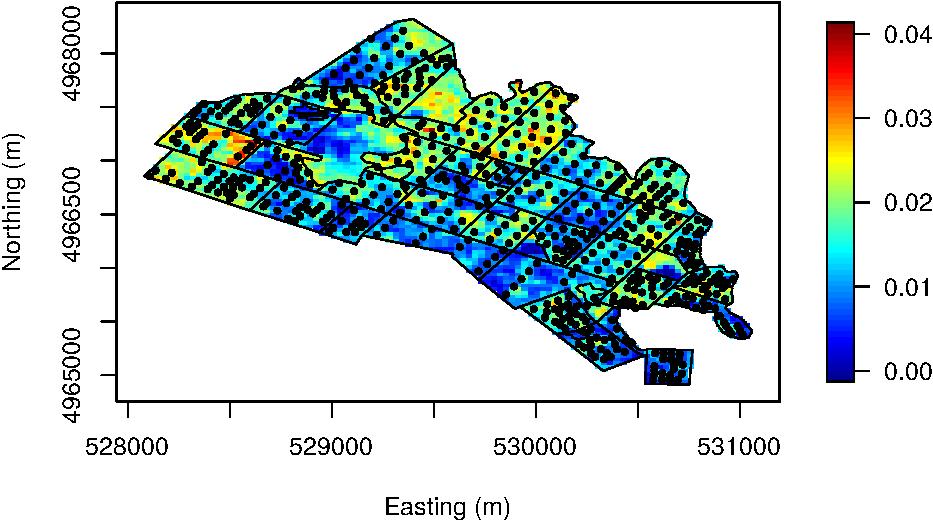
\includegraphics{bookdown_files/figure-latex/img1-1.pdf}
\caption{\label{fig:img1}Surface of LiDAR energy returns at 12 m above the
ground, forest inventory plot locations, and management unit boundaries
on the PEF.}
\end{figure}

\section{Zurichberg Forest inventory data set}\label{zf}

Measuring tree diameter and height is a time consuming process. This
fact makes the Zurichberg Forest inventory data set a rare and
impressive investment. These data comprise a complete enumeration of the
589 trees in the Zurichberg Forest, including species, diameter at
breast height, basal area, and volume. The stem map colored by species
is shown in Figure \ref{fig:zf}.

\begin{figure}
\centering
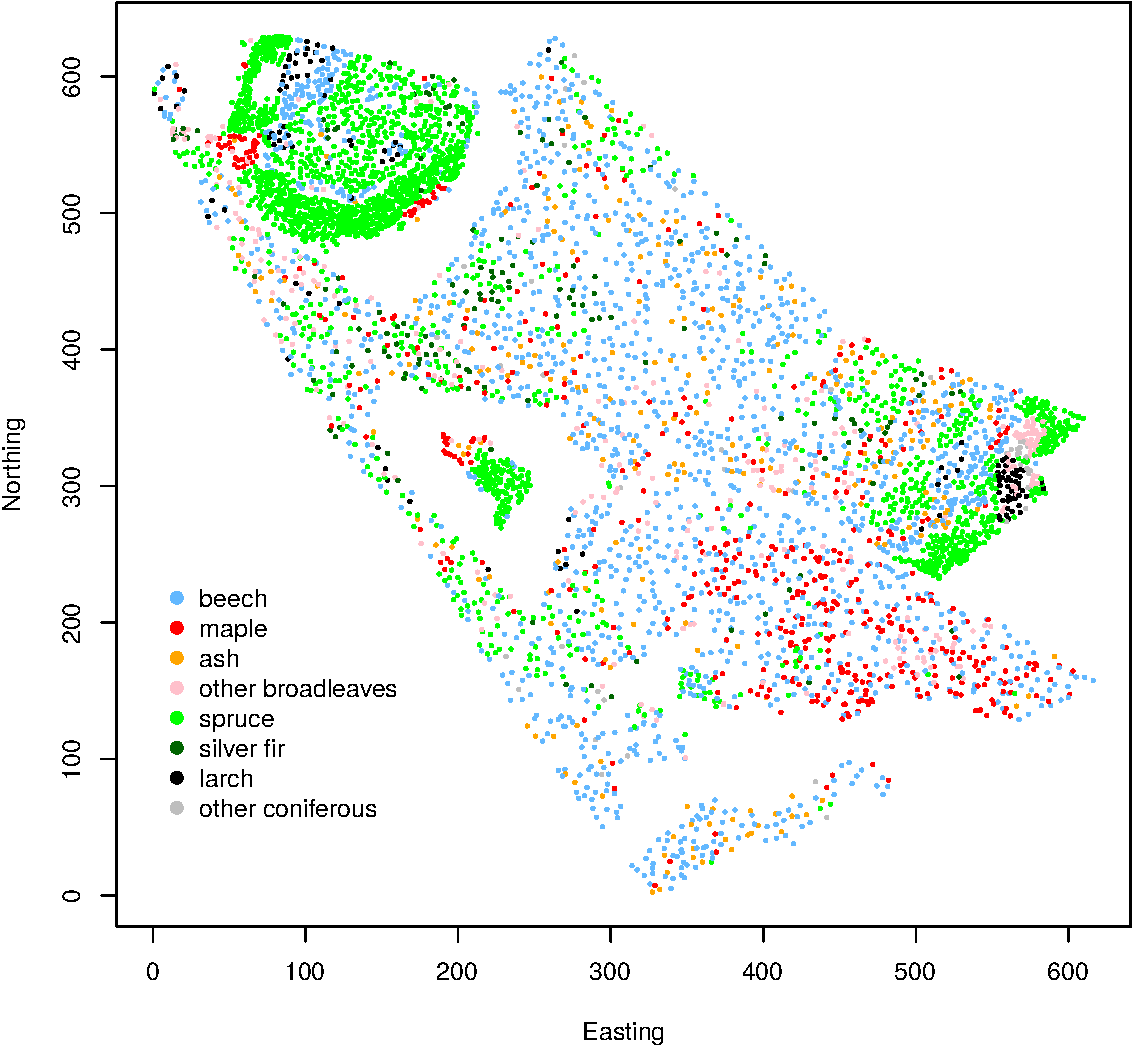
\includegraphics{bookdown_files/figure-latex/zf-1.pdf}
\caption{\label{fig:zf}Location and species of all trees in the Zurichberg
Forest.}
\end{figure}

\section{Looking Forward}\label{looking-forward}

The four examples above illustrate a variety of data sets that might be
encountered in practice, and each provides its own challenges. For the
FACE data, the challenges are more statistical in nature. Complications
could arise related to the complex study design and how that design
might affect methods of analysis and conclusions drawn from the study.
The other data sets present different challenges, such as how to:

\begin{enumerate}
\def\labelenumi{\arabic{enumi}.}
\tightlist
\item
  Develop biomass equations suitable for population inference from the
  FEF's small sample of 88 trees
\item
  Work with spatially indexed data in the case of the PEF and Zurichberg
  inventory data
\item
  Effectively and efficiently process the PEF's high-dimentional LiDAR
  signal data for use in predictive models of forest variables.
\end{enumerate}

This book and associated material introduce tools to tackle some of the
challenges in working with real data sets within the context of the R
statistical system. We will focus on important topics such as

\begin{itemize}
\tightlist
\item
  Obtaining and manipulating data
\item
  Summarizing and visualizing data
\item
  Communicating findings about data that support reproducible research
\item
  Programming and writing functions
\item
  Working with specialized data structures, e.g., spatial data and
  databases
\end{itemize}

\section{How to Learn (The Most Important Section in This
Book!)}\label{how-to-learn-the-most-important-section-in-this-book}

There are several ways to engage with the content of this book and
associated materials.

One way is not to engage at all. Leave the book closed on a shelf and do
something else with your time. That may or may not be a good life
strategy, depending on what else you do with your time, but you won't
learn much from the book!

Another way to engage is to read through the book ``passively'', reading
all that's written but not reading the book with R open on your
computer, where you could enter the R commands from the book. With this
strategy you'll probably learn more than if you leave the book closed on
a shelf, but there are better options.

A third way to engage is to read the book while you're at a computer
with R, and to enter the R commands from the book as you read about
them. You'll likely learn more this way.

A fourth strategy is even better. In addition to reading and entering
the commands given in the book, you think about what you're doing, and
ask yourself questions (which you then go on to answer). For example,
after working through some R code computing the logarithm of positive
numbers you might ask yourself, ``What would R do if I asked it to
calculate the logarithm of a negative number? What would R do if I asked
it to calculate the logarithm of a really large number such as one
trillion?'' You could explore these questions easily by just trying
things out in the R Console window.

If your goal is to maximize the time you have to binge-watch
\emph{Stranger Things} Season 2 on Netflix, the first strategy may be
optimal. But if your goal is to learn a lot about computational tools
for data science, the fourth strategy is probably going to be best.

\chapter{Introduction to R and
RStudio}\label{introduction-to-r-and-rstudio}

Various statistical and programming software environments are used in
data science, including R, Python, SAS, C++, SPSS, and many others. Each
has strengths and weaknesses, and often two or more are used in a single
project. This book focuses on R for several reasons:

\begin{enumerate}
\def\labelenumi{\arabic{enumi}.}
\tightlist
\item
  R is free
\item
  It is one of, if not the, most widely used software environments in
  data science
\item
  R is under constant and open development by a diverse and expert core
  group
\item
  It has an incredible variety of contributed packages
\item
  A new user can (relatively) quickly gain enough skills to obtain,
  manage, and analyze data in R
\end{enumerate}

Several enhanced interfaces for R have been developed. Generally such
interfaces are referred to as \emph{integrated development environments
(IDE)}. These interfaces are used to facilitate software development. At
minimum, an IDE typically consists of a source code editor and build
automation tools. We will use the RStudio IDE, which according to its
developers ``is a powerful productive user interface for R.\footnote{\url{http://www.rstudio.com/}}
RStudio is widely used, it is used increasingly in the R community, and
it makes learning to use R a bit simpler. Although we will use RStudio,
most of what is presented in this book can be accomplished in R (without
an added interface) with few or no changes.

\section{Obtaining and Installing R}\label{obtaining-and-installing-r}

It is simple to install R on computers running Microsoft Windows, macOS,
or Linux. For other operating systems users can compile the source code
directly.\footnote{Windows, macOS, and Linux users also can compile the
  source code directly, but for most it is a better idea to install R
  from already compiled binary distributions.} Here is a step-by-step
guide to installing R for Microsoft Windows.\footnote{New versions of R
  are released regularly, so the version number in Step 6 might be
  different from what is listed below.} macOS and Linux users would
follow similar steps.

\begin{enumerate}
\def\labelenumi{\arabic{enumi}.}
\tightlist
\item
  Go to \url{http://www.r-project.org/}
\item
  Click on the \texttt{CRAN} link on the left side of the page
\item
  Choose one of the mirrors.\footnote{The \url{http://cran.rstudio.com/}
    mirror is usually fast. Otherwise choose a mirror in Michigan.}
\item
  Click on \texttt{Download\ R\ for\ Windows}
\item
  Click on \texttt{base}
\item
  Click on \texttt{Download\ R\ 3.5.0\ for\ Windows}
\item
  Install R as you would install any other Windows program
\end{enumerate}

\section{Obtaining and Installing
RStudio}\label{obtaining-and-installing-rstudio}

You must install R prior to installing RStudio. RStudio is also simple
to install:

\begin{enumerate}
\def\labelenumi{\arabic{enumi}.}
\tightlist
\item
  Go to \url{http://www.rstudio.com}
\item
  Click on the link \texttt{RStudio} under the \texttt{Products} tab,
  then select the \texttt{Desktop} option
\item
  Click on the \texttt{Desktop} link
\item
  Choose the \texttt{DOWNLOAD\ RSTUDIO\ DESKTOP} link in the
  \texttt{Open\ Source\ Edition} column
\item
  On the ensuing page, click on the \texttt{Installer} version for your
  operating system, and once downloaded, install as you would any
  program
\end{enumerate}

\section{Using R and RStudio}\label{using-r-and-rstudio}

Start RStudio as you would any other program in your operating system.
For example, under Microsoft Windows use the Start Menu or double click
on the shortcut on the desktop (if a shortcut was created in the
installation process). A (rather small) view of RStudio is displayed in
Figure \ref{fig:rstudio}.

\begin{figure}
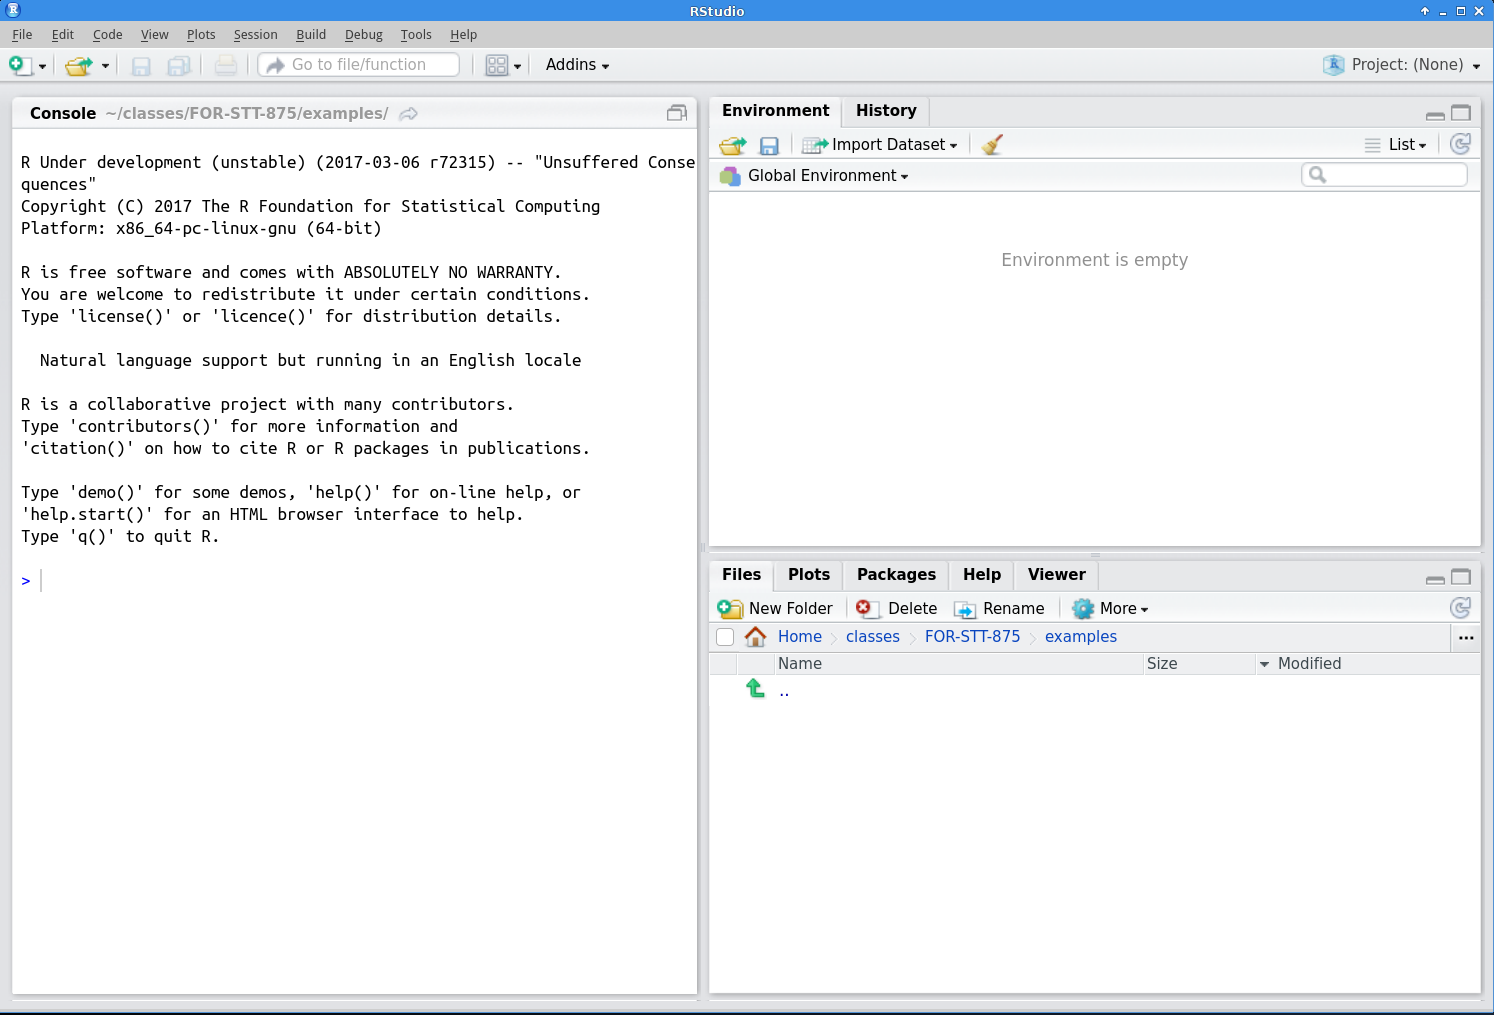
\includegraphics[width=20.75in,height=4in]{02-introToR/02-images/RStudio} \caption{The Rstudio IDE.}\label{fig:rstudio}
\end{figure}

Initially the RStudio window contains three smaller windows. For now our
main focus will be the large window on the left, the \texttt{Console}
window, in which R statements are typed. The next few sections give
simple examples of the use of R. In these sections we will focus on
small and non-complex data sets, but of course later in the book we will
work with much larger and more complex sets of data. Read these sections
at your computer with R running, and enter the R commands there to get
comfortable using the R console window and RStudio.

\subsection{R as a calculator}\label{r-as-a-calculator}

R can be used as a calculator. Note that \texttt{\#} is the comment
character in R, so R ignores everything following this character. Also,
you will see that R prints \texttt{{[}1{]}} before the results of each
command. Soon we will explain its relevance, but ignore this for now.
The command prompt in R is the greater than sign
\texttt{\textgreater{}}.

\begin{Shaded}
\begin{Highlighting}[]
\OperatorTok{>}\StringTok{ }\DecValTok{34} \OperatorTok{+}\StringTok{ }\DecValTok{20} \OperatorTok{*}\StringTok{ }\KeywordTok{sqrt}\NormalTok{(}\DecValTok{100}\NormalTok{)  ## +,-,*,/ have the expected meanings}
\end{Highlighting}
\end{Shaded}

\begin{verbatim}
[1] 234
\end{verbatim}

\begin{Shaded}
\begin{Highlighting}[]
\OperatorTok{>}\StringTok{ }\KeywordTok{exp}\NormalTok{(}\DecValTok{2}\NormalTok{)  ##The exponential function}
\end{Highlighting}
\end{Shaded}

\begin{verbatim}
[1] 7.389
\end{verbatim}

\begin{Shaded}
\begin{Highlighting}[]
\OperatorTok{>}\StringTok{ }\KeywordTok{log10}\NormalTok{(}\DecValTok{100}\NormalTok{)  ##Base 10 logarithm}
\end{Highlighting}
\end{Shaded}

\begin{verbatim}
[1] 2
\end{verbatim}

\begin{Shaded}
\begin{Highlighting}[]
\OperatorTok{>}\StringTok{ }\KeywordTok{log}\NormalTok{(}\DecValTok{100}\NormalTok{)  ##Base e logarithm}
\end{Highlighting}
\end{Shaded}

\begin{verbatim}
[1] 4.605
\end{verbatim}

\begin{Shaded}
\begin{Highlighting}[]
\OperatorTok{>}\StringTok{ }\DecValTok{10}\OperatorTok{^}\KeywordTok{log10}\NormalTok{(}\DecValTok{55}\NormalTok{)}
\end{Highlighting}
\end{Shaded}

\begin{verbatim}
[1] 55
\end{verbatim}

Most functions in R can be applied to vector arguments rather than
operating on a single argument at a time. A \emph{vector} is a data
structure that contains elements of the same data type (i.e.~integers).

\begin{Shaded}
\begin{Highlighting}[]
\OperatorTok{>}\StringTok{ }\DecValTok{1}\OperatorTok{:}\DecValTok{25}\NormalTok{  ##The integers from 1 to 25}
\end{Highlighting}
\end{Shaded}

\begin{verbatim}
 [1]  1  2  3  4  5  6  7  8  9 10 11 12 13 14 15 16 17
[18] 18 19 20 21 22 23 24 25
\end{verbatim}

\begin{Shaded}
\begin{Highlighting}[]
\OperatorTok{>}\StringTok{ }\KeywordTok{log}\NormalTok{(}\DecValTok{1}\OperatorTok{:}\DecValTok{25}\NormalTok{)  ##The base e logarithm of these integers}
\end{Highlighting}
\end{Shaded}

\begin{verbatim}
 [1] 0.0000 0.6931 1.0986 1.3863 1.6094 1.7918 1.9459
 [8] 2.0794 2.1972 2.3026 2.3979 2.4849 2.5649 2.6391
[15] 2.7081 2.7726 2.8332 2.8904 2.9444 2.9957 3.0445
[22] 3.0910 3.1355 3.1781 3.2189
\end{verbatim}

\begin{Shaded}
\begin{Highlighting}[]
\OperatorTok{>}\StringTok{ }\DecValTok{1}\OperatorTok{:}\DecValTok{25} \OperatorTok{*}\StringTok{ }\DecValTok{1}\OperatorTok{:}\DecValTok{25}\NormalTok{  ##What will this produce?}
\end{Highlighting}
\end{Shaded}

\begin{verbatim}
 [1]   1   4   9  16  25  36  49  64  81 100 121 144
[13] 169 196 225 256 289 324 361 400 441 484 529 576
[25] 625
\end{verbatim}

\begin{Shaded}
\begin{Highlighting}[]
\OperatorTok{>}\StringTok{ }\DecValTok{1}\OperatorTok{:}\DecValTok{25} \OperatorTok{*}\StringTok{ }\DecValTok{1}\OperatorTok{:}\DecValTok{5}\NormalTok{  ##What about this?}
\end{Highlighting}
\end{Shaded}

\begin{verbatim}
 [1]   1   4   9  16  25   6  14  24  36  50  11  24
[13]  39  56  75  16  34  54  76 100  21  44  69  96
[25] 125
\end{verbatim}

\begin{Shaded}
\begin{Highlighting}[]
\OperatorTok{>}\StringTok{ }\KeywordTok{seq}\NormalTok{(}\DataTypeTok{from =} \DecValTok{0}\NormalTok{, }\DataTypeTok{to =} \DecValTok{1}\NormalTok{, }\DataTypeTok{by =} \FloatTok{0.1}\NormalTok{)  ##A sequence of numbers from 0 to 1}
\end{Highlighting}
\end{Shaded}

\begin{verbatim}
 [1] 0.0 0.1 0.2 0.3 0.4 0.5 0.6 0.7 0.8 0.9 1.0
\end{verbatim}

\begin{Shaded}
\begin{Highlighting}[]
\OperatorTok{>}\StringTok{ }\KeywordTok{exp}\NormalTok{(}\KeywordTok{seq}\NormalTok{(}\DataTypeTok{from =} \DecValTok{0}\NormalTok{, }\DataTypeTok{to =} \DecValTok{1}\NormalTok{, }\DataTypeTok{by =} \FloatTok{0.1}\NormalTok{))  ##What will this produce?}
\end{Highlighting}
\end{Shaded}

\begin{verbatim}
 [1] 1.000 1.105 1.221 1.350 1.492 1.649 1.822 2.014
 [9] 2.226 2.460 2.718
\end{verbatim}

Now the mysterious square bracketed numbers appearing next to the output
make sense. R puts the position of the beginning value on a line in
square brackets before the line of output. For example if the output has
40 values, and 15 values appear on each line, then the first line will
have \texttt{{[}1{]}} at the left, the second line will have
\texttt{{[}16{]}} to the left, and the third line will have
\texttt{{[}31{]}} to the left.

\subsection{Basic descriptive statistics and graphics in
R}\label{sec:dec}

Of course it is easy to compute basic descriptive statistics and to
produce standard graphical representations of data. For illustration
consider the first 14 observations of tree height and DBH (diameter at
breast height) from the FEF data set. We will begin by entering these
data ``by hand'' using the \texttt{c()} function, which concatenates its
arguments into a vector. For larger data sets we will clearly want an
alternative way to enter data.

A style note: R has two widely used methods of assignment: the left
arrow, which consists of a less than sign followed immediately by a
dash: \texttt{\textless{}-} and the equals sign: \texttt{=}. Much ink
has been used debating the relative merits of the two methods, and their
subtle differences. Many leading R style guides (e.g., the Google style
guide at \url{https://google.github.io/styleguide/Rguide.xml} and the
Bioconductor style guide at
\url{http://www.bioconductor.org/developers/how-to/coding-style/})
recommend the left arrow \texttt{\textless{}-} as an assignment
operator, and we will use this throughout the book.

Also you will see that if a command has not been completed but the ENTER
key is pressed, the command prompt changes to a \texttt{+} sign.

\begin{Shaded}
\begin{Highlighting}[]
\OperatorTok{>}\StringTok{ }\NormalTok{dbh <-}\StringTok{ }\KeywordTok{c}\NormalTok{(}\DecValTok{6}\NormalTok{, }\FloatTok{6.9}\NormalTok{, }\FloatTok{6.4}\NormalTok{, }\FloatTok{6.5}\NormalTok{, }\FloatTok{7.2}\NormalTok{, }\FloatTok{3.1}\NormalTok{, }\DecValTok{2}\NormalTok{, }\FloatTok{4.1}\NormalTok{, }\FloatTok{2.4}\NormalTok{, }\FloatTok{2.7}\NormalTok{, }\FloatTok{3.7}\NormalTok{, }
\OperatorTok{+}\StringTok{   }\FloatTok{6.3}\NormalTok{, }\FloatTok{5.2}\NormalTok{, }\FloatTok{5.1}\NormalTok{, }\FloatTok{6.4}\NormalTok{)}
\OperatorTok{>}\StringTok{ }\NormalTok{ht <-}\StringTok{ }\KeywordTok{c}\NormalTok{(}\DecValTok{48}\NormalTok{, }\DecValTok{48}\NormalTok{, }\DecValTok{48}\NormalTok{, }\DecValTok{49}\NormalTok{, }\DecValTok{51}\NormalTok{, }\DecValTok{40}\NormalTok{, }\FloatTok{30.5}\NormalTok{, }\DecValTok{50}\NormalTok{, }\DecValTok{28}\NormalTok{, }\FloatTok{40.4}\NormalTok{, }\FloatTok{42.6}\NormalTok{, }
\OperatorTok{+}\StringTok{   }\DecValTok{53}\NormalTok{, }\DecValTok{55}\NormalTok{, }\DecValTok{50}\NormalTok{, }\DecValTok{50}\NormalTok{)}
\OperatorTok{>}\StringTok{ }\NormalTok{dbh}
\end{Highlighting}
\end{Shaded}

\begin{verbatim}
 [1] 6.0 6.9 6.4 6.5 7.2 3.1 2.0 4.1 2.4 2.7 3.7 6.3
[13] 5.2 5.1 6.4
\end{verbatim}

\begin{Shaded}
\begin{Highlighting}[]
\OperatorTok{>}\StringTok{ }\NormalTok{ht}
\end{Highlighting}
\end{Shaded}

\begin{verbatim}
 [1] 48.0 48.0 48.0 49.0 51.0 40.0 30.5 50.0 28.0 40.4
[11] 42.6 53.0 55.0 50.0 50.0
\end{verbatim}

Next we compute some descriptive statistics for the two numeric
variables

\begin{Shaded}
\begin{Highlighting}[]
\OperatorTok{>}\StringTok{ }\KeywordTok{mean}\NormalTok{(dbh)}
\end{Highlighting}
\end{Shaded}

\begin{verbatim}
[1] 4.933
\end{verbatim}

\begin{Shaded}
\begin{Highlighting}[]
\OperatorTok{>}\StringTok{ }\KeywordTok{sd}\NormalTok{(dbh)}
\end{Highlighting}
\end{Shaded}

\begin{verbatim}
[1] 1.782
\end{verbatim}

\begin{Shaded}
\begin{Highlighting}[]
\OperatorTok{>}\StringTok{ }\KeywordTok{summary}\NormalTok{(dbh)}
\end{Highlighting}
\end{Shaded}

\begin{verbatim}
   Min. 1st Qu.  Median    Mean 3rd Qu.    Max. 
   2.00    3.40    5.20    4.93    6.40    7.20 
\end{verbatim}

\begin{Shaded}
\begin{Highlighting}[]
\OperatorTok{>}\StringTok{ }\KeywordTok{mean}\NormalTok{(ht)}
\end{Highlighting}
\end{Shaded}

\begin{verbatim}
[1] 45.57
\end{verbatim}

\begin{Shaded}
\begin{Highlighting}[]
\OperatorTok{>}\StringTok{ }\KeywordTok{sd}\NormalTok{(ht)}
\end{Highlighting}
\end{Shaded}

\begin{verbatim}
[1] 7.857
\end{verbatim}

\begin{Shaded}
\begin{Highlighting}[]
\OperatorTok{>}\StringTok{ }\KeywordTok{summary}\NormalTok{(ht)}
\end{Highlighting}
\end{Shaded}

\begin{verbatim}
   Min. 1st Qu.  Median    Mean 3rd Qu.    Max. 
   28.0    41.5    48.0    45.6    50.0    55.0 
\end{verbatim}

Next, a scatter plot of \texttt{dbh} versus \texttt{ht}:

\begin{Shaded}
\begin{Highlighting}[]
\OperatorTok{>}\StringTok{ }\KeywordTok{plot}\NormalTok{(dbh, ht)}
\end{Highlighting}
\end{Shaded}

\begin{center}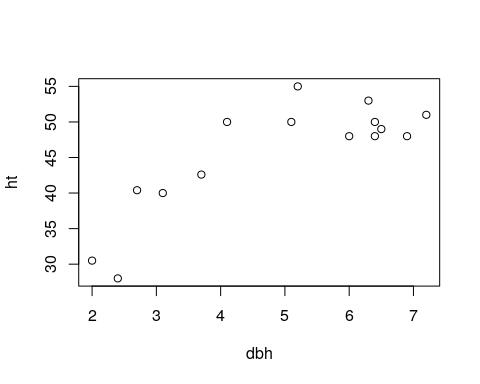
\includegraphics{bookdown_files/figure-latex/unnamed-chunk-4-1} \end{center}

Unsurprisingly as DBH increases, height tends to increase. We'll
investigate this further using simple linear regression in the next
section.

\subsection{Simple linear regression in
R}\label{simple-linear-regression-in-r}

The \texttt{lm()} function is used to fit linear models in R, including
simple linear regression models. Here it is applied to the DBH height
data.

\begin{Shaded}
\begin{Highlighting}[]
\OperatorTok{>}\StringTok{ }\NormalTok{ht.lm <-}\StringTok{ }\KeywordTok{lm}\NormalTok{(ht }\OperatorTok{~}\StringTok{ }\NormalTok{dbh)  ##Fit the model and save it in ht.lm}
\OperatorTok{>}\StringTok{ }\KeywordTok{summary}\NormalTok{(ht.lm)  ##Basic summary of the model}
\end{Highlighting}
\end{Shaded}

\begin{verbatim}

Call:
lm(formula = ht ~ dbh)

Residuals:
   Min     1Q Median     3Q    Max 
-8.507 -2.742 -0.812  2.683  8.480 

Coefficients:
            Estimate Std. Error t value Pr(>|t|)    
(Intercept)   27.925      3.739    7.47  4.7e-06 ***
dbh            3.576      0.716    5.00  0.00024 ***
---
Signif. codes:  
0 '***' 0.001 '**' 0.01 '*' 0.05 '.' 0.1 ' ' 1

Residual standard error: 4.77 on 13 degrees of freedom
Multiple R-squared:  0.658, Adjusted R-squared:  0.631 
F-statistic:   25 on 1 and 13 DF,  p-value: 0.000244
\end{verbatim}

\begin{Shaded}
\begin{Highlighting}[]
\OperatorTok{>}\StringTok{ }\KeywordTok{plot}\NormalTok{(dbh, ht)  ##Scatter plot of the data}
\OperatorTok{>}\StringTok{ }\KeywordTok{abline}\NormalTok{(ht.lm)  ##Add the fitted regression line to the plot}
\end{Highlighting}
\end{Shaded}

\begin{center}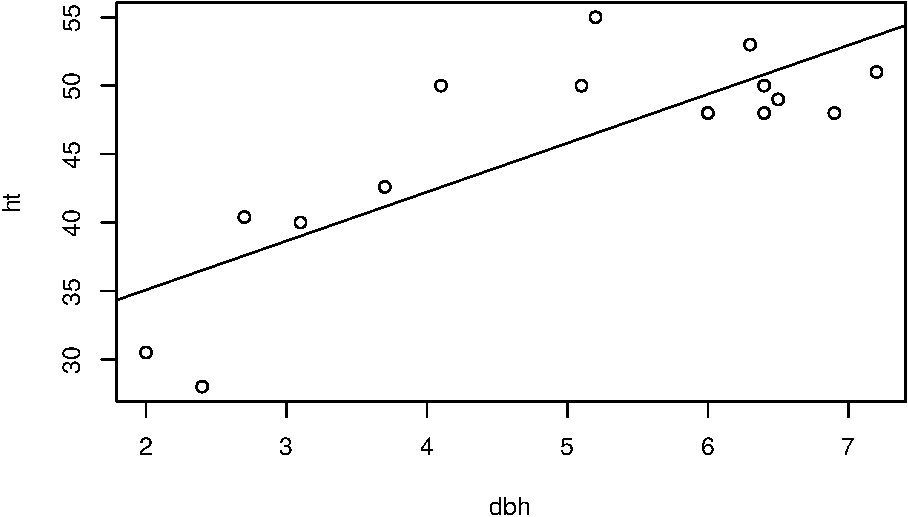
\includegraphics{bookdown_files/figure-latex/unnamed-chunk-5-1} \end{center}

We will work extensively with such models later in the text. We will
also talk about why it might not be a good idea to assume a linear
relationship between DBH and height---can you guess why this is by
looking at the data scatter and model fitted line in the plot above?

\section{How to Learn}\label{how-to-learn}

There are several ways to engage with the content of this book and
associated learning materials.

A comprehensive, but slightly overwhelming, cheatsheet for RStudio is
available here
\url{https://www.rstudio.com/wp-content/uploads/2016/01/rstudio-IDE-cheatsheet.pdf}.
As we progress in learning R and RStudio, this cheatsheet will become
more useful. For now you might use the cheatsheet to locate the various
windows and functions identified in the coming chapters.

\section{Getting help}\label{getting-help}

There are several free (and several not free) ways to get R help when
needed.

Several help-related functions are built into R. If there's a particular
R function of interest, such as \texttt{log}, \texttt{help(log)} or
\texttt{?log} will bring up a help page for that function. In RStudio
the help page is displayed, by default, in the \texttt{Help} tab in the
lower right window.\footnote{There are ways to change this default
  behavior.} The function \texttt{help.start} opens a window which
allows browsing of the online documentation included with R. To use
this, type \texttt{help.start()} in the console window.\footnote{You may
  wonder about the parentheses after \texttt{help.start}. A user can
  specify arguments to any R function inside parentheses. For example
  \texttt{log(10)} asks R to return the logarithm of the argument 10.
  Even if no arguments are needed, R requires empty parentheses at the
  end of any function name. In fact if you just type the function name
  without parentheses, R returns the definition of the function. For
  simple functions this can be illuminating.} The \texttt{help.start}
function also provides several manuals online and can be a useful
interface in addition to the built in help.

Search engines provide another, sometimes more user-friendly, way to
receive answers for R questions. A Google search often quickly finds
something written by another user who had the same (or a similar)
question, or an online tutorial that touches on the question. More
specialized is \url{https://rseek.org/}, which is a search engine
focused specifically on R. Both Google and \url{https://rseek.org} are
valuable tools, often providing more user-friendly information then R's
own help system.

In addition, R users have written many types of contributed
documentation. Some of this documentation is available at
\url{http://cran.r-project.org/other-docs.html}. Of course there are
also numerous books covering general and specialized R topics available
for purchase.

\section{Workspace, working directory, and keeping
organized}\label{workspace-working-directory-and-keeping-organized}

The \emph{workspace} is your R session working environment and includes
any objects you create. Recall these objects are listed in the
\texttt{Global\ Environment} window. The command \texttt{ls()}, which
stands for list, will also list all the objects in your workspace (note,
this is the same list that is given in the \texttt{Global\ Environment}
window). When you close RStudio, a dialog box will ask you if you want
to save an image of the current workspace. If you choose to save your
workspace, RStudio saves your session objects and information in a
\texttt{.RData} file (the period makes it a hidden file) in your
\emph{working directory}. Next time you start R or RStudio it checks if
there is a \texttt{.RData} in the working directory, loads it if it
exists, and your session continues where you left off. Otherwise R
starts with an empty workspace. This leads to the next question---what
is a working directory?

Each R session is associated with a working directory. This is just a
directory from which R reads and writes files, e.g., the \texttt{.RData}
file, data files you want to analyze, or files you want to save. On Mac
when you start RStudio it sets the working directory to your home
directory (for me that's \texttt{/Users/andy}). If you're on a different
operating system, you can check where the default working directory is
by typing \texttt{getwd()} in the console. You can change the default
working directory under RStudio's \texttt{Global\ Option} dialog found
under the \texttt{Tools} dropdown menu. There are multiple ways to
change the working directory once an R session is started in RStudio.
One method is to click on the \texttt{Files} tab in the lower right
window and then click the \texttt{More} button. Alternatively, you can
set the session's working directory using the \texttt{setwd()} in the
console. For example, on Windows
\texttt{setwd("C:/Users/andy/for472/exercise1")} will set the working
directory to \texttt{C:/Users/andy/for472/exercise1}, assuming that file
path and directory exist (Note: Windows file path uses a backslash,
\texttt{\textbackslash{}}, but in R the backslash is an escape
character, hence specifying file paths in R on Windows uses the forward
slash, i.e., \texttt{/}). Similarly on Mac you can use
\texttt{setwd("/Users/andy/for472/exercise1")}. Perhaps the most simple
method is to click on the \texttt{Session} tab at the top of your screen
and click on the \texttt{Set\ Working\ Directory} option. Later on when
we start reading and writing data from our R session, it will be very
important that you are able to identify your current working directory
and change it if needed. We will revisit this in subsequent chapters.

As with all work, keeping organized is the key to efficiency. It is good
practice to have a dedicated directory for each R project or exercise.

\section{Quality of R code}\label{quality-of-r-code}

\begin{figure}
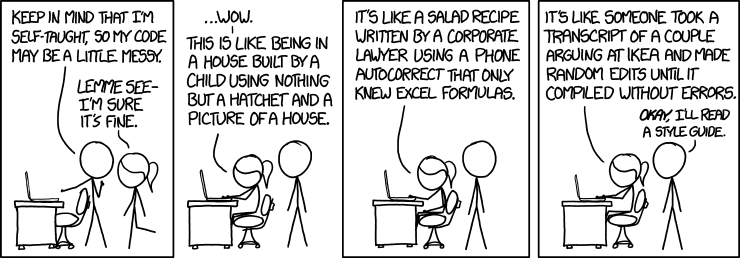
\includegraphics[width=4in,height=4in]{02-introToR/02-images/code_quality} \caption{xkcd: Code Quality}\label{fig:comic}
\end{figure}

Writing well-organized and well-labeled code allows your code to be more
easily read and understood by another person. (See xkcd's take on code
quality in Figure \ref{fig:comic}.) More importantly, though, your
well-written code is more accessible to you hours, days, or even months
later. We are hoping that you can use the code you write in this class
in future projects and research.

Google provides style guides for many programming languages. You can
find the R style guide
\href{https://google.github.io/styleguide/Rguide.xml}{here}. Below are a
few of the key points from the guide that we will use right away.

\subsection{Naming Files}\label{naming-files}

File names should be meaningful and end in \texttt{.R}. If we write a
script that analyzes a certain species distribution:

\begin{itemize}
\tightlist
\item
  GOOD: \(\color{green}{\verb+african_rhino_distribution.R+}\)
\item
  GOOD: \(\color{green}{\verb+africanRhinoDistribution.R+}\)
\item
  BAD: \(\color{red}{\verb+speciesDist.R+}\) (too ambiguous)
\item
  BAD: \(\color{red}{\verb+species.dist.R+}\) (too ambiguous and two
  periods can confuse operating systems' file type auto-detect)
\item
  BAD: \(\color{red}{\verb+speciesdist.R+}\) (too ambiguous and
  confusing)
\end{itemize}

\subsection{Naming Variables}\label{naming-variables}

\begin{itemize}
\tightlist
\item
  GOOD: \(\color{green}{\verb+rhino.count+}\)
\item
  GOOD: \(\color{green}{\verb+rhinoCount+}\)
\item
  GOOD: \(\color{green}{\verb+rhino_count+}\) (We don't mind the
  underscore and use it quite often, although Google's style guide says
  it's a no-no for some reason)
\item
  BAD: \(\color{red}{\verb+rhinocount+}\) (confusing)
\end{itemize}

\subsection{Syntax}\label{syntax}

\begin{itemize}
\tightlist
\item
  Keep code lines under 80 characters long.
\item
  Indent your code with two spaces. (RStudio does this by default when
  you press the TAB key.)
\end{itemize}

\chapter{Scripts, R Markdown, and Reproducible
Research}\label{scripts-r-markdown-and-reproducible-research}

Doing work in data science, whether for homework, a project for a
business, or a research project, typically involves several iterations.
For example, creating an effective graphical representation of data can
involve trying out several different graphical representations, and then
tens if not hundreds of iterations when fine-tuning the chosen
representation. And each of these representations may require several R
commands to create. Although this all could be accomplished by typing
and re-typing commands at the R Console, it is easier and more effective
to write the commands in a \emph{script file} that can then be submitted
to the R console either a line at a time or all together.\footnote{Unsurprisingly
  it is also possible to submit several selected lines of code at once.}

In addition to making the workflow more efficient, R scripts provide
another large benefit. Often we work on one part of a homework
assignment or project for a few hours, then move on to something else,
and then return to the original part a few days, months, or sometimes
even years later. In such cases we may have forgotten how we created a
graphical display that we were so proud of, and will again need to spend
a few hours to recreate it. If we save a script file, we have the
ingredients immediately available when we return to a portion of a
project.\footnote{In principle the R history mechanism provides a
  similar record. But with history we have to search through a lot of
  other code to find what we're looking for, and scripts are a much
  cleaner mechanism to record our work.}

Next consider a larger scientific endeavor. Ideally a scientific study
will be reproducible, meaning that an independent group of researchers
(or the original researchers) will able to duplicate the study. Thinking
about data science, this means that all the steps taken when working
with the data from a study should be reproducible, from selection of
variables to formal data analysis. In principle this can be facilitated
by explaining, in words, each step of the work with data. In practice,
on the other hand, it is typically difficult or impossible to reproduce
a full data analysis based on a written explanation. It is much more
effective to include the actual computer code that accomplished the data
work in the report, whether the report is a homework assignment or a
research paper. Tools in R such as \emph{R Markdown} facilitate this
process.

\section{Scripts in R}\label{scripts-in-r}

As noted above, scripts help to make working with data more efficient
and provide a record of how data were managed and analyzed. Here we
describe an example using the FEF data.\footnote{The example uses
  features of R that we have not yet discussed, so don't worry about the
  details but rather about how it motivates the use of a script file.}
First we read the FEF data into R using the code below.

\begin{Shaded}
\begin{Highlighting}[]
\OperatorTok{>}\StringTok{ }\NormalTok{face.dat <-}\StringTok{ }\KeywordTok{read.csv}\NormalTok{(}
\OperatorTok{+}\StringTok{     }\DataTypeTok{file=}\StringTok{"http://blue.for.msu.edu/FOR472/data/FACE_aspen_core_growth.csv"}
\OperatorTok{+}\StringTok{ }\NormalTok{)}
\end{Highlighting}
\end{Shaded}

Next we print the names of the variables in the data set. Don't be
concerned about the specific details. Later we will learn much more
about reading in data and working with data sets in R.

\begin{Shaded}
\begin{Highlighting}[]
\OperatorTok{>}\StringTok{ }\KeywordTok{names}\NormalTok{(face.dat)}
\end{Highlighting}
\end{Shaded}

\begin{verbatim}
 [1] "Rep"                 "Treat"              
 [3] "Clone"               "E.Clone"            
 [5] "Row"                 "Col"                
 [7] "ID.."                "X1997Initial_Height"
 [9] "X1997Initial_Diam"   "X1997Final_Height"  
[11] "X1997Final_Diam"     "X1998_Height"       
[13] "X1998_Diam"          "X1999_Height"       
[15] "X1999_Diam"          "X2000_Height"       
[17] "X2000_Diam"          "X2001_Height"       
[19] "X2001_AvgDiam"       "X2001_Diam.3cm"     
[21] "X2001_Diam.10cm"     "X2002_Height"       
[23] "X2002_Diam.10cm"     "X2003_Height"       
[25] "X2003_Diam.10cm"     "X2003_DBH"          
[27] "X2004_Height"        "X2004_Diam.10cm"    
[29] "X2004_DBH"           "X2005_Height"       
[31] "X2005_Diam.10cm"     "X2005_DBH"          
[33] "X2006_Height"        "X2006_DBH"          
[35] "X2007_Height"        "X2007_DBH"          
[37] "X2008_Height"        "X2008_DBH"          
[39] "Notes"               "Comment1"           
[41] "Comment2"            "Comment3"           
[43] "Comment4"            "Comment5"           
[45] "Comment6"           
\end{verbatim}

Let's create a scatter plot of 2008 DBH versus height. To do this we'll
first create variables for DBH and height taken in the year 2008 and
print out the first ten values of each variable.\footnote{Neither of
  these steps are necessary, but are convenient for illustration.}

\begin{Shaded}
\begin{Highlighting}[]
\OperatorTok{>}\StringTok{ }\NormalTok{dbh <-}\StringTok{ }\NormalTok{face.dat}\OperatorTok{$}\NormalTok{X2008_DBH}
\OperatorTok{>}\StringTok{ }\NormalTok{ht <-}\StringTok{ }\NormalTok{face.dat}\OperatorTok{$}\NormalTok{X2008_Height}
\OperatorTok{>}\StringTok{ }\NormalTok{dbh[}\DecValTok{1}\OperatorTok{:}\DecValTok{10}\NormalTok{]}
\end{Highlighting}
\end{Shaded}

\begin{verbatim}
 [1]   NA 9.55 2.00 9.00 3.11 6.35 4.60   NA   NA 1.42
\end{verbatim}

\begin{Shaded}
\begin{Highlighting}[]
\OperatorTok{>}\StringTok{ }\NormalTok{ht[}\DecValTok{1}\OperatorTok{:}\DecValTok{10}\NormalTok{]}
\end{Highlighting}
\end{Shaded}

\begin{verbatim}
 [1]   NA 1225  334 1079  370  859  818   NA   NA  268
\end{verbatim}

The \texttt{NA} is how missing data are represented in R. Their presence
here suggests several trees in this data set are dead or not measured
for some reason in 2008. Of course at some point it would be good to
investigate which trees have missing data and why. The \texttt{plot()}
function in R will omit missing values, and for now we will just plot
the non-missing data. A scatter plot of the data is drawn next.

\begin{Shaded}
\begin{Highlighting}[]
\OperatorTok{>}\StringTok{ }\KeywordTok{plot}\NormalTok{(dbh, ht)}
\end{Highlighting}
\end{Shaded}

\begin{center}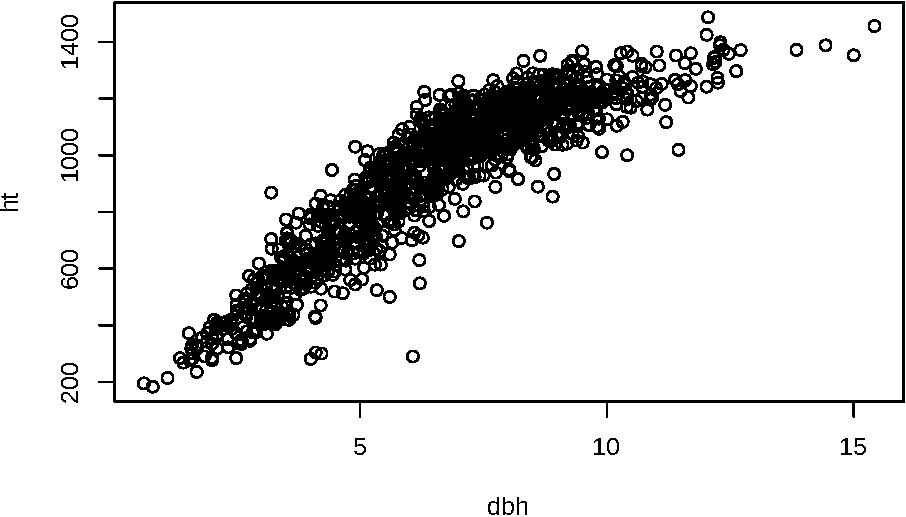
\includegraphics{bookdown_files/figure-latex/unnamed-chunk-9-1} \end{center}

Not surprisingly, the scatter plot shows that DBH and height are
positively correlated and the relationship is nonlinear. Now that we
have a basic scatter plot, it is tempting to make it more informative.
We will do this by adding a feature that identifies which trees belong
to the control and elevated CO\(_2\) environment treatments. We do this
by first separating DBH and height into their respective treatment
groups.

\begin{Shaded}
\begin{Highlighting}[]
\OperatorTok{>}\StringTok{ }\NormalTok{treat <-}\StringTok{ }\NormalTok{face.dat}\OperatorTok{$}\NormalTok{Treat}
\OperatorTok{>}\StringTok{ }\NormalTok{dbh.treat.}\DecValTok{1}\NormalTok{ <-}\StringTok{ }\NormalTok{dbh[treat }\OperatorTok{==}\StringTok{ }\DecValTok{1}\NormalTok{]  ##Treatment 1 is the control}
\OperatorTok{>}\StringTok{ }\NormalTok{ht.treat.}\DecValTok{1}\NormalTok{ <-}\StringTok{ }\NormalTok{ht[treat }\OperatorTok{==}\StringTok{ }\DecValTok{1}\NormalTok{]}
\OperatorTok{>}\StringTok{ }
\ErrorTok{>}\StringTok{ }\NormalTok{dbh.treat.}\DecValTok{2}\NormalTok{ <-}\StringTok{ }\NormalTok{dbh[treat }\OperatorTok{==}\StringTok{ }\DecValTok{2}\NormalTok{]  ##Treatment 2 is the elevated CO2}
\OperatorTok{>}\StringTok{ }\NormalTok{ht.treat.}\DecValTok{2}\NormalTok{ <-}\StringTok{ }\NormalTok{ht[treat }\OperatorTok{==}\StringTok{ }\DecValTok{2}\NormalTok{]}
\end{Highlighting}
\end{Shaded}

To make a more informative scatter plot we will do two things. First
make a plot for treatment 1 data, but ensure the plot region is large
enough to include the treatment 2 data. This is done by specifying the
range of the plot axes via \texttt{xlim} and \texttt{ylim} arguments in
the \texttt{plot()} function. Here the \texttt{xlim} and \texttt{ylim}
are set to the range of \texttt{dbh} and \texttt{ht} values,
respectively, using \texttt{range()} (try and figure out what the
\texttt{na.rm} argument does in the range function). Second we add
treatment 2 data via the \texttt{points()} function. There are several
other arguments passed to the plot function, but don't worry about these
details for now.

\begin{Shaded}
\begin{Highlighting}[]
\OperatorTok{>}\StringTok{ }\KeywordTok{plot}\NormalTok{(dbh.treat.}\DecValTok{1}\NormalTok{, ht.treat.}\DecValTok{1}\NormalTok{, }\DataTypeTok{xlim =} \KeywordTok{range}\NormalTok{(dbh, }\DataTypeTok{na.rm =} \OtherTok{TRUE}\NormalTok{), }
\OperatorTok{+}\StringTok{   }\DataTypeTok{ylim =} \KeywordTok{range}\NormalTok{(ht, }\DataTypeTok{na.rm =} \OtherTok{TRUE}\NormalTok{), }\DataTypeTok{pch =} \DecValTok{19}\NormalTok{, }\DataTypeTok{col =} \StringTok{"salmon3"}\NormalTok{, }
\OperatorTok{+}\StringTok{   }\DataTypeTok{cex =} \FloatTok{0.5}\NormalTok{, }\DataTypeTok{xlab =} \StringTok{"DBH (cm)"}\NormalTok{, }\DataTypeTok{ylab =} \StringTok{"Height (cm)"}\NormalTok{)}
\OperatorTok{>}\StringTok{ }\KeywordTok{points}\NormalTok{(dbh.treat.}\DecValTok{2}\NormalTok{, ht.treat.}\DecValTok{2}\NormalTok{, }\DataTypeTok{pch =} \DecValTok{19}\NormalTok{, }\DataTypeTok{col =} \StringTok{"blue"}\NormalTok{, }
\OperatorTok{+}\StringTok{   }\DataTypeTok{cex =} \FloatTok{0.5}\NormalTok{)}
\end{Highlighting}
\end{Shaded}

\begin{center}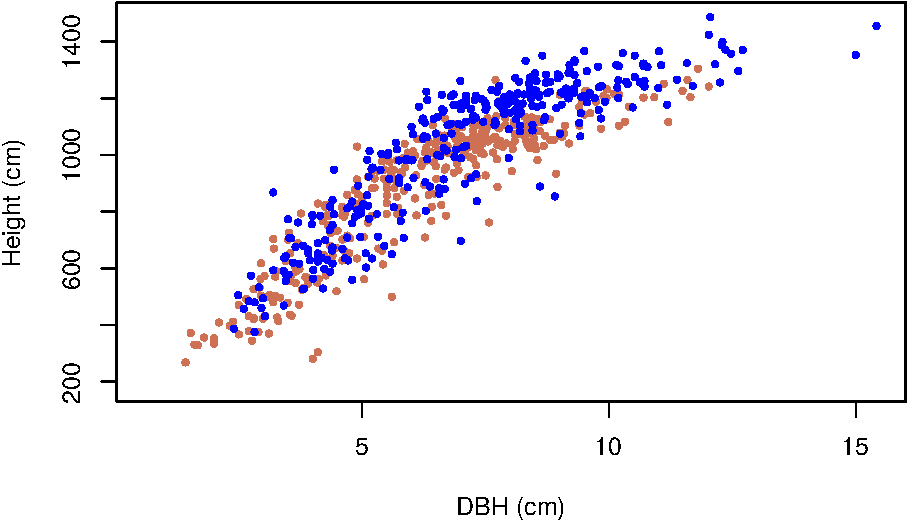
\includegraphics{bookdown_files/figure-latex/unnamed-chunk-11-1} \end{center}

Of course we should have a plot legend to tell the viewer which colors
are associated with the treatments, as well as many other aesthetic
refinements. For now, however, we will resist such
temptations.\footnote{As an aside, by only looking at the plotted data
  and thinking about basic plant physiology, can you guess which color
  is associated with the elevated CO\(_2\) treatment?}

Some of the process leading to the completed plot is shown above. We
read in the data, created an intermediate plot by adding treatment
identifiers, creating variables representing the 2008 measurements of
DBH and height, and so on. However, a lot of the process isn't shown.
For example, I made several mistakes in the process of getting the code
and plot the way I wanted it---forgot the \texttt{na.rm=TRUE} initially
then fiddled around with the treatment colors a bit.

Now imagine trying to recreate the plot a few days later. Possibly
someone saw the plot and commented that it would be interesting to see
similar plots for each year in the study period. If we did all the work,
including all the false starts and refinements, at the console it would
be hard to sort things out. This would take much longer than necessary
to create the new plots. This would be especially true if a few months
had passed, rather than just a few days.

Creating the new scatter plots would be much easier with a script file,
especially if it had a few well-chosen comments. Fortunately it is quite
easy to create and work with script files in RStudio.\footnote{It is
  also easy in R without RStudio. Just use
  \texttt{File\ \textgreater{}\ New\ script} to create a script file,
  and save it before exiting R.} Just choose
\texttt{File\ \textgreater{}\ New\ File\ \textgreater{}\ New\ script}
and a script window will open up in the upper left of the full RStudio
window.

An example of a script window (with some R code already typed in) is
shown in Figure \ref{fig:script}. From the script window the user can,
among other things, save the script (either using the \texttt{File} menu
or the icon near the top left of the window) and can run one or more
lines of code from the window (using the \texttt{run} icon in the
window, or by copying and pasting into the console window). In addition,
there is a \texttt{Source\ on\ Save} checkbox. If this is checked, the R
code in the script window is automatically read into R and executed when
the script file is saved.

\begin{figure}

{\centering 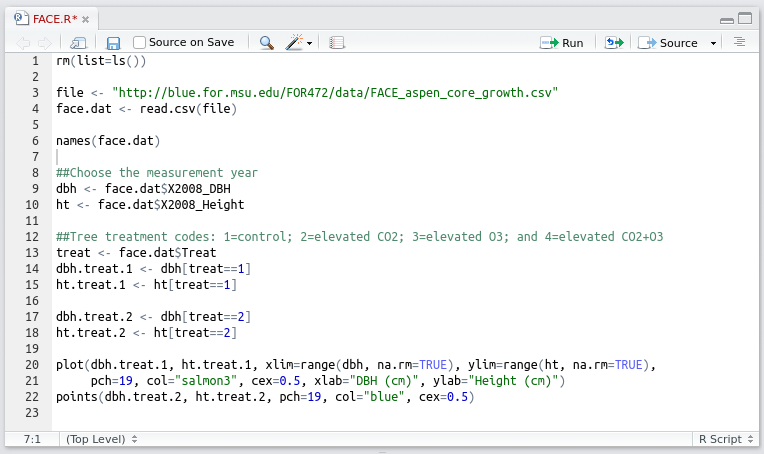
\includegraphics[width=1\linewidth]{03-scripts/03-images/FACE-script-screenshot} 

}

\caption{A script window in RStudio}\label{fig:script}
\end{figure}

\section{R Markdown}\label{r-markdown}

People typically work on data with a larger purpose in mind. Possibly
the purpose is to understand a biological system more clearly. Possibly
the purpose is to refine a system that recommends movies to users in an
online streaming movie service. Possibly the purpose is to complete a
homework assignment and demonstrate to the instructor an understanding
of an aspect of data analysis. Whatever the purpose, a key aspect is
communicating with the desired audience.

One possibility, which is somewhat effective, is to write a document
using software such as Microsoft Word \footnote{Or possibly LaTeX if the
  document is more technical} and to include R output such as
computations and graphics by cutting and pasting into the main document.
One drawback to this approach is similar to what makes script files so
useful: If the document must be revised it may be hard to unearth the R
code that created graphics or analyses, to revise these.\footnote{Organizing
  the R code using script files and keeping all the work organized in a
  well-thought-out directory structure can help here, but this requires
  a level of forethought and organization that most people do not
  possess \(\ldots\) including myself.} A more subtle but possibly more
important drawback is that the reader of the document will not know
precisely how analyses were done, or how graphics were created. Over
time even the author(s) of the paper will forget the details. A verbal
description in a ``methods'' section of a paper can help here, but
typically these do not provide all the details of the analysis, but
rather might state something like, ``All analyses were carried out using
R version 3.3.1.''

RStudio's website provides an excellent overview of R Markdown
capabilities for reproducible research. At minimum, follow the
\texttt{Get\ Started} link at \url{http://rmarkdown.rstudio.com/} and
watch the introduction video.

Among other things, R Markdown provides a way to include R code that
read in data, create graphics, or perform analyses, all in a single
document that is processed to create a research paper, homework
assignment, or other written product. The R Markdown file is a plain
text file containing text the author wants to show in the final
document, simple commands to indicate how the text should be formatted
(for example boldface, italic, or a bulleted list), and R code that
creates output (including graphics) on the fly. Perhaps the simplest way
to get started is to see an R Markdown file and the resulting document
that is produced after the R Markdown document is processed. In Figure
\ref{fig:rmark} we show the input and output of an example R Markdown
document. In this case the output created is an HTML file, but there are
other possible output formats, such as Microsoft Word or PDF.

\begin{figure}

{\centering 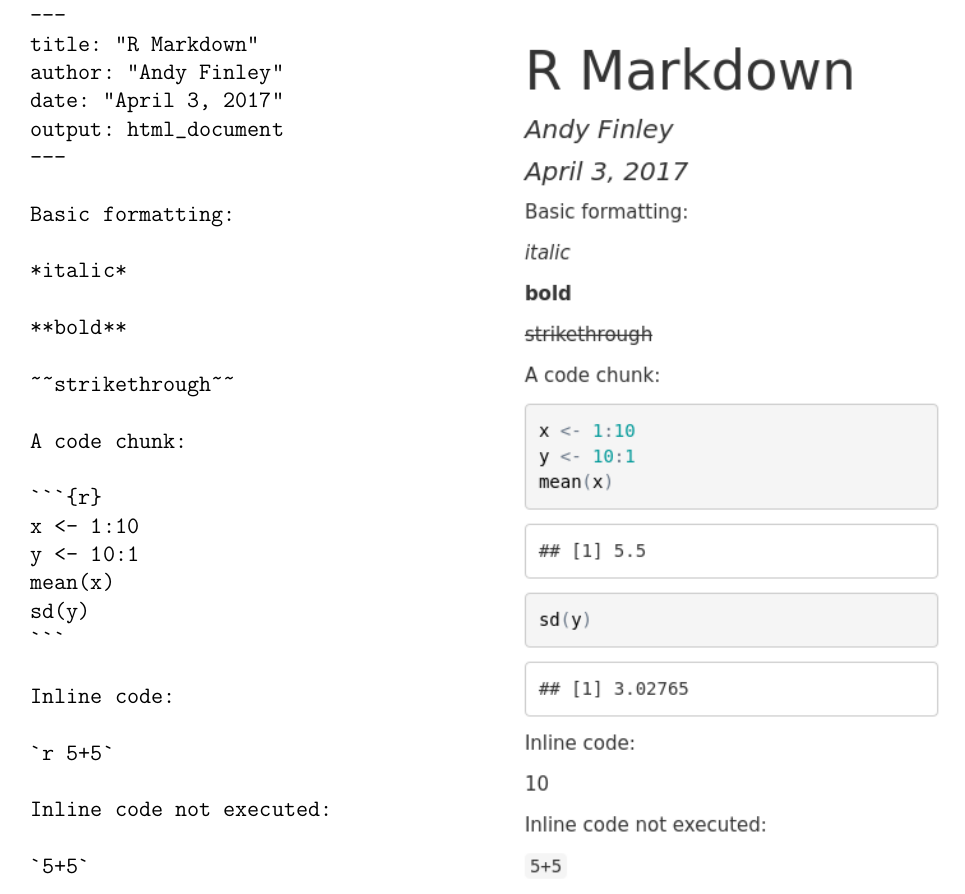
\includegraphics[width=1\linewidth]{03-scripts/03-images/rmarkdownInputOutput} 

}

\caption{Example R Markdown Input and Output}\label{fig:rmark}
\end{figure}

At the top of the input R Markdown file are some lines with
\texttt{-\/-\/-} at the top and the bottom. These lines are not needed,
but give a convenient way to specify the title, author, and date of the
article that are then typeset prominently at the top of the output
document. For now, don't be concerned with the lines following
\texttt{output:}. These can be omitted (or included as shown).

Next are a few lines showing some of the ways that font effects such as
italics, boldface, and strikethrough can be achieved. For example, an
asterisk before and after text sets the text in \emph{italics}, and two
asterisks before and after text sets the text in \textbf{boldface}.

More important for our purposes is the ability to include R code in the
R Markdown file, which will be executed with the output appearing in the
output document. Bits of R code included this way are called \emph{code
chunks}. The beginning of a code chunk is indicated with three backticks
and an ``r'' in curly braces:
\texttt{\textasciigrave{}\textasciigrave{}\textasciigrave{}\{r\}}. The
end of a code chunk is indicated with three backticks
\texttt{\textasciigrave{}\textasciigrave{}\textasciigrave{}}. For
example, the R Markdown file in Figure \ref{fig:rmark} has one code
chunk:

\begin{Shaded}
\begin{Highlighting}[]
\StringTok{```}\DataTypeTok{\{r\}}
\DataTypeTok{x = 1:10}
\DataTypeTok{y = 10:1}
\DataTypeTok{mean(x)}
\DataTypeTok{sd(y)}
\StringTok{```}
\end{Highlighting}
\end{Shaded}

In this code chunk two vectors \texttt{x} and \texttt{y} are created,
and the mean of \texttt{x} and the standard deviation of \texttt{y} are
computed. In the output in Figure \ref{fig:rmark} the R code is
reproduced, and the output of the two lines of code asking for the mean
and standard deviation is shown.

\subsection{Creating and processing R Markdown
documents}\label{creating-and-processing-r-markdown-documents}

RStudio has features which facilitate creating and processing R Markdown
documents. Choose
\texttt{File\ \textgreater{}\ New\ File\ \textgreater{}\ R\ \ Markdown...}.
In the ensuing dialog box, make sure that \texttt{Document} is
highlighted on the left, enter the title and author (if desired), and
choose the Default Output Format (HTML is good to begin). Then click OK.
A document will appear in the upper left of the RStudio window. It is an
R Markdown document, and the title and author you chose will show up,
delimited by \texttt{-\/-\/-} at the top of the document. A generic body
of the document will also be included.

For now just keep this generic document as is. To process it to create
the HTML output, click the \texttt{Knit\ HTML} button at the top of the
R Markdown window\footnote{If you hover your mouse over this Knit button
  after a couple seconds it should display a keyboard shortcut for you
  to do this if you don't like pushing buttons}. You'll be prompted to
choose a filename for the R Markdown file. Make sure that you use
\texttt{.Rmd} as the extension for this file. Once you've successfully
saved the file, RStudio will process the file, create the HTML output,
and open this output in a new window. The HTML output file will also be
saved to your working directory. This file can be shared with others,
who can open it using a web browser such as Chrome or Firefox.

There are many options which allow customization of R Markdown
documents. Some of these affect formatting of text in the document,
while others affect how R code is evaluated and displayed. The RStudio
web site contains a useful summary of many R Markdown options at
\url{https://www.rstudio.com/wp-content/uploads/2015/03/rmarkdown-reference.pdf}.
A different, but mind-numbingly busy, cheatsheet is at
\url{https://www.rstudio.com/wp-content/uploads/2016/03/rmarkdown-cheatsheet-2.0.pdf}.
Some of the more commonly used R Markdown options are described next.

\subsection{Text: Lists and Headers}\label{text-lists-and-headers}

Unordered (sometimes called bulleted) lists and ordered lists are easy
in R Markdown. Figure \ref{fig:lists} illustrates the creation of
unordered and ordered lists.

\begin{figure}

{\centering 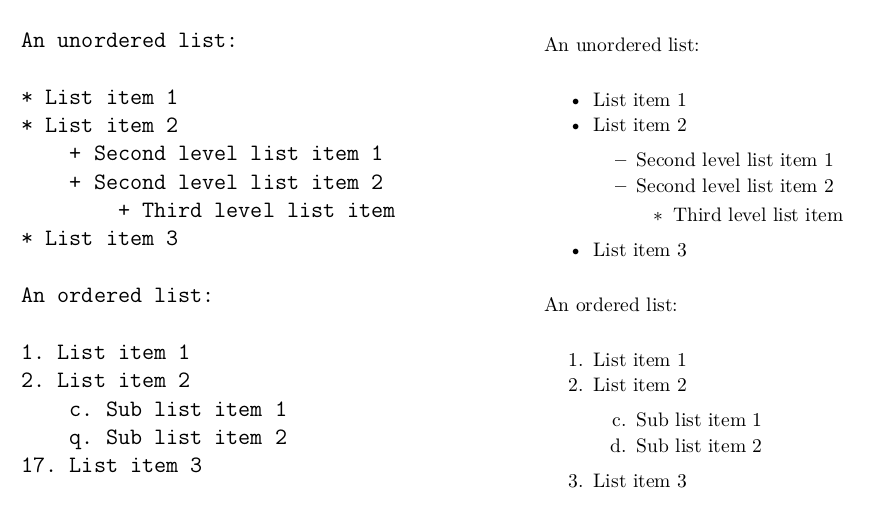
\includegraphics[width=1\linewidth]{03-scripts/03-images/listsPic} 

}

\caption{Producing Lists in R Markdown}\label{fig:lists}
\end{figure}

\begin{itemize}
\item
  For an unordered list, either an asterisk, a plus sign, or a minus
  sign may precede list items. Use a space after these symbols before
  including the list text. To have second-level items (sub-lists) indent
  four spaces before indicating the list item. This can also be done for
  third-level items.
\item
  For an ordered list use a numeral followed by a period and a space (1.
  or 2. or 3. or \ldots{}) to indicate a numbered list, and use a letter
  followed by a period and a space (a. or b. or c. or \ldots{}) to
  indicate a lettered list. The same four space convention used in
  unordered lists is used to designate ordered sub lists.
\item
  For an ordered list, the first list item will be labeled with the
  number or letter that you specify, but subsequent list items will be
  numbered sequentially. The example in Figure \ref{fig:lists} will make
  this more clear. In those examples notice that for the ordered list,
  although the first-level numbers given in the R Markdown file are 1,
  2, and 17, the numbers printed in the output are 1, 2, and 3.
  Similarly the letters given in the R Markdown file are c and q, but
  the output file prints c and d.
\end{itemize}

R Markdown does not give substantial control over font size. Different
``header'' levels are available that provide different font sizes. Put
one or more hash marks in front of text to specify different header
levels. Other font choices such as subscripts and superscripts are
possible, by surrounding the text either by tildes or carets. More
sophisticated mathematical displays are also possible, and are
surrounded by dollar signs. The actual mathematical expressions are
specified using a language called LaTeX See Figures \ref{fig:headers}
and \ref{fig:latex} for examples.

\begin{figure}

{\centering 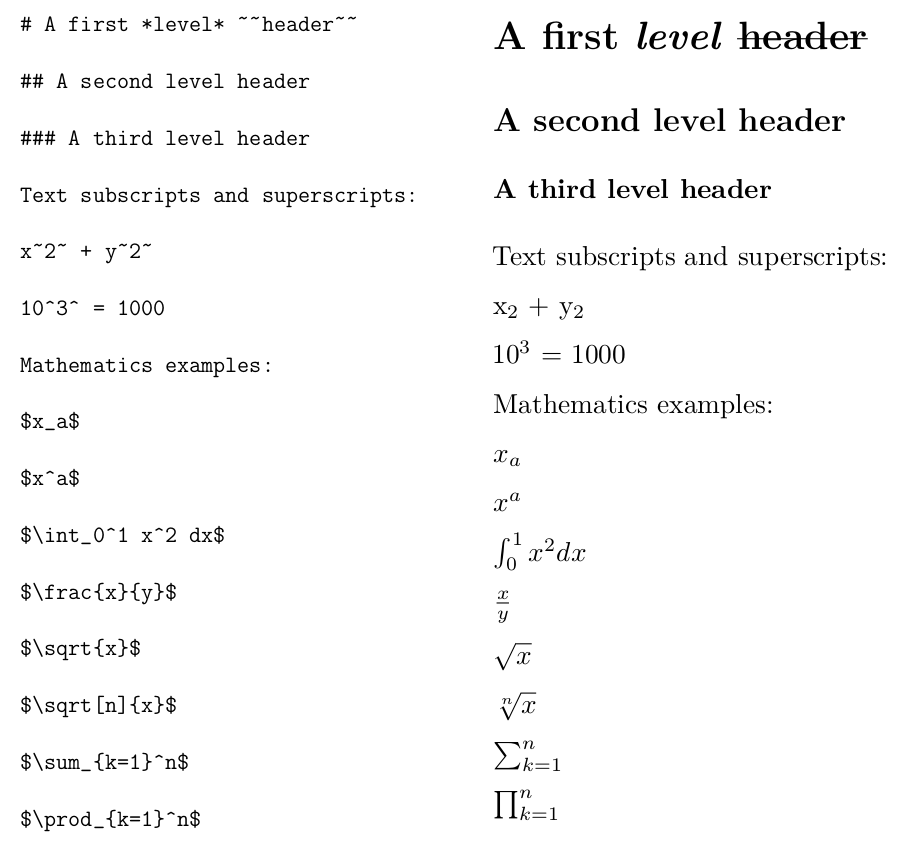
\includegraphics[width=1\linewidth]{03-scripts/03-images/headersAndLatex} 

}

\caption{Headers and Some LaTeX in R Markdown}\label{fig:headers}
\end{figure}

\begin{figure}

{\centering 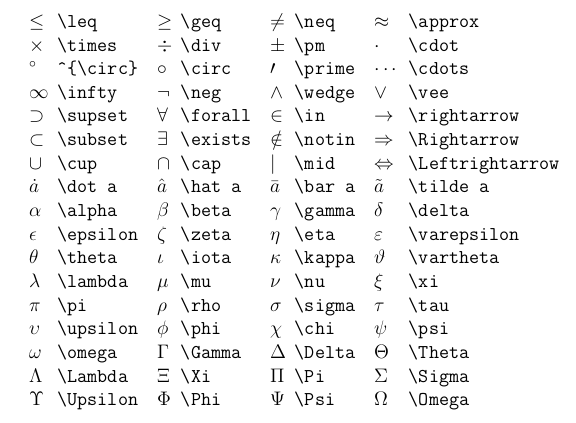
\includegraphics[width=1\linewidth]{03-scripts/03-images/latex} 

}

\caption{Other useful LaTeX symbols and expressions in R Markdown}\label{fig:latex}
\end{figure}

\subsection{Code Chunks}\label{code-chunks}

R Markdown provides a large number of options to vary the behavior of
code chunks. In some contexts it is useful to display the output but not
the R code leading to the output. In some contexts it is useful to
display the R prompt, while in others it is not. Maybe we want to change
the size of figures created by graphics commands. And so on. A large
number of code chunk options are described in
\url{http://www.rstudio.com/wp-content/uploads/2015/03/rmarkdown-reference.pdf}.

Code chunk options are specified in the curly braces near the beginning
of a code chunk. Below are a few of the more commonly used options are
described. The use of these options is illustrated in Figure
\ref{fig:chunk}.

\begin{enumerate}
\def\labelenumi{\arabic{enumi}.}
\item
  \texttt{echo=FALSE} specifies that the R code itself should not be
  printed, but any output of the R code should be printed in the
  resulting document.
\item
  \texttt{include=FALSE} specifies that neither the R code nor the
  output should be printed. However, the objects created by the code
  chunk will be available for use in later code chunks.
\item
  \texttt{eval=FALSE} specifies that the R code should not be evaluated.
  The code will be printed unless, for example, \texttt{echo=FALSE} is
  also given as an option.
\item
  \texttt{error=FALSE} and \texttt{warning=FALSE} specify that,
  respectively, error messages and warning messages generated by the R
  code should not be printed.
\item
  The \texttt{comment} option allows a specified character string to be
  prepended to each line of results. By default this is set to
  \texttt{comment\ =\ \textquotesingle{}\#\#\textquotesingle{}} which
  explains the two hash marks preceding the results in Figure
  \ref{fig:rmark}. Setting \texttt{comment\ =\ NA} presents output
  without any character string prepended. That is done in most code
  chunks in this book.
\item
  \texttt{prompt=TRUE} specifies that the R prompt
  \texttt{\textgreater{}} will be prepended to each line of R code shown
  in the document. \texttt{prompt\ =\ FALSE} specifies that command
  prompts should not be included.
\item
  \texttt{fig.height} and \texttt{fig.width} specify the height and
  width of figures generated by R code. These are specified in inches.
  For example, \texttt{fig.height=4} specifies a four inch high figure.
\end{enumerate}

Figures \ref{fig:chunk} gives examples of the use of code chunk options.

\begin{figure}

{\centering 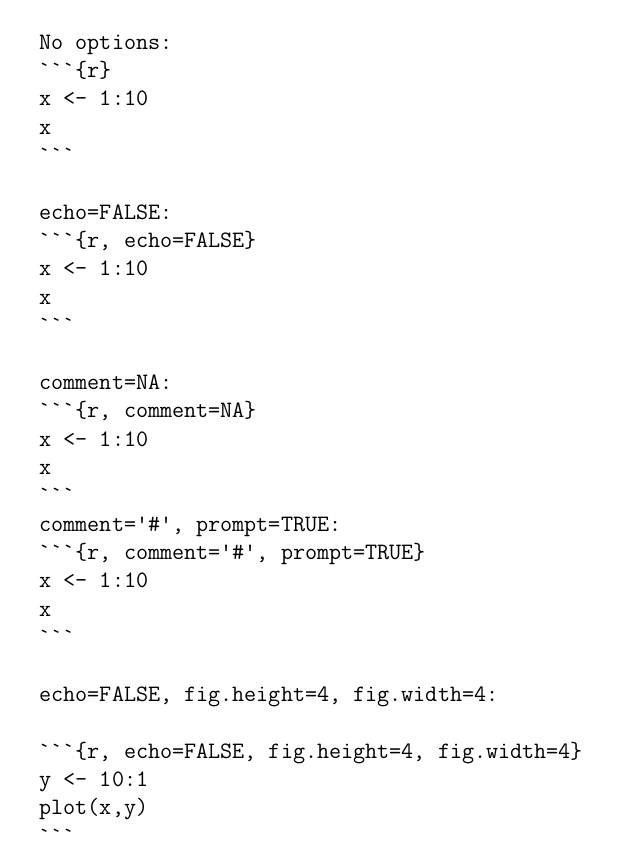
\includegraphics[width=0.5\linewidth]{03-scripts/03-images/chunks1} 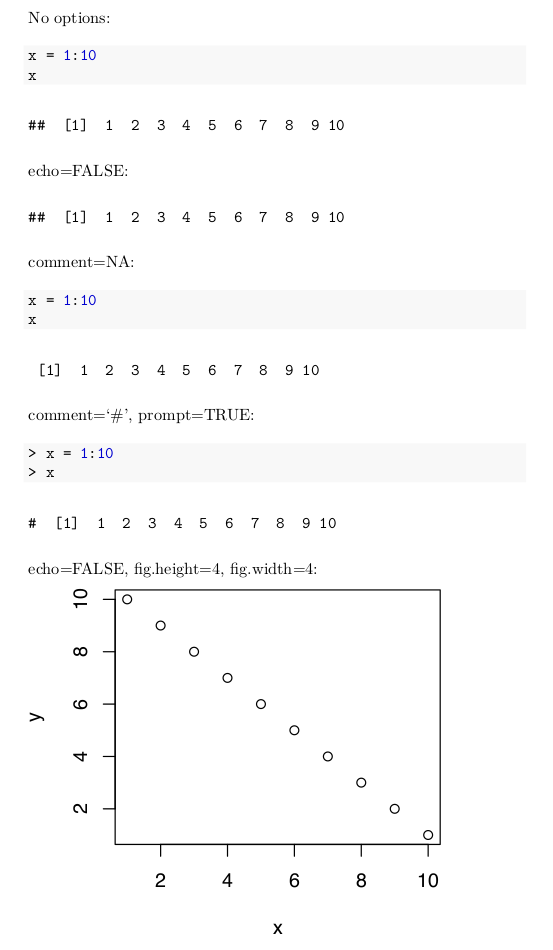
\includegraphics[width=0.5\linewidth]{03-scripts/03-images/chunks2} 

}

\caption{Output of Example R Markdown}\label{fig:chunk}
\end{figure}

\subsection{Output formats other than
HTML}\label{output-formats-other-than-html}

It is possible to use R Markdown to produce documents in formats other
than HTML, including Word and PDF documents. Next to the
\texttt{Knit\ HTML} button is a down arrow. Click on this and choose
\texttt{Knit\ Word} to produce a Microsoft word output document.
Although there is also a \texttt{Knit\ PDF} button, PDF output requires
additional software called TeX in addition to RStudio.\footnote{It isn't
  particularly hard to install TeX software. For a Microsoft Windows
  system, MiKTeX is convenient and is available from
  \url{https://miktex.org}. For a Mac system, MacTeX is available from
  \url{https://www.tug.org/mactex/}}

\subsection{LaTeX, knitr, and bookdown}\label{latex-knitr-and-bookdown}

While R Markdown provides substantial flexibility and power, it lacks
features such as cross-referencing, fine control over fonts, etc. If
this is desired, a variant of R Markdown called \texttt{knitr}, which
has very similar syntax to R Markdown for code chunks, can be used in
conjunction with the typesetting system LaTeX to produce documents. We
originally created this book using knitr and LaTeX. For simpler tasks,
however, R Markdown is sufficient, and substantially easier to learn.

As you know (since you are reading this) we are currently converting
this book into R Markdown using the package \texttt{bookdown} written by
Yihui Xie. This package utilizes the R Markdown style that is described
above, and also incorporates numerous other features that R Markdown
alone does not have (see the previous paragraph). Perhaps the best part
about \texttt{bookdown} (in addition to it's lovely formatting style) is
that we can make it interactive, so as you read the html version of this
book you can interact with the code itself. You will experience this
first hand when you work through the spatial data and databases
chapters.

\chapter{Data Structures}\label{data-structures}

A data structure is a format for organizing and storing data. The
structure is designed so that data can be accessed and worked with in
specific ways. Statistical software and programming languages have
methods (or functions) designed to operate on different kinds of data
structures.

This chapter's focus is on data structures. To help initial
understanding, the data in this chapter will be relatively modest in
size and complexity. The ideas and methods, however, generalize to
larger and more complex data sets.

The base data structures in R are vectors, matrices, arrays, data
frames, and lists. The first three, vectors, matrices, and arrays, are
\emph{homogeneous}, meaning that all elements are required to be of the
same type (e.g., all numeric or all character). Data frames and lists
are \emph{heterogeneous}, allowing elements to be of different types
(e.g., some elements of a data frame may be numeric while other elements
may be character). These base structures can also be organized by their
dimensionality, as shown in Table \ref{tab:dataStructures}.

\begin{table}

\caption{\label{tab:dataStructures}Dimension and Type Content of Base Data Structures in R.}
\centering
\begin{tabular}[t]{lll}
\toprule
Dimension & Homogeneous & Heterogeneous\\
\midrule
1 & Atomic Vector & List\\
2 & Matrix & Data Frame\\
N & Array & \\
\bottomrule
\end{tabular}
\end{table}

R has no scalar types (0-dimensional). Individual numbers or strings are
actually vectors of length one.

An efficient way to understand what comprises a given object is to use
the \texttt{str()} function. \texttt{str()} is short for structure and
prints a compact, human-readable description of any R data structure.
For example, in the code below, we prove to ourselves that what we might
think of as a scalar value is actually a vector of length one.

\begin{Shaded}
\begin{Highlighting}[]
\OperatorTok{>}\StringTok{ }\NormalTok{a <-}\StringTok{ }\DecValTok{1}
\OperatorTok{>}\StringTok{ }\KeywordTok{str}\NormalTok{(a)}
\end{Highlighting}
\end{Shaded}

\begin{verbatim}
 num 1
\end{verbatim}

\begin{Shaded}
\begin{Highlighting}[]
\OperatorTok{>}\StringTok{ }\KeywordTok{is.vector}\NormalTok{(a)}
\end{Highlighting}
\end{Shaded}

\begin{verbatim}
[1] TRUE
\end{verbatim}

\begin{Shaded}
\begin{Highlighting}[]
\OperatorTok{>}\StringTok{ }\KeywordTok{length}\NormalTok{(a)}
\end{Highlighting}
\end{Shaded}

\begin{verbatim}
[1] 1
\end{verbatim}

Here we assigned \texttt{a} the scalar value one. The \texttt{str(a)}
prints \texttt{num\ 1}, which says \texttt{a} is numeric of length one.
Then just to be sure we used the function \texttt{is.vector()} to test
if \texttt{a} is in fact a vector. Then, just for fun, we computed the
length of \texttt{a} which again returns one. There are a set of similar
logical tests for the other base data structures, e.g.,
\texttt{is.matrix()}, \texttt{is.array()}, \texttt{is.data.frame()}, and
\texttt{is.list()}. These will all come in handy as we encounter
different R objects.

\section{Vectors}\label{vectors}

Think of a vector\footnote{Technically the objects described in this
  section are ``atomic'' vectors (all elements of the same type), since
  lists are also actually vectors. This will not be an important issue
  in this course, and the shorter term vector will be used for atomic
  vectors.} as a structure to represent one variable in a data set. For
example a vector might hold the DBH, in inches, of six trees in a data
set, and another vector might hold the species of those six trees. The
\texttt{c()} function in R is useful for creating vectors and for
modifying existing vectors. Think of \texttt{c} as standing for
``combine''" or ``concatenate.''

\begin{Shaded}
\begin{Highlighting}[]
\OperatorTok{>}\StringTok{ }\NormalTok{dbh <-}\StringTok{ }\KeywordTok{c}\NormalTok{(}\DecValTok{20}\NormalTok{, }\DecValTok{18}\NormalTok{, }\DecValTok{13}\NormalTok{, }\DecValTok{16}\NormalTok{, }\DecValTok{10}\NormalTok{, }\DecValTok{14}\NormalTok{)}
\OperatorTok{>}\StringTok{ }\NormalTok{dbh}
\end{Highlighting}
\end{Shaded}

\begin{verbatim}
[1] 20 18 13 16 10 14
\end{verbatim}

\begin{Shaded}
\begin{Highlighting}[]
\OperatorTok{>}\StringTok{ }\NormalTok{spp <-}\StringTok{ }\KeywordTok{c}\NormalTok{(}\StringTok{"Acer rubrum"}\NormalTok{, }\StringTok{"Acer rubrum"}\NormalTok{, }\StringTok{"Betula lenta"}\NormalTok{, }\StringTok{"Betula lenta"}\NormalTok{, }
\OperatorTok{+}\StringTok{          "Prunus serotina"}\NormalTok{, }\StringTok{"Prunus serotina"}\NormalTok{)}
\OperatorTok{>}\StringTok{ }\NormalTok{spp}
\end{Highlighting}
\end{Shaded}

\begin{verbatim}
[1] "Acer rubrum"     "Acer rubrum"    
[3] "Betula lenta"    "Betula lenta"   
[5] "Prunus serotina" "Prunus serotina"
\end{verbatim}

Notice that elements of a vector are separated by commas when using the
\texttt{c()} function to create a vector. Also notice that character
values are placed inside quotation marks.

The \texttt{c()} function also can be used to add to an existing vector.
For example, if a seventh tree were included in the data set, and its
DBH was 13 inches, the existing vectors could be modified as follows.

\begin{Shaded}
\begin{Highlighting}[]
\OperatorTok{>}\StringTok{ }\NormalTok{dbh <-}\StringTok{ }\KeywordTok{c}\NormalTok{(dbh, }\DecValTok{13}\NormalTok{)}
\OperatorTok{>}\StringTok{ }\NormalTok{spp <-}\StringTok{ }\KeywordTok{c}\NormalTok{(spp, }\StringTok{"Acer rubrum"}\NormalTok{)}
\OperatorTok{>}\StringTok{ }\NormalTok{dbh}
\end{Highlighting}
\end{Shaded}

\begin{verbatim}
[1] 20 18 13 16 10 14 13
\end{verbatim}

\begin{Shaded}
\begin{Highlighting}[]
\OperatorTok{>}\StringTok{ }\NormalTok{spp}
\end{Highlighting}
\end{Shaded}

\begin{verbatim}
[1] "Acer rubrum"     "Acer rubrum"    
[3] "Betula lenta"    "Betula lenta"   
[5] "Prunus serotina" "Prunus serotina"
[7] "Acer rubrum"    
\end{verbatim}

\subsection{Types, Conversion, and
Coercion}\label{types-conversion-and-coercion}

Clearly it is important to distinguish between different types of
vectors. For example, it makes sense to ask R to calculate the mean of
the DBH stored in \texttt{dbh}, but does not make sense to ask R to
compute the mean of the species stored in \texttt{spp}. Vectors in R may
have one of six different ``types'': character, double, integer,
logical, complex, and raw. Only the first four of these will be of
interest below, and the distinction between double and integer will not
be of great import. To illustrate logical vectors, imagine the field
technician who measured the trees also indicated if the tree was
acceptable growing stock (\texttt{ags}) and the call was coded as TRUE
if the tree was acceptable and FALSE if the tree was not acceptable.

\begin{Shaded}
\begin{Highlighting}[]
\OperatorTok{>}\StringTok{ }\KeywordTok{typeof}\NormalTok{(dbh)}
\end{Highlighting}
\end{Shaded}

\begin{verbatim}
[1] "double"
\end{verbatim}

\begin{Shaded}
\begin{Highlighting}[]
\OperatorTok{>}\StringTok{ }\KeywordTok{typeof}\NormalTok{(spp)}
\end{Highlighting}
\end{Shaded}

\begin{verbatim}
[1] "character"
\end{verbatim}

\begin{Shaded}
\begin{Highlighting}[]
\OperatorTok{>}\StringTok{ }\NormalTok{ags <-}\StringTok{ }\KeywordTok{c}\NormalTok{(}\OtherTok{TRUE}\NormalTok{, }\OtherTok{TRUE}\NormalTok{, }\OtherTok{FALSE}\NormalTok{, }\OtherTok{TRUE}\NormalTok{, }\OtherTok{FALSE}\NormalTok{, }\OtherTok{FALSE}\NormalTok{, }\OtherTok{TRUE}\NormalTok{)}
\OperatorTok{>}\StringTok{ }\NormalTok{ags}
\end{Highlighting}
\end{Shaded}

\begin{verbatim}
[1]  TRUE  TRUE FALSE  TRUE FALSE FALSE  TRUE
\end{verbatim}

\begin{Shaded}
\begin{Highlighting}[]
\OperatorTok{>}\StringTok{ }\KeywordTok{typeof}\NormalTok{(ags)}
\end{Highlighting}
\end{Shaded}

\begin{verbatim}
[1] "logical"
\end{verbatim}

It may be surprising to see the DBH variable \texttt{dbh} is of type
\texttt{double}, even though its values are all integers. By default R
creates a double type vector when numeric values are given via the
\texttt{c()} function.

When it makes sense, it is possible to convert vectors to a different
type. Consider the following examples.

\begin{Shaded}
\begin{Highlighting}[]
\OperatorTok{>}\StringTok{ }\NormalTok{dbh.int <-}\StringTok{ }\KeywordTok{as.integer}\NormalTok{(dbh)}
\OperatorTok{>}\StringTok{ }\NormalTok{dbh.int}
\end{Highlighting}
\end{Shaded}

\begin{verbatim}
[1] 20 18 13 16 10 14 13
\end{verbatim}

\begin{Shaded}
\begin{Highlighting}[]
\OperatorTok{>}\StringTok{ }\KeywordTok{typeof}\NormalTok{(dbh.int)}
\end{Highlighting}
\end{Shaded}

\begin{verbatim}
[1] "integer"
\end{verbatim}

\begin{Shaded}
\begin{Highlighting}[]
\OperatorTok{>}\StringTok{ }\NormalTok{dbh.char <-}\StringTok{ }\KeywordTok{as.character}\NormalTok{(dbh)}
\OperatorTok{>}\StringTok{ }\NormalTok{dbh.char}
\end{Highlighting}
\end{Shaded}

\begin{verbatim}
[1] "20" "18" "13" "16" "10" "14" "13"
\end{verbatim}

\begin{Shaded}
\begin{Highlighting}[]
\OperatorTok{>}\StringTok{ }\NormalTok{ags.double <-}\StringTok{ }\KeywordTok{as.double}\NormalTok{(ags)}
\OperatorTok{>}\StringTok{ }\NormalTok{ags.double}
\end{Highlighting}
\end{Shaded}

\begin{verbatim}
[1] 1 1 0 1 0 0 1
\end{verbatim}

\begin{Shaded}
\begin{Highlighting}[]
\OperatorTok{>}\StringTok{ }\NormalTok{spp.oops <-}\StringTok{ }\KeywordTok{as.double}\NormalTok{(spp)}
\end{Highlighting}
\end{Shaded}

\begin{verbatim}
Warning: NAs introduced by coercion
\end{verbatim}

\begin{Shaded}
\begin{Highlighting}[]
\OperatorTok{>}\StringTok{ }\NormalTok{spp.oops}
\end{Highlighting}
\end{Shaded}

\begin{verbatim}
[1] NA NA NA NA NA NA NA
\end{verbatim}

\begin{Shaded}
\begin{Highlighting}[]
\OperatorTok{>}\StringTok{ }\KeywordTok{sum}\NormalTok{(ags)}
\end{Highlighting}
\end{Shaded}

\begin{verbatim}
[1] 4
\end{verbatim}

The integer version of \texttt{dbh} doesn't look any different, but it
is stored differently, which can be important both for computational
efficiency and for interfacing with other languages such as C++. As
noted above, however, we will not worry about the distinction between
integer and double types. Converting \texttt{dbh} to character goes as
expected---the character representation of the numbers replace the
numbers themselves. Converting the logical vector \texttt{ags} to double
is pretty straightforward too---\texttt{FALSE} is converted to zero, and
\texttt{TRUE} is converted to one. Now think about converting the
character vector \texttt{spp} to a numeric double vector. It's not at
all clear how to represent ``Acer rubrum'' as a number. In fact in this
case what R does is to create a double vector, but with each element set
to \texttt{NA}, which is the representation of missing data \footnote{Missing
  data will be discussed in more detail later in the chapter.}. Finally
consider the code \texttt{sum(ags)}. Now \texttt{ags} is a logical
vector, but when R sees that we are asking to sum this logical vector,
it automatically converts it to a numerical vector and then adds the
zeros and ones representing FALSE and TRUE.

R also has functions to test whether a vector is of a particular type.

\begin{Shaded}
\begin{Highlighting}[]
\OperatorTok{>}\StringTok{ }\KeywordTok{is.double}\NormalTok{(dbh)}
\end{Highlighting}
\end{Shaded}

\begin{verbatim}
[1] TRUE
\end{verbatim}

\begin{Shaded}
\begin{Highlighting}[]
\OperatorTok{>}\StringTok{ }\KeywordTok{is.character}\NormalTok{(dbh)}
\end{Highlighting}
\end{Shaded}

\begin{verbatim}
[1] FALSE
\end{verbatim}

\begin{Shaded}
\begin{Highlighting}[]
\OperatorTok{>}\StringTok{ }\KeywordTok{is.integer}\NormalTok{(dbh.int)}
\end{Highlighting}
\end{Shaded}

\begin{verbatim}
[1] TRUE
\end{verbatim}

\begin{Shaded}
\begin{Highlighting}[]
\OperatorTok{>}\StringTok{ }\KeywordTok{is.logical}\NormalTok{(ags)}
\end{Highlighting}
\end{Shaded}

\begin{verbatim}
[1] TRUE
\end{verbatim}

\subsubsection{Coercion}\label{coercion}

Consider the following examples.

\begin{Shaded}
\begin{Highlighting}[]
\OperatorTok{>}\StringTok{ }\NormalTok{xx <-}\StringTok{ }\KeywordTok{c}\NormalTok{(}\DecValTok{1}\NormalTok{, }\DecValTok{2}\NormalTok{, }\DecValTok{3}\NormalTok{, }\OtherTok{TRUE}\NormalTok{)}
\OperatorTok{>}\StringTok{ }\NormalTok{xx}
\end{Highlighting}
\end{Shaded}

\begin{verbatim}
[1] 1 2 3 1
\end{verbatim}

\begin{Shaded}
\begin{Highlighting}[]
\OperatorTok{>}\StringTok{ }\NormalTok{yy <-}\StringTok{ }\KeywordTok{c}\NormalTok{(}\DecValTok{1}\NormalTok{, }\DecValTok{2}\NormalTok{, }\DecValTok{3}\NormalTok{, }\StringTok{"dog"}\NormalTok{)}
\OperatorTok{>}\StringTok{ }\NormalTok{yy}
\end{Highlighting}
\end{Shaded}

\begin{verbatim}
[1] "1"   "2"   "3"   "dog"
\end{verbatim}

\begin{Shaded}
\begin{Highlighting}[]
\OperatorTok{>}\StringTok{ }\NormalTok{zz <-}\StringTok{ }\KeywordTok{c}\NormalTok{(}\OtherTok{TRUE}\NormalTok{, }\OtherTok{FALSE}\NormalTok{, }\StringTok{"cat"}\NormalTok{)}
\OperatorTok{>}\StringTok{ }\NormalTok{zz}
\end{Highlighting}
\end{Shaded}

\begin{verbatim}
[1] "TRUE"  "FALSE" "cat"  
\end{verbatim}

\begin{Shaded}
\begin{Highlighting}[]
\OperatorTok{>}\StringTok{ }\NormalTok{dbh }\OperatorTok{+}\StringTok{ }\NormalTok{ags}
\end{Highlighting}
\end{Shaded}

\begin{verbatim}
[1] 21 19 13 17 10 14 14
\end{verbatim}

Vectors in R can only contain elements of one type. If more than one
type is included in a \texttt{c()} function, R silently \emph{coerces}
the vector to be of one type. The examples illustrate the hierarchy---if
any element is a character, then the whole vector is character. If some
elements are numeric (either integer or double) and other elements are
logical, then the whole vector is numeric. Note what happened when R was
asked to add the numeric vector \texttt{dbh} to the logical vector
\texttt{ags}. The logical vector was silently coerced to be numeric, so
that FALSE became zero and TRUE became one, and then the two numeric
vectors were added.

\subsection{Accessing Specific Elements of
Vectors}\label{accessing-specific-elements-of-vectors}

To access and possibly change specific elements of vectors, refer to the
position of the element in square brackets. For example,
\texttt{dbh{[}4{]}} refers to the fourth element of the vector
\texttt{dbh}. Note that R starts the numbering of elements at 1, i.e.,
the first element of a vector \texttt{x} is \texttt{x{[}1{]}}.

\begin{Shaded}
\begin{Highlighting}[]
\OperatorTok{>}\StringTok{ }\NormalTok{dbh}
\end{Highlighting}
\end{Shaded}

\begin{verbatim}
[1] 20 18 13 16 10 14 13
\end{verbatim}

\begin{Shaded}
\begin{Highlighting}[]
\OperatorTok{>}\StringTok{ }\NormalTok{dbh[}\DecValTok{5}\NormalTok{]}
\end{Highlighting}
\end{Shaded}

\begin{verbatim}
[1] 10
\end{verbatim}

\begin{Shaded}
\begin{Highlighting}[]
\OperatorTok{>}\StringTok{ }\NormalTok{dbh[}\DecValTok{1}\OperatorTok{:}\DecValTok{3}\NormalTok{]}
\end{Highlighting}
\end{Shaded}

\begin{verbatim}
[1] 20 18 13
\end{verbatim}

\begin{Shaded}
\begin{Highlighting}[]
\OperatorTok{>}\StringTok{ }\KeywordTok{length}\NormalTok{(dbh)}
\end{Highlighting}
\end{Shaded}

\begin{verbatim}
[1] 7
\end{verbatim}

\begin{Shaded}
\begin{Highlighting}[]
\OperatorTok{>}\StringTok{ }\NormalTok{dbh[}\KeywordTok{length}\NormalTok{(dbh)]}
\end{Highlighting}
\end{Shaded}

\begin{verbatim}
[1] 13
\end{verbatim}

\begin{Shaded}
\begin{Highlighting}[]
\OperatorTok{>}\StringTok{ }\NormalTok{dbh[]}
\end{Highlighting}
\end{Shaded}

\begin{verbatim}
[1] 20 18 13 16 10 14 13
\end{verbatim}

\begin{Shaded}
\begin{Highlighting}[]
\OperatorTok{>}\StringTok{ }\NormalTok{dbh[}\DecValTok{3}\NormalTok{] <-}\StringTok{ }\DecValTok{202}\NormalTok{  ##crazy big tree}
\OperatorTok{>}\StringTok{ }\NormalTok{dbh}
\end{Highlighting}
\end{Shaded}

\begin{verbatim}
[1]  20  18 202  16  10  14  13
\end{verbatim}

\begin{Shaded}
\begin{Highlighting}[]
\OperatorTok{>}\StringTok{ }\NormalTok{dbh[}\DecValTok{1}\OperatorTok{:}\DecValTok{3}\NormalTok{] <-}\StringTok{ }\KeywordTok{c}\NormalTok{(}\DecValTok{16}\NormalTok{, }\DecValTok{8}\NormalTok{, }\DecValTok{2}\NormalTok{)}
\OperatorTok{>}\StringTok{ }\NormalTok{dbh}
\end{Highlighting}
\end{Shaded}

\begin{verbatim}
[1] 16  8  2 16 10 14 13
\end{verbatim}

Note that including nothing in the square brackets results in the whole
vector being returned. We can also assign values to vectors by accessing
the position(s) where the new values will be assigned. For example, in
the above code chunk \texttt{dbh{[}3{]}} is changed to 202, then the
values in the first three elements of \texttt{dbh} are changed to 10, 8,
and 2, respectively.

Negative numbers in the square brackets tell R to omit the corresponding
value. And a zero as a subscript returns nothing (more precisely, it
returns a length zero vector of the appropriate type).

\begin{Shaded}
\begin{Highlighting}[]
\OperatorTok{>}\StringTok{ }\NormalTok{dbh[}\OperatorTok{-}\DecValTok{3}\NormalTok{]}
\end{Highlighting}
\end{Shaded}

\begin{verbatim}
[1] 16  8 16 10 14 13
\end{verbatim}

\begin{Shaded}
\begin{Highlighting}[]
\OperatorTok{>}\StringTok{ }\NormalTok{dbh[}\OperatorTok{-}\KeywordTok{length}\NormalTok{(dbh)]}
\end{Highlighting}
\end{Shaded}

\begin{verbatim}
[1] 16  8  2 16 10 14
\end{verbatim}

\begin{Shaded}
\begin{Highlighting}[]
\OperatorTok{>}\StringTok{ }\NormalTok{fewer.dbh <-}\StringTok{ }\NormalTok{dbh[}\OperatorTok{-}\KeywordTok{c}\NormalTok{(}\DecValTok{1}\NormalTok{, }\DecValTok{3}\NormalTok{, }\DecValTok{5}\NormalTok{)]}
\OperatorTok{>}\StringTok{ }\NormalTok{fewer.dbh}
\end{Highlighting}
\end{Shaded}

\begin{verbatim}
[1]  8 16 14 13
\end{verbatim}

\begin{Shaded}
\begin{Highlighting}[]
\OperatorTok{>}\StringTok{ }\NormalTok{dbh[}\DecValTok{0}\NormalTok{]}
\end{Highlighting}
\end{Shaded}

\begin{verbatim}
numeric(0)
\end{verbatim}

\begin{Shaded}
\begin{Highlighting}[]
\OperatorTok{>}\StringTok{ }\NormalTok{dbh[}\KeywordTok{c}\NormalTok{(}\DecValTok{0}\NormalTok{, }\DecValTok{2}\NormalTok{, }\DecValTok{1}\NormalTok{)]}
\end{Highlighting}
\end{Shaded}

\begin{verbatim}
[1]  8 16
\end{verbatim}

\begin{Shaded}
\begin{Highlighting}[]
\OperatorTok{>}\StringTok{ }\NormalTok{dbh[}\KeywordTok{c}\NormalTok{(}\OperatorTok{-}\DecValTok{1}\NormalTok{, }\DecValTok{2}\NormalTok{)]}
\end{Highlighting}
\end{Shaded}

\begin{verbatim}
Error in dbh[c(-1, 2)]: only 0's may be mixed with negative subscripts
\end{verbatim}

Note that mixing zero and other nonzero subscripts is allowed, but
mixing negative and positive subscripts is not allowed.

What about the (usual) case where we don't know the positions of the
elements we want? For example possibly we want the DBH of all acceptable
growing stock trees in the data. Later we will learn how to subset using
logical indices, which is a very powerful way to access desired elements
of a vector \footnote{We had a prelude to this in the temperature data
  exercise.}.

\section{Factors}\label{factors}

Categorical variables such as \texttt{spp} can be represented as
character vectors. In many cases this simple representation is
sufficient. Consider, however, two other categorical variables, one
representing crown class \texttt{S}, \texttt{I}, \texttt{C}, and
\texttt{D} (i.e., \textbf{S}uppressed, \textbf{I}ntermediate,
\textbf{C}odominate, \textbf{D}ominant), and another representing grade
of the first log via categories \texttt{Grade\ 1}, \texttt{Grade\ 2},
and \texttt{Grade\ 3}. Suppose that for the small data set considered
here, all trees are either dominant or codominant crown class. If we
just represented the variable via a character vector, there would be no
way to know that there are two other categories, representing suppressed
and intermediate, because they happen to not be present in the data set.
In addition, for the log grade variable the character vector
representation does not explicitly indicate that there is an ordering of
the levels.

Factors in R provide a more sophisticated way to represent categorical
variables. Factors explicitly contain all possible levels, and allow
ordering of levels.

\begin{Shaded}
\begin{Highlighting}[]
\OperatorTok{>}\StringTok{ }\NormalTok{crown.class <-}\StringTok{ }\KeywordTok{c}\NormalTok{(}\StringTok{"D"}\NormalTok{, }\StringTok{"D"}\NormalTok{, }\StringTok{"C"}\NormalTok{, }\StringTok{"D"}\NormalTok{, }\StringTok{"D"}\NormalTok{, }\StringTok{"C"}\NormalTok{, }\StringTok{"C"}\NormalTok{)}
\OperatorTok{>}\StringTok{ }\NormalTok{grade <-}\StringTok{ }\KeywordTok{c}\NormalTok{(}\StringTok{"Grade 1"}\NormalTok{, }\StringTok{"Grade 1"}\NormalTok{, }\StringTok{"Grade 3"}\NormalTok{, }\StringTok{"Grade 2"}\NormalTok{, }\StringTok{"Grade 3"}\NormalTok{, }
\OperatorTok{+}\StringTok{   "Grade 3"}\NormalTok{, }\StringTok{"Grade 2"}\NormalTok{)}
\OperatorTok{>}\StringTok{ }\NormalTok{crown.class}
\end{Highlighting}
\end{Shaded}

\begin{verbatim}
[1] "D" "D" "C" "D" "D" "C" "C"
\end{verbatim}

\begin{Shaded}
\begin{Highlighting}[]
\OperatorTok{>}\StringTok{ }\NormalTok{grade}
\end{Highlighting}
\end{Shaded}

\begin{verbatim}
[1] "Grade 1" "Grade 1" "Grade 3" "Grade 2" "Grade 3"
[6] "Grade 3" "Grade 2"
\end{verbatim}

\begin{Shaded}
\begin{Highlighting}[]
\OperatorTok{>}\StringTok{ }\NormalTok{crown.class <-}\StringTok{ }\KeywordTok{factor}\NormalTok{(crown.class, }\DataTypeTok{levels =} \KeywordTok{c}\NormalTok{(}\StringTok{"S"}\NormalTok{, }\StringTok{"I"}\NormalTok{, }
\OperatorTok{+}\StringTok{   "C"}\NormalTok{, }\StringTok{"D"}\NormalTok{))}
\OperatorTok{>}\StringTok{ }\NormalTok{crown.class}
\end{Highlighting}
\end{Shaded}

\begin{verbatim}
[1] D D C D D C C
Levels: S I C D
\end{verbatim}

\begin{Shaded}
\begin{Highlighting}[]
\OperatorTok{>}\StringTok{ }\NormalTok{grade <-}\StringTok{ }\KeywordTok{factor}\NormalTok{(grade, }\DataTypeTok{levels =} \KeywordTok{c}\NormalTok{(}\StringTok{"Grade 1"}\NormalTok{, }\StringTok{"Grade 2"}\NormalTok{, }
\OperatorTok{+}\StringTok{   "Grade 3"}\NormalTok{), }\DataTypeTok{ordered =} \OtherTok{TRUE}\NormalTok{)}
\OperatorTok{>}\StringTok{ }\NormalTok{grade}
\end{Highlighting}
\end{Shaded}

\begin{verbatim}
[1] Grade 1 Grade 1 Grade 3 Grade 2 Grade 3 Grade 3
[7] Grade 2
Levels: Grade 1 < Grade 2 < Grade 3
\end{verbatim}

In the factor version of crown class the levels are explicitly listed,
so it is clear that the two included levels are not all the possible
levels. In the factor version of log grade, the ordering is explicit as
well.

In many cases the character vector representation of a categorical
variable is sufficient and easier to work with. In this book factors
will not be used extensively. It is important to note that R often by
default creates a factor when character data are read in, and sometimes
it is necessary to use the argument \texttt{stringsAsFactors\ =\ FALSE}
to explicitly tell R not to do this. This will be seen below when data
frames are introduced.

\section{Names of objects in R}\label{names-of-objects-in-r}

Continuing the discussion about code quality from Section
\ref{quality-of-r-code}, there are a few hard and fast restrictions on
the names of objects (such as vectors) in R. Note also that there are
good practices, and things to avoid.

From the help page for \texttt{make.names} in R, the name of an R object
is ``syntactically valid'' if the name ``consists of letters, numbers
and the dot or underline characters and starts with a letter or the dot
not followed by a number'' and is not one of the ``reserved words'' in R
such as \texttt{if}, \texttt{TRUE}, \texttt{function}, etc. For example,
\texttt{c45t.le\_dog} and \texttt{.ty56} are both syntactically valid
(although not very good names) while \texttt{4DislikeCats} and
\texttt{log\#@sparty} are not.

A few important comments about naming objects follow:

\begin{enumerate}
\def\labelenumi{\arabic{enumi}.}
\tightlist
\item
  It is important to be aware that names of objects in R are
  case-sensitive, so \texttt{dbh} and \texttt{DBH} do not refer to the
  same object.
\end{enumerate}

\begin{Shaded}
\begin{Highlighting}[]
\OperatorTok{>}\StringTok{ }\NormalTok{dbh}
\end{Highlighting}
\end{Shaded}

\begin{verbatim}
[1] 16  8  2 16 10 14 13
\end{verbatim}

\begin{Shaded}
\begin{Highlighting}[]
\OperatorTok{>}\StringTok{ }\NormalTok{DBH}
\end{Highlighting}
\end{Shaded}

\begin{verbatim}
Error in eval(expr, envir, enclos): object 'DBH' not found
\end{verbatim}

\begin{enumerate}
\def\labelenumi{\arabic{enumi}.}
\setcounter{enumi}{1}
\item
  It is unwise to create an object with the same name as a built-in R
  object such as the function \texttt{c} or the function \texttt{mean}.
  In earlier versions of R this could be somewhat disastrous, but even
  in current versions, it is definitely not a good idea!
\item
  As much as possible, choose names that are informative. When creating
  a variable you may initially remember that \texttt{x} contains DBH and
  \texttt{y} contains crown class, but after a few hours, days, or
  weeks, you probably will forget this. Better options are \texttt{dbh}
  and \texttt{crown.class}.
\item
  As much as possible, be consistent in how you name objects. In
  particular, decide how to separate multi-word names. Some options
  include:

  \begin{itemize}
  \tightlist
  \item
    Using case to separate: \texttt{CrownClass} or \texttt{crownClass}
    for example
  \item
    Using underscores to separate: \texttt{crown\_class} for example
  \item
    Using a period to separate: \texttt{crown.class} for example
  \end{itemize}
\end{enumerate}

\section{Missing Data, Infinity, etc.}\label{missing-data-infinity-etc.}

Most real-world data sets have variables where some observations are
missing. In longitudinal studies of tree growth (i.e., where trees are
measured over time), it is common that trees die or cannot be located in
subsequent remeasurements. Statistical software should be able to
represent missing data and to analyze data sets in which some data are
missing.

In R, the value \texttt{NA} is used for a missing data value. Since
missing values may occur in numeric, character, and other types of data,
and since R requires that a vector contain only elements of one type,
there are different types of \texttt{NA} values. Usually R determines
the appropriate type of \texttt{NA} value automatically. It is worth
noting the default type for \texttt{NA} is logical, and that \texttt{NA}
is NOT the same as the character string \texttt{"NA"}.

\begin{Shaded}
\begin{Highlighting}[]
\OperatorTok{>}\StringTok{ }\NormalTok{missingCharacter <-}\StringTok{ }\KeywordTok{c}\NormalTok{(}\StringTok{"dog"}\NormalTok{, }\StringTok{"cat"}\NormalTok{, }\OtherTok{NA}\NormalTok{, }\StringTok{"pig"}\NormalTok{, }\OtherTok{NA}\NormalTok{, }\StringTok{"horse"}\NormalTok{)}
\OperatorTok{>}\StringTok{ }\NormalTok{missingCharacter}
\end{Highlighting}
\end{Shaded}

\begin{verbatim}
[1] "dog"   "cat"   NA      "pig"   NA      "horse"
\end{verbatim}

\begin{Shaded}
\begin{Highlighting}[]
\OperatorTok{>}\StringTok{ }\KeywordTok{is.na}\NormalTok{(missingCharacter)}
\end{Highlighting}
\end{Shaded}

\begin{verbatim}
[1] FALSE FALSE  TRUE FALSE  TRUE FALSE
\end{verbatim}

\begin{Shaded}
\begin{Highlighting}[]
\OperatorTok{>}\StringTok{ }\NormalTok{missingCharacter <-}\StringTok{ }\KeywordTok{c}\NormalTok{(missingCharacter, }\StringTok{"NA"}\NormalTok{)}
\OperatorTok{>}\StringTok{ }\NormalTok{missingCharacter}
\end{Highlighting}
\end{Shaded}

\begin{verbatim}
[1] "dog"   "cat"   NA      "pig"   NA      "horse"
[7] "NA"   
\end{verbatim}

\begin{Shaded}
\begin{Highlighting}[]
\OperatorTok{>}\StringTok{ }\KeywordTok{is.na}\NormalTok{(missingCharacter)}
\end{Highlighting}
\end{Shaded}

\begin{verbatim}
[1] FALSE FALSE  TRUE FALSE  TRUE FALSE FALSE
\end{verbatim}

\begin{Shaded}
\begin{Highlighting}[]
\OperatorTok{>}\StringTok{ }\NormalTok{allMissing <-}\StringTok{ }\KeywordTok{c}\NormalTok{(}\OtherTok{NA}\NormalTok{, }\OtherTok{NA}\NormalTok{, }\OtherTok{NA}\NormalTok{)}
\OperatorTok{>}\StringTok{ }\KeywordTok{typeof}\NormalTok{(allMissing)}
\end{Highlighting}
\end{Shaded}

\begin{verbatim}
[1] "logical"
\end{verbatim}

How should missing data be treated in computations, such as finding the
mean or standard deviation of a variable? One possibility is to return
\texttt{NA}. Another is to remove the missing value(s) and then perform
the computation.

\begin{Shaded}
\begin{Highlighting}[]
\OperatorTok{>}\StringTok{ }\KeywordTok{mean}\NormalTok{(}\KeywordTok{c}\NormalTok{(}\DecValTok{1}\NormalTok{, }\DecValTok{2}\NormalTok{, }\DecValTok{3}\NormalTok{, }\OtherTok{NA}\NormalTok{, }\DecValTok{5}\NormalTok{))}
\end{Highlighting}
\end{Shaded}

\begin{verbatim}
[1] NA
\end{verbatim}

\begin{Shaded}
\begin{Highlighting}[]
\OperatorTok{>}\StringTok{ }\KeywordTok{mean}\NormalTok{(}\KeywordTok{c}\NormalTok{(}\DecValTok{1}\NormalTok{, }\DecValTok{2}\NormalTok{, }\DecValTok{3}\NormalTok{, }\OtherTok{NA}\NormalTok{, }\DecValTok{5}\NormalTok{), }\DataTypeTok{na.rm =} \OtherTok{TRUE}\NormalTok{)}
\end{Highlighting}
\end{Shaded}

\begin{verbatim}
[1] 2.75
\end{verbatim}

As this example shows, the default behavior for the \texttt{mean()}
function is to return \texttt{NA}. If removal of the missing values and
then computing the mean is desired, the argument \texttt{na.rm} is set
to \texttt{TRUE}. Different R functions have different default
behaviors, and there are other possible actions. Consulting the help for
a function provides the details.

\subsection{Infinity and NaN}\label{infinity-and-nan}

What happens if R code requests division by zero, or results in a number
that is too large to be represented? Here are some examples.

\begin{Shaded}
\begin{Highlighting}[]
\OperatorTok{>}\StringTok{ }\NormalTok{x <-}\StringTok{ }\DecValTok{0}\OperatorTok{:}\DecValTok{4}
\OperatorTok{>}\StringTok{ }\NormalTok{x}
\end{Highlighting}
\end{Shaded}

\begin{verbatim}
[1] 0 1 2 3 4
\end{verbatim}

\begin{Shaded}
\begin{Highlighting}[]
\OperatorTok{>}\StringTok{ }\DecValTok{1}\OperatorTok{/}\NormalTok{x}
\end{Highlighting}
\end{Shaded}

\begin{verbatim}
[1]    Inf 1.0000 0.5000 0.3333 0.2500
\end{verbatim}

\begin{Shaded}
\begin{Highlighting}[]
\OperatorTok{>}\StringTok{ }\NormalTok{x}\OperatorTok{/}\NormalTok{x}
\end{Highlighting}
\end{Shaded}

\begin{verbatim}
[1] NaN   1   1   1   1
\end{verbatim}

\begin{Shaded}
\begin{Highlighting}[]
\OperatorTok{>}\StringTok{ }\NormalTok{y <-}\StringTok{ }\KeywordTok{c}\NormalTok{(}\DecValTok{10}\NormalTok{, }\DecValTok{1000}\NormalTok{, }\DecValTok{10000}\NormalTok{)}
\OperatorTok{>}\StringTok{ }\DecValTok{2}\OperatorTok{^}\NormalTok{y}
\end{Highlighting}
\end{Shaded}

\begin{verbatim}
[1]  1.024e+03 1.072e+301        Inf
\end{verbatim}

\texttt{Inf} and \texttt{-Inf} represent infinity and negative infinity
(and numbers which are too large in magnitude to be represented as
floating point numbers). \texttt{NaN} represents the result of a
calculation where the result is undefined, such as dividing zero by
zero. All of these are common to a variety of programming languages,
including R.

\section{Data Frames}\label{data-frames}

Commonly data is rectangular in form, with variables as columns and
cases as rows. Continuing with the species, DBH, and acceptable growing
stock data, each of those variables would be a column of the data set,
and each tree's measurements would be a row. In R, such data are
represented as a \emph{data frame}.

\begin{Shaded}
\begin{Highlighting}[]
\OperatorTok{>}\StringTok{ }\NormalTok{trees <-}\StringTok{ }\KeywordTok{data.frame}\NormalTok{(}\DataTypeTok{Spp=}\NormalTok{spp, }\DataTypeTok{Dbh=}\NormalTok{dbh, }\DataTypeTok{Ags=}\NormalTok{ags, }
\OperatorTok{+}\StringTok{                     }\DataTypeTok{stringsAsFactors=}\OtherTok{FALSE}\NormalTok{)}
\OperatorTok{>}\StringTok{ }\NormalTok{trees}
\end{Highlighting}
\end{Shaded}

\begin{verbatim}
              Spp Dbh   Ags
1     Acer rubrum  16  TRUE
2     Acer rubrum   8  TRUE
3    Betula lenta   2 FALSE
4    Betula lenta  16  TRUE
5 Prunus serotina  10 FALSE
6 Prunus serotina  14 FALSE
7     Acer rubrum  13  TRUE
\end{verbatim}

\begin{Shaded}
\begin{Highlighting}[]
\OperatorTok{>}\StringTok{ }\KeywordTok{names}\NormalTok{(trees)}
\end{Highlighting}
\end{Shaded}

\begin{verbatim}
[1] "Spp" "Dbh" "Ags"
\end{verbatim}

\begin{Shaded}
\begin{Highlighting}[]
\OperatorTok{>}\StringTok{ }\KeywordTok{colnames}\NormalTok{(trees)}
\end{Highlighting}
\end{Shaded}

\begin{verbatim}
[1] "Spp" "Dbh" "Ags"
\end{verbatim}

\begin{Shaded}
\begin{Highlighting}[]
\OperatorTok{>}\StringTok{ }\KeywordTok{names}\NormalTok{(trees) <-}\StringTok{ }\KeywordTok{c}\NormalTok{(}\StringTok{"species"}\NormalTok{, }\StringTok{"DBH"}\NormalTok{, }\StringTok{"good.stock"}\NormalTok{)}
\OperatorTok{>}\StringTok{ }\KeywordTok{colnames}\NormalTok{(trees)}
\end{Highlighting}
\end{Shaded}

\begin{verbatim}
[1] "species"    "DBH"        "good.stock"
\end{verbatim}

\begin{Shaded}
\begin{Highlighting}[]
\OperatorTok{>}\StringTok{ }\KeywordTok{rownames}\NormalTok{(trees)}
\end{Highlighting}
\end{Shaded}

\begin{verbatim}
[1] "1" "2" "3" "4" "5" "6" "7"
\end{verbatim}

\begin{Shaded}
\begin{Highlighting}[]
\OperatorTok{>}\StringTok{ }\KeywordTok{names}\NormalTok{(trees) <-}\StringTok{ }\KeywordTok{c}\NormalTok{(}\StringTok{"spp"}\NormalTok{, }\StringTok{"dbh"}\NormalTok{, }\StringTok{"ags"}\NormalTok{)}
\OperatorTok{>}\StringTok{ }\KeywordTok{dim}\NormalTok{(trees)}
\end{Highlighting}
\end{Shaded}

\begin{verbatim}
[1] 7 3
\end{verbatim}

The \texttt{data.frame} function can be used to create a data frame
(although it's more common to read a data frame into R from an external
file, something that will be introduced later). The names of the
variables in the data frame are given as arguments, as are the vectors
of data that make up the variable's values. The argument
\texttt{stringsAsFactors=FALSE} asks R not to convert character vectors
into factors, which R does by default, to the dismay of many users.
Names of the columns (variables) can be extracted and set via either
\texttt{names} or \texttt{colnames}. In the example, the variable names
are changed to \texttt{species,\ DBH,\ good.stock} and then changed back
to what I like better \texttt{spp,\ dbh,\ ags} in this way. Rows can be
named also. In this case since specific row names were not provided the
default row names of \texttt{"1",\ "2"}, etc. are used. Finally, I take
a look at the data frame's dimensions (where the \texttt{dim} function
returns a vector comprised of number of rows and number of columns,
respectively). Also, try the functions \texttt{nrow} and \texttt{ncol}
on the data frame and see what happens.

In the next example a built-in R data set called \texttt{Loblolly} is
made available by the \texttt{data} function, and then the first and
last six rows are displayed using \texttt{head} and \texttt{tail}.

\begin{Shaded}
\begin{Highlighting}[]
\OperatorTok{>}\StringTok{ }\KeywordTok{data}\NormalTok{(}\StringTok{"Loblolly"}\NormalTok{)}
\OperatorTok{>}\StringTok{ }\KeywordTok{head}\NormalTok{(Loblolly)}
\end{Highlighting}
\end{Shaded}

\begin{verbatim}
   height age Seed
1    4.51   3  301
15  10.89   5  301
29  28.72  10  301
43  41.74  15  301
57  52.70  20  301
71  60.92  25  301
\end{verbatim}

\begin{Shaded}
\begin{Highlighting}[]
\OperatorTok{>}\StringTok{ }\KeywordTok{tail}\NormalTok{(Loblolly)}
\end{Highlighting}
\end{Shaded}

\begin{verbatim}
   height age Seed
14   3.46   3  331
28   9.05   5  331
42  25.85  10  331
56  39.15  15  331
70  49.12  20  331
84  59.49  25  331
\end{verbatim}

Note the \texttt{Loblolly} data frame has row names that are not ordered
(which really doesn't matter) and simply suggests the data set author
might have subset these data from a larger data set or sorted them by a
variable, e.g., \texttt{height} or \texttt{age}. Row names can be
generally ignored (unless they hold some specific meaning). Find out
more about the Loblolly data set by running \texttt{?Loblolly} on the
command line or, equivalently, looking it up in the RStudio's search
window on the help tab.

\subsection{Accessing specific elements of data
frames}\label{accessing-specific-elements-of-data-frames}

Data frames are two-dimensional, so to access a specific element (or
elements) we need to specify both the row and column indices.

\begin{Shaded}
\begin{Highlighting}[]
\OperatorTok{>}\StringTok{ }\NormalTok{Loblolly[}\DecValTok{1}\NormalTok{, }\DecValTok{3}\NormalTok{]}
\end{Highlighting}
\end{Shaded}

\begin{verbatim}
[1] 301
14 Levels: 329 < 327 < 325 < 307 < 331 < ... < 305
\end{verbatim}

\begin{Shaded}
\begin{Highlighting}[]
\OperatorTok{>}\StringTok{ }\NormalTok{Loblolly[}\DecValTok{1}\OperatorTok{:}\DecValTok{3}\NormalTok{, }\DecValTok{3}\NormalTok{]}
\end{Highlighting}
\end{Shaded}

\begin{verbatim}
[1] 301 301 301
14 Levels: 329 < 327 < 325 < 307 < 331 < ... < 305
\end{verbatim}

\begin{Shaded}
\begin{Highlighting}[]
\OperatorTok{>}\StringTok{ }\NormalTok{Loblolly[}\DecValTok{1}\OperatorTok{:}\DecValTok{3}\NormalTok{, }\DecValTok{2}\OperatorTok{:}\DecValTok{3}\NormalTok{]}
\end{Highlighting}
\end{Shaded}

\begin{verbatim}
   age Seed
1    3  301
15   5  301
29  10  301
\end{verbatim}

\begin{Shaded}
\begin{Highlighting}[]
\OperatorTok{>}\StringTok{ }\NormalTok{Loblolly[, }\DecValTok{1}\NormalTok{]}
\end{Highlighting}
\end{Shaded}

\begin{verbatim}
 [1]  4.51 10.89 28.72 41.74 52.70 60.92  4.55 10.92
 [9] 29.07 42.83 53.88 63.39  4.79 11.37 30.21 44.40
[17] 55.82 64.10  3.91  9.48 25.66 39.07 50.78 59.07
[25]  4.81 11.20 28.66 41.66 53.31 63.05  3.88  9.40
[33] 25.99 39.55 51.46 59.64  4.32 10.43 27.16 40.85
[41] 51.33 60.07  4.57 10.57 27.90 41.13 52.43 60.69
[49]  3.77  9.03 25.45 38.98 49.76 60.28  4.33 10.79
[57] 28.97 42.44 53.17 61.62  4.38 10.48 27.93 40.20
[65] 50.06 58.49  4.12  9.92 26.54 37.82 48.43 56.81
[73]  3.93  9.34 26.08 37.79 48.31 56.43  3.46  9.05
[81] 25.85 39.15 49.12 59.49
\end{verbatim}

Note that \texttt{Loblolly{[},1{]}} returns ALL elements in the first
column. This agrees with the behavior for vectors, where leaving a
subscript out of the square brackets tells R to return all values. In
this case we are telling R to return all rows, and the first column.

As we have seen in class, we can also access the columns (or rows) using
their names.

\begin{Shaded}
\begin{Highlighting}[]
\OperatorTok{>}\StringTok{ }\NormalTok{Loblolly[}\DecValTok{1}\OperatorTok{:}\DecValTok{4}\NormalTok{, }\StringTok{"height"}\NormalTok{]}
\end{Highlighting}
\end{Shaded}

\begin{verbatim}
[1]  4.51 10.89 28.72 41.74
\end{verbatim}

\begin{Shaded}
\begin{Highlighting}[]
\OperatorTok{>}\StringTok{ }\NormalTok{Loblolly[}\DecValTok{1}\OperatorTok{:}\DecValTok{4}\NormalTok{, }\KeywordTok{c}\NormalTok{(}\StringTok{"age"}\NormalTok{, }\StringTok{"Seed"}\NormalTok{)]}
\end{Highlighting}
\end{Shaded}

\begin{verbatim}
   age Seed
1    3  301
15   5  301
29  10  301
43  15  301
\end{verbatim}

For a data frame there is another way to access specific columns, using
the \texttt{\$} notation.

\begin{Shaded}
\begin{Highlighting}[]
\OperatorTok{>}\StringTok{ }\NormalTok{Loblolly}\OperatorTok{$}\NormalTok{height}
\end{Highlighting}
\end{Shaded}

\begin{verbatim}
 [1]  4.51 10.89 28.72 41.74 52.70 60.92  4.55 10.92
 [9] 29.07 42.83 53.88 63.39  4.79 11.37 30.21 44.40
[17] 55.82 64.10  3.91  9.48 25.66 39.07 50.78 59.07
[25]  4.81 11.20 28.66 41.66 53.31 63.05  3.88  9.40
[33] 25.99 39.55 51.46 59.64  4.32 10.43 27.16 40.85
[41] 51.33 60.07  4.57 10.57 27.90 41.13 52.43 60.69
[49]  3.77  9.03 25.45 38.98 49.76 60.28  4.33 10.79
[57] 28.97 42.44 53.17 61.62  4.38 10.48 27.93 40.20
[65] 50.06 58.49  4.12  9.92 26.54 37.82 48.43 56.81
[73]  3.93  9.34 26.08 37.79 48.31 56.43  3.46  9.05
[81] 25.85 39.15 49.12 59.49
\end{verbatim}

\begin{Shaded}
\begin{Highlighting}[]
\OperatorTok{>}\StringTok{ }\NormalTok{Loblolly}\OperatorTok{$}\NormalTok{age}
\end{Highlighting}
\end{Shaded}

\begin{verbatim}
 [1]  3  5 10 15 20 25  3  5 10 15 20 25  3  5 10 15 20
[18] 25  3  5 10 15 20 25  3  5 10 15 20 25  3  5 10 15
[35] 20 25  3  5 10 15 20 25  3  5 10 15 20 25  3  5 10
[52] 15 20 25  3  5 10 15 20 25  3  5 10 15 20 25  3  5
[69] 10 15 20 25  3  5 10 15 20 25  3  5 10 15 20 25
\end{verbatim}

\begin{Shaded}
\begin{Highlighting}[]
\OperatorTok{>}\StringTok{ }\NormalTok{height}
\end{Highlighting}
\end{Shaded}

\begin{verbatim}
Error in eval(expr, envir, enclos): object 'height' not found
\end{verbatim}

\begin{Shaded}
\begin{Highlighting}[]
\OperatorTok{>}\StringTok{ }\NormalTok{age}
\end{Highlighting}
\end{Shaded}

\begin{verbatim}
Error in eval(expr, envir, enclos): object 'age' not found
\end{verbatim}

Notice that typing the variable name, such as \texttt{height}, without
the name of the data frame (and a dollar sign) as a prefix, does not
work. This is sensible. There may be several data frames that have
variables named \texttt{height}, and just typing \texttt{height} doesn't
provide enough information to know which is desired.

\section{Lists}\label{lists}

The third main data structure we will work with is a list. Technically a
list is a vector, but one in which elements can be of different types.
For example a list may have one element that is a vector, one element
that is a data frame, and another element that is a function. Consider
designing a function that fits a simple linear regression model to two
quantitative variables. We might want that function to compute and
return several things such as

\begin{itemize}
\tightlist
\item
  The fitted slope and intercept (a numeric vector with two components)
\item
  The residuals (a numeric vector with \(n\) components, where \(n\) is
  the number of data points)
\item
  Fitted values for the data (a numeric vector with \(n\) components,
  where \(n\) is the number of data points)
\item
  The names of the dependent and independent variables (a character
  vector with two components)
\end{itemize}

In fact R has a function, \texttt{lm}, which does this (and much more).

\begin{Shaded}
\begin{Highlighting}[]
\OperatorTok{>}\StringTok{ }\NormalTok{htAgeLinMod <-}\StringTok{ }\KeywordTok{lm}\NormalTok{(height }\OperatorTok{~}\StringTok{ }\NormalTok{age, }\DataTypeTok{data =}\NormalTok{ Loblolly)}
\OperatorTok{>}\StringTok{ }\KeywordTok{mode}\NormalTok{(htAgeLinMod)}
\end{Highlighting}
\end{Shaded}

\begin{verbatim}
[1] "list"
\end{verbatim}

\begin{Shaded}
\begin{Highlighting}[]
\OperatorTok{>}\StringTok{ }\KeywordTok{names}\NormalTok{(htAgeLinMod)}
\end{Highlighting}
\end{Shaded}

\begin{verbatim}
 [1] "coefficients"  "residuals"     "effects"      
 [4] "rank"          "fitted.values" "assign"       
 [7] "qr"            "df.residual"   "xlevels"      
[10] "call"          "terms"         "model"        
\end{verbatim}

\begin{Shaded}
\begin{Highlighting}[]
\OperatorTok{>}\StringTok{ }\NormalTok{htAgeLinMod}\OperatorTok{$}\NormalTok{coefficients}
\end{Highlighting}
\end{Shaded}

\begin{verbatim}
(Intercept)         age 
     -1.312       2.591 
\end{verbatim}

\begin{Shaded}
\begin{Highlighting}[]
\OperatorTok{>}\StringTok{ }\KeywordTok{tail}\NormalTok{(htAgeLinMod}\OperatorTok{$}\NormalTok{residuals)}
\end{Highlighting}
\end{Shaded}

\begin{verbatim}
    14     28     42     56     70     84 
-2.999 -2.590  1.257  1.605 -1.378 -3.961 
\end{verbatim}

The \texttt{lm} function returns a list (which in the code above has
been assigned to the object \texttt{htAgeLinMod})\footnote{The
  \texttt{mode} function returns the the type or storage mode of an
  object.}. One component of the list is the length 2 vector of
coefficients, while another component is the length 84 vector of
residuals. The code also illustrates that named components of a list can
be accessed using the dollar sign notation, as with data frames.

The \texttt{list} function is used to create lists.

\begin{Shaded}
\begin{Highlighting}[]
\OperatorTok{>}\StringTok{ }\NormalTok{temporaryList <-}\StringTok{ }\KeywordTok{list}\NormalTok{(}\DataTypeTok{first =}\NormalTok{ dbh, }\DataTypeTok{second =}\NormalTok{ trees, }\DataTypeTok{pickle =} \KeywordTok{list}\NormalTok{(}\DataTypeTok{a =} \DecValTok{1}\OperatorTok{:}\DecValTok{10}\NormalTok{, }
\OperatorTok{+}\StringTok{   }\DataTypeTok{b =}\NormalTok{ trees))}
\OperatorTok{>}\StringTok{ }\NormalTok{temporaryList}
\end{Highlighting}
\end{Shaded}

\begin{verbatim}
$first
[1] 16  8  2 16 10 14 13

$second
              spp dbh   ags
1     Acer rubrum  16  TRUE
2     Acer rubrum   8  TRUE
3    Betula lenta   2 FALSE
4    Betula lenta  16  TRUE
5 Prunus serotina  10 FALSE
6 Prunus serotina  14 FALSE
7     Acer rubrum  13  TRUE

$pickle
$pickle$a
 [1]  1  2  3  4  5  6  7  8  9 10

$pickle$b
              spp dbh   ags
1     Acer rubrum  16  TRUE
2     Acer rubrum   8  TRUE
3    Betula lenta   2 FALSE
4    Betula lenta  16  TRUE
5 Prunus serotina  10 FALSE
6 Prunus serotina  14 FALSE
7     Acer rubrum  13  TRUE
\end{verbatim}

Here, for illustration, I assembled a list to hold some of the R data
structures we have been working with in this chapter. The first list
element, named \texttt{first}, holds the \texttt{dbh} vector we created
in Section \ref{vectors}. The second list element, named
\texttt{second}, holds the \texttt{trees} data frame. The third list
element, named \texttt{pickle}, holds a list with elements named
\texttt{a} and \texttt{b} that hold a vector of values 1 through 10, and
another copy of the \texttt{trees} data set, respectively. As this
example shows, a list can contain another list.

\subsection{Accessing specific elements of
lists}\label{accessing-specific-elements-of-lists}

We already have seen the dollar sign notation works for lists. In
addition, the square bracket subsetting notation can be used. But with
lists there is an added somewhat subtle wrinkle---using either single or
double square brackets.

\begin{Shaded}
\begin{Highlighting}[]
\OperatorTok{>}\StringTok{ }\NormalTok{temporaryList}\OperatorTok{$}\NormalTok{first}
\end{Highlighting}
\end{Shaded}

\begin{verbatim}
[1] 16  8  2 16 10 14 13
\end{verbatim}

\begin{Shaded}
\begin{Highlighting}[]
\OperatorTok{>}\StringTok{ }\KeywordTok{mode}\NormalTok{(temporaryList}\OperatorTok{$}\NormalTok{first)}
\end{Highlighting}
\end{Shaded}

\begin{verbatim}
[1] "numeric"
\end{verbatim}

\begin{Shaded}
\begin{Highlighting}[]
\OperatorTok{>}\StringTok{ }\NormalTok{temporaryList[[}\DecValTok{1}\NormalTok{]]}
\end{Highlighting}
\end{Shaded}

\begin{verbatim}
[1] 16  8  2 16 10 14 13
\end{verbatim}

\begin{Shaded}
\begin{Highlighting}[]
\OperatorTok{>}\StringTok{ }\KeywordTok{mode}\NormalTok{(temporaryList[[}\DecValTok{1}\NormalTok{]])}
\end{Highlighting}
\end{Shaded}

\begin{verbatim}
[1] "numeric"
\end{verbatim}

\begin{Shaded}
\begin{Highlighting}[]
\OperatorTok{>}\StringTok{ }\NormalTok{temporaryList[}\DecValTok{1}\NormalTok{]}
\end{Highlighting}
\end{Shaded}

\begin{verbatim}
$first
[1] 16  8  2 16 10 14 13
\end{verbatim}

\begin{Shaded}
\begin{Highlighting}[]
\OperatorTok{>}\StringTok{ }\KeywordTok{mode}\NormalTok{(temporaryList[}\DecValTok{1}\NormalTok{])}
\end{Highlighting}
\end{Shaded}

\begin{verbatim}
[1] "list"
\end{verbatim}

Note the dollar sign and double bracket notation return a numeric
vector, while the single bracket notation returns a list. Notice also
the difference in results below.

\begin{Shaded}
\begin{Highlighting}[]
\OperatorTok{>}\StringTok{ }\NormalTok{temporaryList[}\KeywordTok{c}\NormalTok{(}\DecValTok{1}\NormalTok{, }\DecValTok{2}\NormalTok{)]}
\end{Highlighting}
\end{Shaded}

\begin{verbatim}
$first
[1] 16  8  2 16 10 14 13

$second
              spp dbh   ags
1     Acer rubrum  16  TRUE
2     Acer rubrum   8  TRUE
3    Betula lenta   2 FALSE
4    Betula lenta  16  TRUE
5 Prunus serotina  10 FALSE
6 Prunus serotina  14 FALSE
7     Acer rubrum  13  TRUE
\end{verbatim}

\begin{Shaded}
\begin{Highlighting}[]
\OperatorTok{>}\StringTok{ }\NormalTok{temporaryList[[}\KeywordTok{c}\NormalTok{(}\DecValTok{1}\NormalTok{, }\DecValTok{2}\NormalTok{)]]}
\end{Highlighting}
\end{Shaded}

\begin{verbatim}
[1] 8
\end{verbatim}

The single bracket form returns the first and second elements of the
list, while the double bracket form returns the second element in the
first element of the list. Generally, do not put a vector of indices or
names in a double bracket, you will likely get unexpected results. See,
for example, the results below \footnote{Try this example using only
  single brackets\(\ldots\) it will return a list holding elements
  \texttt{first}, \texttt{second}, and \texttt{pickle}.}.

\begin{Shaded}
\begin{Highlighting}[]
\OperatorTok{>}\StringTok{ }\NormalTok{temporaryList[[}\KeywordTok{c}\NormalTok{(}\DecValTok{1}\NormalTok{, }\DecValTok{2}\NormalTok{, }\DecValTok{3}\NormalTok{)]]}
\end{Highlighting}
\end{Shaded}

\begin{verbatim}
Error in temporaryList[[c(1, 2, 3)]]: recursive indexing failed at level 2
\end{verbatim}

So, in summary, there are two main differences between using the single
bracket \texttt{{[}{]}} and double bracket \texttt{{[}{[}{]}{]}}. First,
the single bracket will return a list that holds the object(s) held at
the given indices or names placed in the bracket, whereas the double
brackets will return the actual object held at the index or name placed
in the innermost bracket. Put differently, a single bracket can be used
to access a range of list elements and will return a list, while a
double bracket can only access a single element in the list and will
return the object held at the index.

\section{Subsetting with Logical
Vectors}\label{subsetting-with-logical-vectors}

Consider the \texttt{Loblolly} data frame. How can we access only those
trees with heights more than 50 m? How can we access the age of those
trees taller than 50 m? How can we compute the mean height of all trees
from seed source 301? The data set is small enough that it would not be
too onerous to extract the values by hand. But for larger or more
complex data sets, this would be very difficult or impossible to do in a
reasonable amount of time, and would likely result in errors.

R has a powerful method for solving these sorts of problems using a
variant of the subsetting methods that we already have learned. When
given a logical vector in square brackets, R will return the values
corresponding to \texttt{TRUE}. To begin, focus on the \texttt{dbh} and
\texttt{spp} vectors created in Section \ref{vectors}.

The R code \texttt{dbh\ \textgreater{}\ 15} returns \texttt{TRUE} for
each value of \texttt{dbh} that is more than 15, and a \texttt{FALSE}
for each value of \texttt{dbh} that is less than or equal to 15.
Similarly \texttt{spp\ ==\ "Betula\ lenta"} returns \texttt{TRUE} or
\texttt{FALSE} depending on whether an element of \texttt{spp} is equal
to \texttt{Betula\ lenta}.

\begin{Shaded}
\begin{Highlighting}[]
\OperatorTok{>}\StringTok{ }\NormalTok{dbh}
\end{Highlighting}
\end{Shaded}

\begin{verbatim}
[1] 16  8  2 16 10 14 13
\end{verbatim}

\begin{Shaded}
\begin{Highlighting}[]
\OperatorTok{>}\StringTok{ }\NormalTok{dbh }\OperatorTok{>}\StringTok{ }\DecValTok{15}
\end{Highlighting}
\end{Shaded}

\begin{verbatim}
[1]  TRUE FALSE FALSE  TRUE FALSE FALSE FALSE
\end{verbatim}

\begin{Shaded}
\begin{Highlighting}[]
\OperatorTok{>}\StringTok{ }\NormalTok{spp[dbh }\OperatorTok{>}\StringTok{ }\DecValTok{15}\NormalTok{]}
\end{Highlighting}
\end{Shaded}

\begin{verbatim}
[1] "Acer rubrum"  "Betula lenta"
\end{verbatim}

\begin{Shaded}
\begin{Highlighting}[]
\OperatorTok{>}\StringTok{ }\NormalTok{dbh[dbh }\OperatorTok{>}\StringTok{ }\DecValTok{15}\NormalTok{]}
\end{Highlighting}
\end{Shaded}

\begin{verbatim}
[1] 16 16
\end{verbatim}

\begin{Shaded}
\begin{Highlighting}[]
\OperatorTok{>}\StringTok{ }\NormalTok{spp }\OperatorTok{==}\StringTok{ "Betula lenta"}
\end{Highlighting}
\end{Shaded}

\begin{verbatim}
[1] FALSE FALSE  TRUE  TRUE FALSE FALSE FALSE
\end{verbatim}

\begin{Shaded}
\begin{Highlighting}[]
\OperatorTok{>}\StringTok{ }\NormalTok{dbh[spp }\OperatorTok{==}\StringTok{ "Betula lenta"}\NormalTok{]}
\end{Highlighting}
\end{Shaded}

\begin{verbatim}
[1]  2 16
\end{verbatim}

Consider the lines of R code one by one.

\begin{itemize}
\tightlist
\item
  \texttt{dbh} instructs R to display the values in the vector
  \texttt{dbh}.
\item
  \texttt{dbh\ \textgreater{}\ 15} instructs R to check whether each
  value in \texttt{dbh} is greater than 15, and to return \texttt{TRUE}
  if so, and \texttt{FALSE} otherwise.
\item
  The next line, \texttt{spp{[}dbh\ \textgreater{}\ 15{]}}, does two
  things. First, inside the square brackets, it does the same thing as
  the second line: it returns \texttt{TRUE} or \texttt{FALSE} depending
  on whether a value of \texttt{dbh} is or is not greater than 15.
  Second, each element of \texttt{spp} is matched with the corresponding
  \texttt{TRUE} or \texttt{FALSE} value, and is returned if and only if
  the corresponding value is \texttt{TRUE}. For example the first value
  of \texttt{spp} is Acer rubrum. Since the first \texttt{TRUE} or
  \texttt{FALSE} value is \texttt{TRUE}, the first value of \texttt{spp}
  is returned. So this line of code returns the species names for all
  trees with DBH greater than 15; hence, the first and the fourth values
  of \texttt{spp} are returned.
\item
  The fourth line of code, \texttt{dbh{[}dbh\ \textgreater{}\ 15{]}},
  again begins by returning \texttt{TRUE} or \texttt{FALSE} depending on
  whether elements of \texttt{dbh} are larger than 15. Then those
  elements of \texttt{dbh} corresponding to \texttt{TRUE} values are
  returned. So this line of code returns the DBH of all trees whose DBH
  is greater than 15.
\item
  The fifth line returns \texttt{TRUE} or \texttt{FALSE} depending on
  whether elements of \texttt{spp} are equal to \texttt{Betula\ lenta}
  or not.
\item
  The sixth line returns the DBH of those all Betula lenta trees.
\end{itemize}

There are six comparison operators in R,
\texttt{\textgreater{},\ \textless{},\ \textgreater{}=,\ \textless{}=,\ ==,\ !=}.
Note that to test for equality a ``double equals sign''" is used, while
\texttt{!=} tests for inequality.

\chapter{\texorpdfstring{Manipulating Data with
\texttt{dplyr}}{Manipulating Data with dplyr}}\label{manipulating-data-with-dplyr}

Much of the effort (a figure of 80\% is sometimes suggested) in data
analysis is spent cleaning the data and getting it ready for analysis.
Having effective tools for this task can save substantial time and
effort. The R package \texttt{dplyr} written by Hadley Wickham is
designed, in Hadley's words, to be ``a grammar of data manipulation,
providing a consistent set of verbs that help you solve the most common
data manipulation challenges.'' Functions provided by \texttt{dplyr} do
in fact capture key data analysis actions (i.e., verbs). Below we
describe a few of the key functions available in \texttt{dplyr}:

\begin{itemize}
\tightlist
\item
  \texttt{filter()} extracts rows based on their values
\item
  \texttt{arrange()} changes the ordering of the rows
\item
  \texttt{select()} extracts variables based on their names
\item
  \texttt{mutate()} adds new variables that are functions of existing
  variables`
\item
  \texttt{summarize()} reduces multiple values down to a single summary
\end{itemize}

These all combine naturally with a \texttt{group\_by} function that
allows you to perform any operation grouped by values of one or more
variables. All the tasks done using \texttt{dplyr} can be accomplished
using more traditional R syntax; however, \texttt{dplyr}'s functions
provide a potentially more efficient and convenient framework to
accomplish these tasks. RStudio provides a convenient
\href{http://www.rstudio.com/wp-content/uploads/2015/02/data-wrangling-cheatsheet.pdf\%7D\%7Bdata\%20wrangling\%20cheat\%20sheet}{data
wrangling cheat sheet} that covers many aspects of the \texttt{dplyr}
package.

\section{Minnesota tree growth data}\label{minnesota-tree-growth-data}

We'll use some tree growth data to motivate the methods presented in
this chapter. The data were collected in 2010 from 35 forest stands in
and around Superior National Forest in northeastern Minnesota. See
\citet{foster14} for details about data collection and preparation.

The tree growth data set consists of radial growth increments (collected
using an increment borer) for 521 trees located in 105 forest plots in
northeastern Minnesota from 1978 to 2007. The forest plots are
distributed across 35 forest stands (3 plots per stand). Each stand
represents an area with similar species composition and approximately
homogeneous forest characteristics (e.g., trees/acre, tree size
distribution, tree age distribution). In total, 15 species are present
in the sample data. The ``mn\_trees.csv''" file that is read into the
\texttt{mn.trees} data frame below contains the dated (\texttt{Year})
annual radial growth increment (\texttt{rad.inc} annual growth ring
width in mm) and basal area increment (\texttt{BA.inc} cross-sectional
area of annual growth in cm\(^2\)) estimates for each tree, along with
ancillary tree-level information including species, diameter at breast
height (DBH), and age. The data frame also includes a stand, plot, and
tree identification number for each tree, i.e., \texttt{StandID},
\texttt{PlotID}, and \texttt{TreeID}, respectively. Each tree can be
uniquely identified by its combined stand, plot, and tree ID values. For
illustration, each line in Figure \ref{fig:mntrees} is an individual
tree's diameter growth over time from one stand colored by species. We
also load the \texttt{dplyr} library for subsequent use\footnote{The
  text printed immediately after \texttt{library(dplyr)} means the
  \texttt{stats} and \texttt{base} packages, which are automatically
  loaded when you start R, have functions with the same name as
  functions in \texttt{dplyr}. So, for example, if you call the
  \texttt{filter()} or \texttt{lag()}, R will use
  \texttt{library(dplyr)}`s functions. Use the \texttt{::} operator to
  explicitly identify which packages' function you want to use, e.g., if
  you want \texttt{stats}'s \texttt{lag()} then call
  \texttt{stats::lag()}.}.

\begin{Shaded}
\begin{Highlighting}[]
\OperatorTok{>}\StringTok{ }\NormalTok{mn.trees <-}\StringTok{ }\KeywordTok{read.csv}\NormalTok{(}\StringTok{"http://blue.for.msu.edu/FOR472/data/mn_trees.csv"}\NormalTok{)}
\OperatorTok{>}\StringTok{ }\KeywordTok{str}\NormalTok{(mn.trees)}
\end{Highlighting}
\end{Shaded}

\begin{verbatim}
'data.frame':   15301 obs. of  9 variables:
 $ StandID: int  1 1 1 1 1 1 1 1 1 1 ...
 $ PlotID : int  1 1 1 1 1 1 1 1 1 1 ...
 $ TreeID : int  1 1 1 1 1 1 1 1 1 1 ...
 $ Species: Factor w/ 15 levels "ABBA","ACRU",..: 1 1 1 1 1 1 1 1 1 1 ...
 $ Year   : int  1978 1979 1980 1981 1982 1983 1984 1985 1986 1987 ...
 $ Age    : int  19 20 21 22 23 24 25 26 27 28 ...
 $ DBH    : num  5.23 5.44 5.56 5.75 5.99 ...
 $ rad.inc: num  0.92 1.035 0.61 0.935 1.245 ...
 $ BA.inc : num  1.48 1.73 1.05 1.66 2.3 ...
\end{verbatim}

\begin{Shaded}
\begin{Highlighting}[]
\OperatorTok{>}\StringTok{ }\KeywordTok{library}\NormalTok{(dplyr)}
\end{Highlighting}
\end{Shaded}

\begin{verbatim}

Attaching package: 'dplyr'
\end{verbatim}

\begin{verbatim}
The following objects are masked from 'package:stats':

    filter, lag
\end{verbatim}

\begin{verbatim}
The following objects are masked from 'package:base':

    intersect, setdiff, setequal, union
\end{verbatim}

\begin{figure}

{\centering 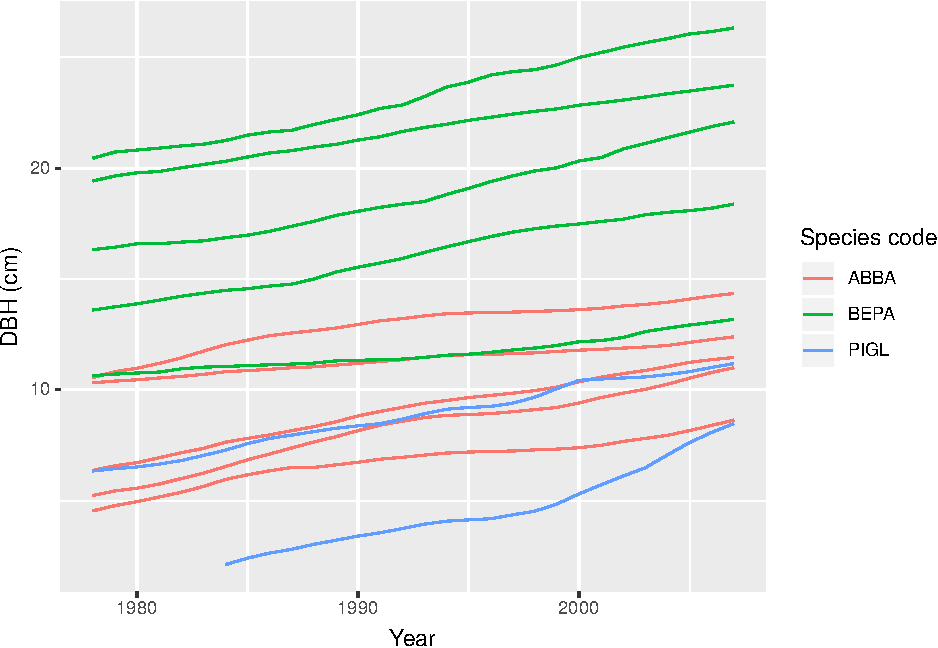
\includegraphics{bookdown_files/figure-latex/mntrees-1} 

}

\caption{Tree core derived diameter at breast height (DBH cm) by year for sampled trees in Stand 1}\label{fig:mntrees}
\end{figure}

\section{Improved Data Frames}\label{improved-data-frames}

The \texttt{dplyr} package provides two functions that offer
improvements on data frames. First, the \texttt{data\_frame} function is
a trimmed down version of the \texttt{data.frame} that is somewhat more
user friendly, and won't be discussed here. Second, the \texttt{tbl\_df}
function creates a data frame like object called a tibble\footnote{Reminds
  me of
  \href{https://en.wikipedia.org/wiki/The_Trouble_with_Tribbles}{The
  Trouble with Tribbles}}. A tibble has two advantages over a data
frame. First, when printing, it only prints the first ten rows and the
columns that fit on the page, as well as some additional information
about the table's dimension, data type of variables, and non-printed
columns. Second, recall that subsetting a data frame can sometimes
return a vector rather than a data frame (if only one row or column is
the result of the subset). A tibble does not have this behavior. Here is
an example using the \texttt{mn.trees} data frame.

\begin{Shaded}
\begin{Highlighting}[]
\OperatorTok{>}\StringTok{ }\KeywordTok{is.data.frame}\NormalTok{(mn.trees[, }\DecValTok{1}\NormalTok{])}
\end{Highlighting}
\end{Shaded}

\begin{verbatim}
[1] FALSE
\end{verbatim}

\begin{Shaded}
\begin{Highlighting}[]
\OperatorTok{>}\StringTok{ }\KeywordTok{is.vector}\NormalTok{(mn.trees[, }\DecValTok{1}\NormalTok{])}
\end{Highlighting}
\end{Shaded}

\begin{verbatim}
[1] TRUE
\end{verbatim}

\begin{Shaded}
\begin{Highlighting}[]
\OperatorTok{>}\StringTok{ }\NormalTok{mn.trees.tbl <-}\StringTok{ }\KeywordTok{tbl_df}\NormalTok{(mn.trees)}
\OperatorTok{>}\StringTok{ }\KeywordTok{is.tbl}\NormalTok{(mn.trees.tbl[, }\DecValTok{1}\NormalTok{])}
\end{Highlighting}
\end{Shaded}

\begin{verbatim}
[1] TRUE
\end{verbatim}

\begin{Shaded}
\begin{Highlighting}[]
\OperatorTok{>}\StringTok{ }\KeywordTok{is.data.frame}\NormalTok{(mn.trees.tbl[, }\DecValTok{1}\NormalTok{])}
\end{Highlighting}
\end{Shaded}

\begin{verbatim}
[1] TRUE
\end{verbatim}

\begin{Shaded}
\begin{Highlighting}[]
\OperatorTok{>}\StringTok{ }\NormalTok{mn.trees.tbl[, }\DecValTok{1}\NormalTok{]}
\end{Highlighting}
\end{Shaded}

\begin{verbatim}
# A tibble: 15,301 x 1
   StandID
     <int>
 1       1
 2       1
 3       1
 4       1
 5       1
 6       1
 7       1
 8       1
 9       1
10       1
# ... with 15,291 more rows
\end{verbatim}

Note, above that once the data frame is reduced to one dimension by
subsetting to one column, it is no longer a data frame it has been
\emph{simplified} to a vector. This might not seem like a big deal;
however, it can be very frustrating and potentially break your code when
you expect an object to behave like a data frame and it doesn't because
it's now a vector. Alternatively, once we convert \texttt{mn.trees} to a
tibble via the \texttt{tbl\_df} function the object remains a data frame
even when subset down to one dimension (there is no automatic
simplification). Converting data frames using \texttt{tbl\_df()} is not
required for using \texttt{dplyr} but is convenient. Also, it is
important to note that \texttt{tbl\_df} is simply a wrapper around a
data frame that provides some additional behaviors. The newly formed
\texttt{tbl\_df} object will still behave like a data frame (because it
technically still is a data frame) but will have some added niceties
(some of which are illustrated below).

\section{Filtering Data By Row}\label{filtering-data-by-row}

Filtering creates row subsets of data that satisfy a logical statement.
Considering the \texttt{mn.trees} data, the \texttt{filter} function can
be used to examine a particular set of stands, plots, trees, measurement
years, species, etc. The first argument in the \texttt{filter} function
is the data frame or tibble from which you want to select the rows based
on the logical statement given in the second argument. As you work
through this chapter, you'll notice the data are specified in the first
argument of all \texttt{dplyr}'s functions. Below are several
illustrative applications of the \texttt{filter} function.

\begin{Shaded}
\begin{Highlighting}[]
\OperatorTok{>}\StringTok{ }\KeywordTok{filter}\NormalTok{(mn.trees.tbl, StandID }\OperatorTok{==}\StringTok{ }\DecValTok{5}\NormalTok{)}
\end{Highlighting}
\end{Shaded}

\begin{verbatim}
# A tibble: 450 x 10
   StandID PlotID TreeID Species  Year   Age   DBH
     <int>  <int>  <int> <fct>   <int> <int> <dbl>
 1       5     13     57 ABBA     1978     2  1.71
 2       5     13     57 ABBA     1979     3  2.12
 3       5     13     57 ABBA     1980     4  2.53
 4       5     13     57 ABBA     1981     5  2.97
 5       5     13     57 ABBA     1982     6  3.48
 6       5     13     57 ABBA     1983     7  3.98
 7       5     13     57 ABBA     1984     8  4.33
 8       5     13     57 ABBA     1985     9  4.70
 9       5     13     57 ABBA     1986    10  5.07
10       5     13     57 ABBA     1987    11  5.39
# ... with 440 more rows, and 3 more variables:
#   rad.inc <dbl>, BA.inc <dbl>, UTreeID <int>
\end{verbatim}

\begin{Shaded}
\begin{Highlighting}[]
\OperatorTok{>}\StringTok{ }\KeywordTok{filter}\NormalTok{(mn.trees.tbl, Species }\OperatorTok\StringTok{ }\KeywordTok{c}\NormalTok{(}\StringTok{"ABBA"}\NormalTok{, }\StringTok{"PIST"}\NormalTok{))}
\end{Highlighting}
\end{Shaded}

\begin{verbatim}
# A tibble: 2,876 x 10
   StandID PlotID TreeID Species  Year   Age   DBH
     <int>  <int>  <int> <fct>   <int> <int> <dbl>
 1       1      1      1 ABBA     1978    19  5.23
 2       1      1      1 ABBA     1979    20  5.44
 3       1      1      1 ABBA     1980    21  5.56
 4       1      1      1 ABBA     1981    22  5.75
 5       1      1      1 ABBA     1982    23  5.99
 6       1      1      1 ABBA     1983    24  6.24
 7       1      1      1 ABBA     1984    25  6.53
 8       1      1      1 ABBA     1985    26  6.84
 9       1      1      1 ABBA     1986    27  7.10
10       1      1      1 ABBA     1987    28  7.38
# ... with 2,866 more rows, and 3 more variables:
#   rad.inc <dbl>, BA.inc <dbl>, UTreeID <int>
\end{verbatim}

\begin{Shaded}
\begin{Highlighting}[]
\OperatorTok{>}\StringTok{ }\KeywordTok{filter}\NormalTok{(mn.trees.tbl, DBH }\OperatorTok{>}\StringTok{ }\DecValTok{12} \OperatorTok{&}\StringTok{ }\NormalTok{Year }\OperatorTok{==}\StringTok{ }\DecValTok{1980}\NormalTok{)}
\end{Highlighting}
\end{Shaded}

\begin{verbatim}
# A tibble: 228 x 10
   StandID PlotID TreeID Species  Year   Age   DBH
     <int>  <int>  <int> <fct>   <int> <int> <dbl>
 1       1      1      4 BEPA     1980    74  16.6
 2       1      2      8 BEPA     1980    92  19.8
 3       1      2      9 BEPA     1980    75  13.9
 4       1      2     10 BEPA     1980    98  20.8
 5       2      4     14 BEPA     1980    98  19.5
 6       2      4     15 BEPA     1980   124  21.3
 7       2      4     16 BEPA     1980   116  18.4
 8       2      4     17 PIGL     1980    34  12.6
 9       2      5     18 PIGL     1980    34  12.4
10       2      5     19 PIRE     1980   242  58.4
# ... with 218 more rows, and 3 more variables:
#   rad.inc <dbl>, BA.inc <dbl>, UTreeID <int>
\end{verbatim}

\begin{Shaded}
\begin{Highlighting}[]
\OperatorTok{>}\StringTok{ }\KeywordTok{filter}\NormalTok{(mn.trees.tbl, Species }\OperatorTok\StringTok{ }\KeywordTok{c}\NormalTok{(}\StringTok{"ABBA"}\NormalTok{, }\StringTok{"PIST"}\NormalTok{) }\OperatorTok{&}\StringTok{ }\NormalTok{Year }\OperatorTok{==}\StringTok{ }
\OperatorTok{+}\StringTok{   }\DecValTok{1985}\NormalTok{)}
\end{Highlighting}
\end{Shaded}

\begin{verbatim}
# A tibble: 87 x 10
   StandID PlotID TreeID Species  Year   Age   DBH
     <int>  <int>  <int> <fct>   <int> <int> <dbl>
 1       1      1      1 ABBA     1985    26  6.84
 2       1      1      2 ABBA     1985    41  7.81
 3       1      2      6 ABBA     1985    19  6.16
 4       1      2      7 ABBA     1985    16 10.9 
 5       1      3     11 ABBA     1985    40 12.2 
 6       2      5     21 PIST     1985   149 35.9 
 7       2      6     22 ABBA     1985    33 12.3 
 8       3      7     28 PIST     1985    49 10.5 
 9       3      7     29 PIST     1985    48 17.7 
10       3      7     30 PIST     1985    52 22.4 
# ... with 77 more rows, and 3 more variables:
#   rad.inc <dbl>, BA.inc <dbl>, UTreeID <int>
\end{verbatim}

Notice the full results are not printed. For example, when we asked for
the data for stand 5, only the first ten rows were printed. This is an
effect of using the \texttt{tbl\_df} function. Of course if we wanted to
analyze the results (as we will below) the full set of data would be
available.

\section{Selecting Variables by
Column}\label{selecting-variables-by-column}

Another common task is to restrict attention to some subset of variables
in the data set. This is accomplished using the \texttt{select}
function. Like \texttt{filter}, the data frame or tibble is the first
argument in the \texttt{select} function, followed by additional
arguments identifying variables you want to include or exclude. Consider
the examples below.

\begin{Shaded}
\begin{Highlighting}[]
\OperatorTok{>}\StringTok{ }\KeywordTok{select}\NormalTok{(mn.trees.tbl, Year, DBH)}
\end{Highlighting}
\end{Shaded}

\begin{verbatim}
# A tibble: 15,301 x 2
    Year   DBH
   <int> <dbl>
 1  1978  5.23
 2  1979  5.44
 3  1980  5.56
 4  1981  5.75
 5  1982  5.99
 6  1983  6.24
 7  1984  6.53
 8  1985  6.84
 9  1986  7.10
10  1987  7.38
# ... with 15,291 more rows
\end{verbatim}

\begin{Shaded}
\begin{Highlighting}[]
\OperatorTok{>}\StringTok{ }\KeywordTok{select}\NormalTok{(mn.trees.tbl, }\DecValTok{2}\OperatorTok{:}\DecValTok{4}\NormalTok{)}
\end{Highlighting}
\end{Shaded}

\begin{verbatim}
# A tibble: 15,301 x 3
   PlotID TreeID Species
    <int>  <int> <fct>  
 1      1      1 ABBA   
 2      1      1 ABBA   
 3      1      1 ABBA   
 4      1      1 ABBA   
 5      1      1 ABBA   
 6      1      1 ABBA   
 7      1      1 ABBA   
 8      1      1 ABBA   
 9      1      1 ABBA   
10      1      1 ABBA   
# ... with 15,291 more rows
\end{verbatim}

\begin{Shaded}
\begin{Highlighting}[]
\OperatorTok{>}\StringTok{ }\KeywordTok{select}\NormalTok{(mn.trees.tbl, }\OperatorTok{-}\KeywordTok{c}\NormalTok{(}\DecValTok{2}\NormalTok{, }\DecValTok{3}\NormalTok{, }\DecValTok{4}\NormalTok{))}
\end{Highlighting}
\end{Shaded}

\begin{verbatim}
# A tibble: 15,301 x 7
   StandID  Year   Age   DBH rad.inc BA.inc UTreeID
     <int> <int> <int> <dbl>   <dbl>  <dbl>   <int>
 1       1  1978    19  5.23   0.92    1.48       1
 2       1  1979    20  5.44   1.03    1.73       1
 3       1  1980    21  5.56   0.61    1.05       1
 4       1  1981    22  5.75   0.935   1.66       1
 5       1  1982    23  5.99   1.25    2.30       1
 6       1  1983    24  6.24   1.20    2.31       1
 7       1  1984    25  6.53   1.50    3.00       1
 8       1  1985    26  6.84   1.54    3.25       1
 9       1  1986    27  7.10   1.28    2.81       1
10       1  1987    28  7.38   1.38    3.14       1
# ... with 15,291 more rows
\end{verbatim}

\begin{Shaded}
\begin{Highlighting}[]
\OperatorTok{>}\StringTok{ }\KeywordTok{select}\NormalTok{(mn.trees.tbl, }\KeywordTok{ends_with}\NormalTok{(}\StringTok{"ID"}\NormalTok{))}
\end{Highlighting}
\end{Shaded}

\begin{verbatim}
# A tibble: 15,301 x 4
   StandID PlotID TreeID UTreeID
     <int>  <int>  <int>   <int>
 1       1      1      1       1
 2       1      1      1       1
 3       1      1      1       1
 4       1      1      1       1
 5       1      1      1       1
 6       1      1      1       1
 7       1      1      1       1
 8       1      1      1       1
 9       1      1      1       1
10       1      1      1       1
# ... with 15,291 more rows
\end{verbatim}

Notice a few things. Variables can be selected by name or column number.
As usual a negative sign tells R to leave something out. Also, there are
special \emph{helper} functions such as \texttt{ends\_with} that provide
ways to match part of a variable's name. Other very handy helper
functions you should investigate are \texttt{begins\_with},
\texttt{contains}, \texttt{matches}, \texttt{num\_range},
\texttt{one\_of}, and \texttt{everything}.

\section{Pipes}\label{pipes}

Consider selecting the \texttt{Age} and \texttt{rad.inc} for the two
aspen species POTR or POGR (\emph{Populus tremuloides} and \emph{Populus
grandifolia}). One possibility is to nest a \texttt{filter} call within
\texttt{select}.

\begin{Shaded}
\begin{Highlighting}[]
\OperatorTok{>}\StringTok{ }\KeywordTok{select}\NormalTok{(}\KeywordTok{filter}\NormalTok{(mn.trees.tbl, Species }\OperatorTok\StringTok{ }\KeywordTok{c}\NormalTok{(}\StringTok{"POTR"}\NormalTok{, }\StringTok{"POGR"}\NormalTok{)), }
\OperatorTok{+}\StringTok{   }\NormalTok{Age, rad.inc)}
\end{Highlighting}
\end{Shaded}

\begin{verbatim}
# A tibble: 719 x 2
     Age rad.inc
   <int>   <dbl>
 1    55   0.935
 2    56   0.7  
 3    57   0.25 
 4    58   0.595
 5    59   1.28 
 6    60   1.34 
 7    61   1.14 
 8    62   1.20 
 9    63   1.09 
10    64   0.975
# ... with 709 more rows
\end{verbatim}

Even a two-step process like this becomes hard to follow in this nested
form, and often we will want to perform more than two operations. There
is a nice feature in \texttt{dplyr} that allows us to ``feed'' results
of one function into the first argument of a subsequent function.
Another way of saying this is that we are ``piping'' the results into
another function. The \texttt{\%\textgreater{}\%} operator does the
piping.

\begin{Shaded}
\begin{Highlighting}[]
\OperatorTok{>}\StringTok{ }\NormalTok{mn.trees.tbl }\OperatorTok\StringTok{ }
\OperatorTok{+}\StringTok{   }\KeywordTok{filter}\NormalTok{(Species }\OperatorTok\StringTok{ }\KeywordTok{c}\NormalTok{(}\StringTok{"POTR"}\NormalTok{, }\StringTok{"POGR"}\NormalTok{)) }\OperatorTok\StringTok{ }
\OperatorTok{+}\StringTok{   }\KeywordTok{select}\NormalTok{(Age, rad.inc)}
\end{Highlighting}
\end{Shaded}

\begin{verbatim}
# A tibble: 719 x 2
     Age rad.inc
   <int>   <dbl>
 1    55   0.935
 2    56   0.7  
 3    57   0.25 
 4    58   0.595
 5    59   1.28 
 6    60   1.34 
 7    61   1.14 
 8    62   1.20 
 9    63   1.09 
10    64   0.975
# ... with 709 more rows
\end{verbatim}

It can help to think of \texttt{\%\textgreater{}\%} as representing the
word ``then.'' The above can be read as, ``Start with the data frame
\texttt{mn.trees.tbl}, \emph{then} filter it to select data from the
species POTR and POGR, \emph{then} select the variables age and radial
growth increment from these data.''

The pipe operator \texttt{\%\textgreater{}\%} is not restricted to
functions in \texttt{dplyr}. In fact the pipe operator itself was
introduced in another package called \texttt{magrittr}, but is included
in \texttt{dplyr} as a convenience.

\section{Arranging Data by Row}\label{arranging-data-by-row}

By default the \texttt{mn.trees} data are arranged in ascending order by
\texttt{StandID}, then \texttt{PlotID}, then \texttt{TreeID}, then
\texttt{Year}.

\begin{Shaded}
\begin{Highlighting}[]
\OperatorTok{>}\StringTok{ }\KeywordTok{head}\NormalTok{(mn.trees.tbl, }\DecValTok{5}\NormalTok{)}
\end{Highlighting}
\end{Shaded}

\begin{verbatim}
# A tibble: 5 x 10
  StandID PlotID TreeID Species  Year   Age   DBH
    <int>  <int>  <int> <fct>   <int> <int> <dbl>
1       1      1      1 ABBA     1978    19  5.23
2       1      1      1 ABBA     1979    20  5.44
3       1      1      1 ABBA     1980    21  5.56
4       1      1      1 ABBA     1981    22  5.75
5       1      1      1 ABBA     1982    23  5.99
# ... with 3 more variables: rad.inc <dbl>,
#   BA.inc <dbl>, UTreeID <int>
\end{verbatim}

\begin{Shaded}
\begin{Highlighting}[]
\OperatorTok{>}\StringTok{ }\KeywordTok{tail}\NormalTok{(mn.trees.tbl, }\DecValTok{5}\NormalTok{)}
\end{Highlighting}
\end{Shaded}

\begin{verbatim}
# A tibble: 5 x 10
  StandID PlotID TreeID Species  Year   Age   DBH
    <int>  <int>  <int> <fct>   <int> <int> <dbl>
1      35    105    521 POTR     2003    32  17.5
2      35    105    521 POTR     2004    33  17.6
3      35    105    521 POTR     2005    34  17.9
4      35    105    521 POTR     2006    35  18.1
5      35    105    521 POTR     2007    36  18.2
# ... with 3 more variables: rad.inc <dbl>,
#   BA.inc <dbl>, UTreeID <int>
\end{verbatim}

This is convenient ordering for these data. But what if we wanted to
change the order to be by \texttt{Species} then \texttt{Year}? The
\texttt{arrange} function makes this easy. The following examples
illustrate \texttt{arrange} but also use pipes to simplify code and
\texttt{select} to focus attention on the columns of interest.

Let's start with arranging in ascending order \texttt{BA.inc} for tree 1
in plot 1 in stand 1.

\begin{Shaded}
\begin{Highlighting}[]
\OperatorTok{>}\StringTok{ }\NormalTok{mn.trees.tbl }\OperatorTok\StringTok{ }
\OperatorTok{+}\StringTok{   }\KeywordTok{filter}\NormalTok{(StandID }\OperatorTok{==}\StringTok{ }\DecValTok{1} \OperatorTok{&}\StringTok{ }\NormalTok{PlotID }\OperatorTok{==}\StringTok{ }\DecValTok{1} \OperatorTok{&}\StringTok{ }\NormalTok{TreeID }\OperatorTok{==}\StringTok{ }\DecValTok{1}\NormalTok{) }\OperatorTok\StringTok{ }
\OperatorTok{+}\StringTok{   }\KeywordTok{select}\NormalTok{(StandID, PlotID, TreeID, BA.inc) }\OperatorTok\StringTok{ }
\OperatorTok{+}\StringTok{   }\KeywordTok{arrange}\NormalTok{(BA.inc) }
\end{Highlighting}
\end{Shaded}

\begin{verbatim}
# A tibble: 30 x 4
   StandID PlotID TreeID BA.inc
     <int>  <int>  <int>  <dbl>
 1       1      1      1  0.501
 2       1      1      1  0.615
 3       1      1      1  1.05 
 4       1      1      1  1.18 
 5       1      1      1  1.35 
 6       1      1      1  1.38 
 7       1      1      1  1.42 
 8       1      1      1  1.48 
 9       1      1      1  1.66 
10       1      1      1  1.73 
# ... with 20 more rows
\end{verbatim}

Possibly we want these data to be in decreasing (descending) order.
Here, \texttt{desc()} is one of many \texttt{dplyr} helper functions.

\begin{Shaded}
\begin{Highlighting}[]
\OperatorTok{>}\StringTok{ }\NormalTok{mn.trees.tbl }\OperatorTok\StringTok{ }
\OperatorTok{+}\StringTok{   }\KeywordTok{filter}\NormalTok{(StandID }\OperatorTok{==}\StringTok{ }\DecValTok{1} \OperatorTok{&}\StringTok{ }\NormalTok{PlotID }\OperatorTok{==}\StringTok{ }\DecValTok{1} \OperatorTok{&}\StringTok{ }\NormalTok{TreeID }\OperatorTok{==}\StringTok{ }\DecValTok{1}\NormalTok{) }\OperatorTok\StringTok{ }
\OperatorTok{+}\StringTok{   }\KeywordTok{select}\NormalTok{(StandID, PlotID, TreeID, BA.inc) }\OperatorTok\StringTok{ }
\OperatorTok{+}\StringTok{   }\KeywordTok{arrange}\NormalTok{(}\KeywordTok{desc}\NormalTok{(BA.inc))}
\end{Highlighting}
\end{Shaded}

\begin{verbatim}
# A tibble: 30 x 4
   StandID PlotID TreeID BA.inc
     <int>  <int>  <int>  <dbl>
 1       1      1      1   4.45
 2       1      1      1   4.33
 3       1      1      1   3.67
 4       1      1      1   3.65
 5       1      1      1   3.59
 6       1      1      1   3.46
 7       1      1      1   3.25
 8       1      1      1   3.23
 9       1      1      1   3.16
10       1      1      1   3.14
# ... with 20 more rows
\end{verbatim}

Passing multiple variables to \texttt{arrange} results in nested
ordering. The subsequent code orders first by \texttt{Species}, then
\texttt{Year} within \texttt{Species}, then \texttt{BA.inc} within
\texttt{Year} and \texttt{Species}.

\begin{Shaded}
\begin{Highlighting}[]
\OperatorTok{>}\StringTok{ }\NormalTok{mn.trees.tbl }\OperatorTok\StringTok{ }
\OperatorTok{+}\StringTok{   }\KeywordTok{select}\NormalTok{(Species, Year, BA.inc) }\OperatorTok\StringTok{ }
\OperatorTok{+}\StringTok{   }\KeywordTok{arrange}\NormalTok{(Species, Year, BA.inc) }
\end{Highlighting}
\end{Shaded}

\begin{verbatim}
# A tibble: 15,301 x 3
   Species  Year BA.inc
   <fct>   <int>  <dbl>
 1 ABBA     1978  0.253
 2 ABBA     1978  0.368
 3 ABBA     1978  0.416
 4 ABBA     1978  0.560
 5 ABBA     1978  0.620
 6 ABBA     1978  0.650
 7 ABBA     1978  0.672
 8 ABBA     1978  0.676
 9 ABBA     1978  0.699
10 ABBA     1978  0.760
# ... with 15,291 more rows
\end{verbatim}

For analyzing data in R, the order shouldn't matter. But for
presentation to human eyes, the order is important.

\section{Renaming Variables}\label{renaming-variables}

The \texttt{dplyr} package has a \texttt{rename} function that makes
renaming variables in a data frame quite easy. Below, I rename the
\texttt{rad.inc} and \texttt{BA.inc} to remind myself of their
measurement units (i.e., millimeters and centimeters squared,
respectively).

\begin{Shaded}
\begin{Highlighting}[]
\OperatorTok{>}\StringTok{ }\NormalTok{mn.trees.tbl <-}\StringTok{ }\KeywordTok{rename}\NormalTok{(mn.trees.tbl, }\DataTypeTok{rad.inc.mm =}\NormalTok{ rad.inc, }
\OperatorTok{+}\StringTok{                        }\DataTypeTok{BA.inc.cm2 =}\NormalTok{ BA.inc)}
\OperatorTok{>}\StringTok{ }\KeywordTok{head}\NormalTok{(mn.trees.tbl)}
\end{Highlighting}
\end{Shaded}

\begin{verbatim}
# A tibble: 6 x 10
  StandID PlotID TreeID Species  Year   Age   DBH
    <int>  <int>  <int> <fct>   <int> <int> <dbl>
1       1      1      1 ABBA     1978    19  5.23
2       1      1      1 ABBA     1979    20  5.44
3       1      1      1 ABBA     1980    21  5.56
4       1      1      1 ABBA     1981    22  5.75
5       1      1      1 ABBA     1982    23  5.99
6       1      1      1 ABBA     1983    24  6.24
# ... with 3 more variables: rad.inc.mm <dbl>,
#   BA.inc.cm2 <dbl>, UTreeID <int>
\end{verbatim}

\section{Creating New Variables}\label{creating-new-variables}

We routinely want to create new variables and add them to an existing
data frame. This task is done using the \texttt{mutate} function.
\texttt{mutate} adds new columns to the right side of your data frame or
tibble. This function is particularly useful because it can make a new
variable by simply referencing variables that exist in the data frame.
Let's start with a simple example. Below I create a small data frame
called \texttt{df} with two numeric columns \texttt{a} and \texttt{b}.
Next, I add a new variable \texttt{c} that is the square root of the sum
of \texttt{a} and \texttt{b}. We can of course use \texttt{mutate} to
add variables that are not a function of existing variables, e.g., see
the addition of the logical variable \texttt{d} below (this time using a
pipe).

\begin{Shaded}
\begin{Highlighting}[]
\OperatorTok{>}\StringTok{ }\NormalTok{df <-}\StringTok{ }\KeywordTok{data.frame}\NormalTok{(}\StringTok{"a"}\NormalTok{=}\DecValTok{1}\OperatorTok{:}\DecValTok{4}\NormalTok{, }\StringTok{"b"}\NormalTok{=}\KeywordTok{c}\NormalTok{(}\DecValTok{8}\NormalTok{, }\DecValTok{12}\NormalTok{, }\DecValTok{19}\NormalTok{, }\DecValTok{76}\NormalTok{))}
\OperatorTok{>}\StringTok{ }\NormalTok{df <-}\StringTok{ }\KeywordTok{mutate}\NormalTok{(df, }\DataTypeTok{c =} \KeywordTok{log}\NormalTok{(a}\OperatorTok{+}\NormalTok{b))}
\OperatorTok{>}\StringTok{ }\NormalTok{df}
\end{Highlighting}
\end{Shaded}

\begin{verbatim}
  a  b     c
1 1  8 2.197
2 2 12 2.639
3 3 19 3.091
4 4 76 4.382
\end{verbatim}

\begin{Shaded}
\begin{Highlighting}[]
\OperatorTok{>}\StringTok{ }\NormalTok{df <-}\StringTok{ }\NormalTok{df }\OperatorTok\StringTok{ }
\OperatorTok{+}\StringTok{   }\KeywordTok{mutate}\NormalTok{(}\DataTypeTok{d =} \KeywordTok{c}\NormalTok{(}\StringTok{"Jerry"}\NormalTok{,}\StringTok{"Jerry"}\NormalTok{,}\StringTok{"Bobby"}\NormalTok{,}\StringTok{"Bobby"}\NormalTok{))}
\OperatorTok{>}\StringTok{ }\NormalTok{df}
\end{Highlighting}
\end{Shaded}

\begin{verbatim}
  a  b     c     d
1 1  8 2.197 Jerry
2 2 12 2.639 Jerry
3 3 19 3.091 Bobby
4 4 76 4.382 Bobby
\end{verbatim}

Sometimes, we want to create new variables that are a function of
existing variables but not add them to the data frame. In this case we
use the \texttt{transmute} function. Here, I create a new data frame
\texttt{df.2} that comprises two new variables, \texttt{e} and
\texttt{f} where \texttt{e} is \texttt{a+c} and \texttt{f} is just a
copy of \texttt{d}.

\begin{Shaded}
\begin{Highlighting}[]
\OperatorTok{>}\StringTok{ }\NormalTok{df.}\DecValTok{2}\NormalTok{ <-}\StringTok{ }\NormalTok{df }\OperatorTok\StringTok{ }\KeywordTok{transmute}\NormalTok{(}\DataTypeTok{e =}\NormalTok{ a }\OperatorTok{+}\StringTok{ }\NormalTok{c, }\DataTypeTok{f =}\NormalTok{ d)}
\OperatorTok{>}\StringTok{ }\NormalTok{df.}\DecValTok{2}
\end{Highlighting}
\end{Shaded}

\begin{verbatim}
      e     f
1 3.197 Jerry
2 4.639 Jerry
3 6.091 Bobby
4 8.382 Bobby
\end{verbatim}

\section{Data Summaries and Grouping}\label{data-summaries-and-grouping}

The \texttt{summarize} function computes summary statistics or user
provided functions for one or more variables in a data frame. Below, the
\texttt{summarize} function is used to calculate the mean and sum of
variable \texttt{a} in the data frame created in the previous section.

\begin{Shaded}
\begin{Highlighting}[]
\OperatorTok{>}\StringTok{ }\KeywordTok{summarize}\NormalTok{(df, }\DataTypeTok{a.mean =} \KeywordTok{mean}\NormalTok{(a), }\DataTypeTok{a.sum =} \KeywordTok{sum}\NormalTok{(a))}
\end{Highlighting}
\end{Shaded}

\begin{verbatim}
  a.mean a.sum
1    2.5    10
\end{verbatim}

\begin{Shaded}
\begin{Highlighting}[]
\OperatorTok{>}\StringTok{ }\NormalTok{##or}
\ErrorTok{>}\StringTok{ }\NormalTok{df }\OperatorTok\StringTok{ }
\OperatorTok{+}\StringTok{   }\KeywordTok{summarize}\NormalTok{(}\DataTypeTok{a.mean =} \KeywordTok{mean}\NormalTok{(a), }\DataTypeTok{a.sum =} \KeywordTok{sum}\NormalTok{(a))}
\end{Highlighting}
\end{Shaded}

\begin{verbatim}
  a.mean a.sum
1    2.5    10
\end{verbatim}

By itself, \texttt{summarize} is of limited use. Often we want row
summaries for specific components of the data. For example, say we want
to sum variable \texttt{a} for each category of variable \texttt{d}. One
option is to subset and summarize for each category in \texttt{b}:

\begin{Shaded}
\begin{Highlighting}[]
\OperatorTok{>}\StringTok{ }\NormalTok{df }\OperatorTok\StringTok{ }
\OperatorTok{+}\StringTok{   }\KeywordTok{filter}\NormalTok{(d }\OperatorTok{==}\StringTok{ "Jerry"}\NormalTok{) }\OperatorTok\StringTok{ }
\OperatorTok{+}\StringTok{   }\KeywordTok{summarize}\NormalTok{(}\DataTypeTok{a.sum =} \KeywordTok{sum}\NormalTok{(a))}
\end{Highlighting}
\end{Shaded}

\begin{verbatim}
  a.sum
1     3
\end{verbatim}

\begin{Shaded}
\begin{Highlighting}[]
\OperatorTok{>}\StringTok{ }\NormalTok{df }\OperatorTok\StringTok{ }
\OperatorTok{+}\StringTok{   }\KeywordTok{filter}\NormalTok{(d }\OperatorTok{==}\StringTok{ "Bobby"}\NormalTok{) }\OperatorTok\StringTok{ }
\OperatorTok{+}\StringTok{   }\KeywordTok{summarize}\NormalTok{(}\DataTypeTok{a.sum =} \KeywordTok{sum}\NormalTok{(a))}
\end{Highlighting}
\end{Shaded}

\begin{verbatim}
  a.sum
1     7
\end{verbatim}

This is a very tedious approach if the number of subsets is large. Also,
we might want the result as a single data frame, which means we would
need to then combine the summaries of all the subsets in a subsequent
step.

The \texttt{group\_by} function used in combination with
\texttt{summarize} simplifies this task and makes the output more
useful. The \texttt{summarize} function is applied to each category in
the \emph{grouping} variable specified in \texttt{group\_by}, as
illustrated in the code below.

\begin{Shaded}
\begin{Highlighting}[]
\OperatorTok{>}\StringTok{ }\NormalTok{df }\OperatorTok\StringTok{ }
\OperatorTok{+}\StringTok{   }\KeywordTok{group_by}\NormalTok{(d) }\OperatorTok\StringTok{ }
\OperatorTok{+}\StringTok{   }\KeywordTok{summarize}\NormalTok{(}\DataTypeTok{a.sum =} \KeywordTok{sum}\NormalTok{(a)) }
\end{Highlighting}
\end{Shaded}

\begin{verbatim}
# A tibble: 2 x 2
  d     a.sum
  <chr> <int>
1 Bobby     7
2 Jerry     3
\end{verbatim}

We can specify multiple variables with \texttt{group\_by} to define the
categories to summarize. Let's return to the \texttt{mn.trees} data set
and find the sum of annual radial growth increment by species within
each stand.

\begin{Shaded}
\begin{Highlighting}[]
\OperatorTok{>}\StringTok{ }\NormalTok{stand.spp <-}\StringTok{ }\NormalTok{mn.trees.tbl }\OperatorTok\StringTok{ }
\OperatorTok{+}\StringTok{   }\KeywordTok{group_by}\NormalTok{(StandID, Species) }\OperatorTok\StringTok{ }
\OperatorTok{+}\StringTok{   }\KeywordTok{summarize}\NormalTok{(}\DataTypeTok{rad.inc.total =} \KeywordTok{sum}\NormalTok{(rad.inc.mm), }
\OperatorTok{+}\StringTok{             }\DataTypeTok{BA.inc.total =} \KeywordTok{sum}\NormalTok{(BA.inc.cm2))}
\OperatorTok{>}\StringTok{ }\NormalTok{stand.spp}
\end{Highlighting}
\end{Shaded}

\begin{verbatim}
# A tibble: 115 x 4
# Groups:   StandID [?]
   StandID Species rad.inc.total BA.inc.total
     <int> <fct>           <dbl>        <dbl>
 1       1 ABBA            109.         309. 
 2       1 BEPA            122.         733. 
 3       1 PIGL             58.0        121. 
 4       2 ABBA             88.8        262. 
 5       2 BEPA            101.         488. 
 6       2 PIGL             86.3        431. 
 7       2 PIRE             35.7        510. 
 8       2 PIST             60.3        749. 
 9       3 ABBA             57.6        135. 
10       3 PIGL             21.1         94.8
# ... with 105 more rows
\end{verbatim}

There are several things to notice here. Our code specifies both
\texttt{StandID} and \texttt{Species} variables in the
\texttt{group\_by} function, which causes \texttt{summarize} arguments
to be applied to each stand and species combination. For example,
looking at the output, we can see that stand 1 contains three species
\texttt{ABBA} (\emph{Abies balsamea}), \texttt{BEPA} (\emph{Betula
papyrifera}), and \texttt{PIGL} (\emph{Picea glauca}). Also, for each of
these species, the sum of radial growth increments, i.e.,
\texttt{rad.inc.total}, is 108.735, 121.515, and 58.045, and the sum of
basal area growth increments, i.e., \texttt{BA.inc.total}, is
approximately 308.98, 732.58, and 121.26. The two commented lines above
the resulting tibble tell us there are 115 such stand and species
combinations, i.e., \texttt{\#\ A\ tibble:\ 115\ x\ 4}, and the tibble
is grouped by \texttt{StandID}, i.e.,
\texttt{\#\ Groups:\ StandID\ {[}?{]}}. This last bit of information is
important. Recall a tibble is a data frame with some additional
functionality. Not only does the resulting tibble hold the
\texttt{summarize} output, it also retains all levels of grouping to the
left of the last grouping variable specified in \texttt{group\_by}. In
this case we grouped by \texttt{StandID} and \texttt{Species} prior to
calling \texttt{summarize}, so the resulting tibble is grouped by
\texttt{StandID}. If we fed the resulting tibble back into
\texttt{summarize}, aggregation would occur for each stand. Depending on
the analysis, this retention of grouping can be handy or annoying. If
necessary, use \texttt{ungroup} to remove the grouping from a tibble,
e.g., \texttt{stand.spp\ \%\textgreater{}\%\ ungroup()}.

\section{Counts}\label{counts}

In many circumstances it is useful to know how many rows are being
summarized. Continuing the previous example, say we want to know how
many increment measurements comprise a given \texttt{StandID} and
\texttt{Species} combination and, hence, went into the
\texttt{rad.inc.total} and \texttt{BA.inc.total} summaries. The
\texttt{n} function returns the count of rows per group (or number of
rows in an ungrouped tibble). Below, I add a new variable called
\texttt{n.inc} to the our previous \texttt{stand.spp}.

\begin{Shaded}
\begin{Highlighting}[]
\OperatorTok{>}\StringTok{ }\NormalTok{stand.spp <-}\StringTok{ }\NormalTok{mn.trees.tbl }\OperatorTok
\OperatorTok{+}\StringTok{   }\KeywordTok{group_by}\NormalTok{(StandID, Species) }\OperatorTok\StringTok{ }
\OperatorTok{+}\StringTok{   }\KeywordTok{summarize}\NormalTok{(}\DataTypeTok{rad.inc.total =} \KeywordTok{sum}\NormalTok{(rad.inc.mm), }
\OperatorTok{+}\StringTok{             }\DataTypeTok{BA.inc.total =} \KeywordTok{sum}\NormalTok{(BA.inc.cm2),}
\OperatorTok{+}\StringTok{             }\DataTypeTok{n.inc =} \KeywordTok{n}\NormalTok{())}
\OperatorTok{>}\StringTok{ }\NormalTok{stand.spp}
\end{Highlighting}
\end{Shaded}

\begin{verbatim}
# A tibble: 115 x 5
# Groups:   StandID [?]
   StandID Species rad.inc.total BA.inc.total n.inc
     <int> <fct>           <dbl>        <dbl> <int>
 1       1 ABBA            109.         309.    150
 2       1 BEPA            122.         733.    150
 3       1 PIGL             58.0        121.     54
 4       2 ABBA             88.8        262.     45
 5       2 BEPA            101.         488.    180
 6       2 PIGL             86.3        431.     90
 7       2 PIRE             35.7        510.     60
 8       2 PIST             60.3        749.     30
 9       3 ABBA             57.6        135.     30
10       3 PIGL             21.1         94.8    60
# ... with 105 more rows
\end{verbatim}

This is helpful. We now know how many individual increment measurements
were used to compute the summaries. However, it is not clear how many
trees were actually cored to generate these measurements. We can get at
the count of unique trees in each group by using the
\texttt{n\_distinct} helper function.

\begin{Shaded}
\begin{Highlighting}[]
\OperatorTok{>}\StringTok{ }\NormalTok{stand.spp <-}\StringTok{ }\NormalTok{mn.trees.tbl }\OperatorTok\StringTok{ }\KeywordTok{group_by}\NormalTok{(StandID, Species) }\OperatorTok\StringTok{ }
\OperatorTok{+}\StringTok{     }\KeywordTok{summarize}\NormalTok{(}\DataTypeTok{rad.inc.total =} \KeywordTok{sum}\NormalTok{(rad.inc.mm), }
\OperatorTok{+}\StringTok{               }\DataTypeTok{BA.inc.total =} \KeywordTok{sum}\NormalTok{(BA.inc.cm2),}
\OperatorTok{+}\StringTok{               }\DataTypeTok{n.inc =} \KeywordTok{n}\NormalTok{(),}
\OperatorTok{+}\StringTok{               }\DataTypeTok{n.trees =} \KeywordTok{n_distinct}\NormalTok{(PlotID, TreeID))}
\OperatorTok{>}\StringTok{ }\NormalTok{stand.spp}
\end{Highlighting}
\end{Shaded}

\begin{verbatim}
# A tibble: 115 x 6
# Groups:   StandID [?]
   StandID Species rad.inc.total BA.inc.total n.inc
     <int> <fct>           <dbl>        <dbl> <int>
 1       1 ABBA            109.         309.    150
 2       1 BEPA            122.         733.    150
 3       1 PIGL             58.0        121.     54
 4       2 ABBA             88.8        262.     45
 5       2 BEPA            101.         488.    180
 6       2 PIGL             86.3        431.     90
 7       2 PIRE             35.7        510.     60
 8       2 PIST             60.3        749.     30
 9       3 ABBA             57.6        135.     30
10       3 PIGL             21.1         94.8    60
# ... with 105 more rows, and 1 more variable:
#   n.trees <int>
\end{verbatim}

Recall, \texttt{StandID}, \texttt{PlotID}, and \texttt{TreeID}
identifies the set of increment measurements for a specific tree.
Therefore, if we group using \texttt{StandID}, then
\texttt{n\_distinct(PlotID,\ TreeID)} returns the unique tree count
within each stand. Above, we also group by \texttt{Species} so the
unique tree count within the stand is also partitioned by species. Now,
we can see the new variable \texttt{n.trees} is the number of trees by
species over which \texttt{n.inc} increment measurements were collected.

\bibliography{text.bib}

\backmatter
\printindex

\end{document}
